% This file was converted to LaTeX by Writer2LaTeX ver. 1.4
% see http://writer2latex.sourceforge.net for more info
\documentclass{article}
\usepackage{amsmath,amssymb,amsfonts}
\usepackage{fontspec}
\usepackage{xunicode}
\usepackage{xltxtra}
\usepackage{polyglossia}
\setdefaultlanguage{spanish}
\usepackage{multicol}
\usepackage{array}
\usepackage{supertabular}
\usepackage{hhline}
\usepackage{graphicx}
\makeatletter
\newcommand\arraybslash{\let\\\@arraycr}
\makeatother
\setlength\tabcolsep{1mm}
\renewcommand\arraystretch{1.3}
\newcounter{Figura}
\renewcommand\theFigura{\arabic{Figura}}
\title{}
\begin{document}
\begin{flushleft}
\tablefirsthead{}
\tablehead{}
\tabletail{}
\tablelasttail{}
\begin{supertabular}{m{7.7320004cm}m{0.091000006cm}|m{2.421cm}|m{0.089cm}m{0.694cm}m{0.693cm}m{0.693cm}m{0.693cm}m{0.693cm}m{0.691cm}m{0.693cm}m{0.703cm}}
\hhline{~~-~~~~~~~~~}
Componente:

\begin{center}
\includegraphics{texto-img/texto-img001.jpg}
\end{center}
\begin{center}
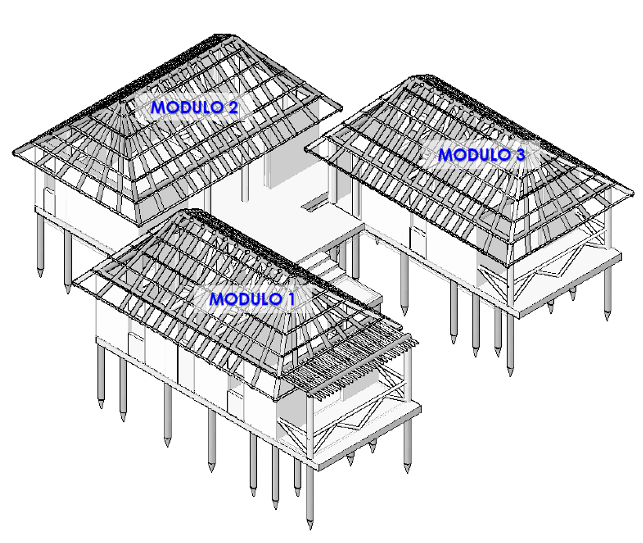
\includegraphics{texto-img/texto-img002.png}
\end{center}
\begin{center}
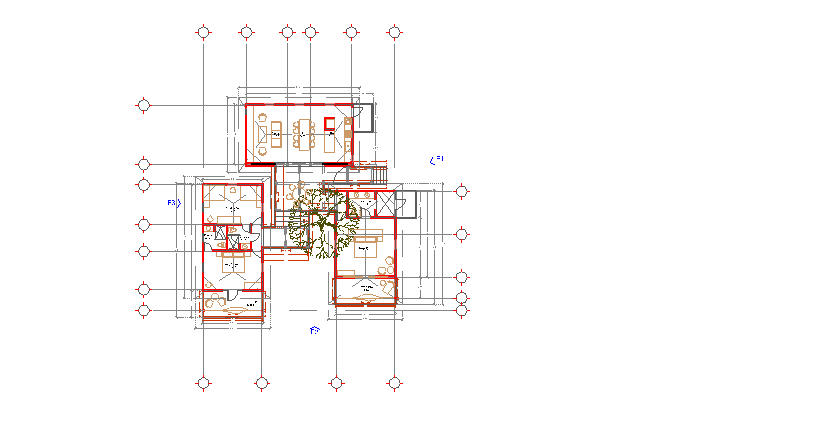
\includegraphics{texto-img/texto-img003.png}
\end{center}
\begin{center}
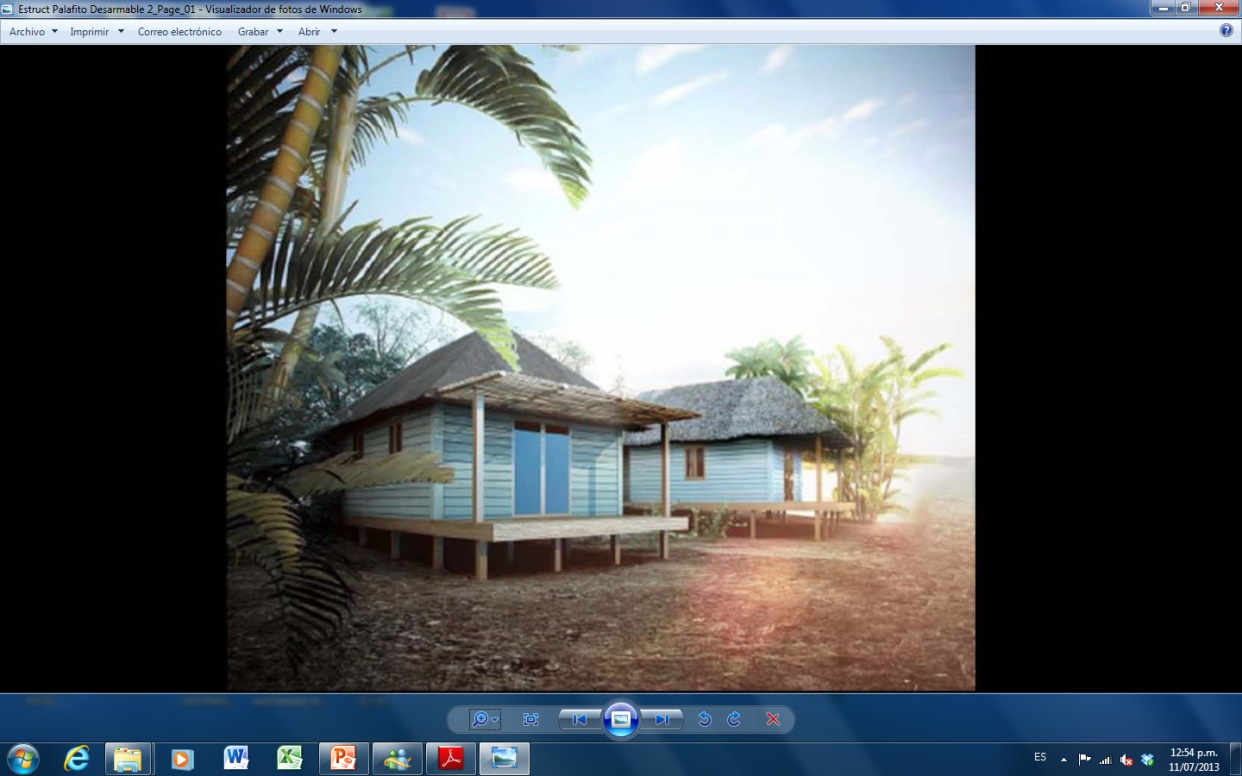
\includegraphics{texto-img/texto-img004.jpg}
\end{center}
\begin{center}
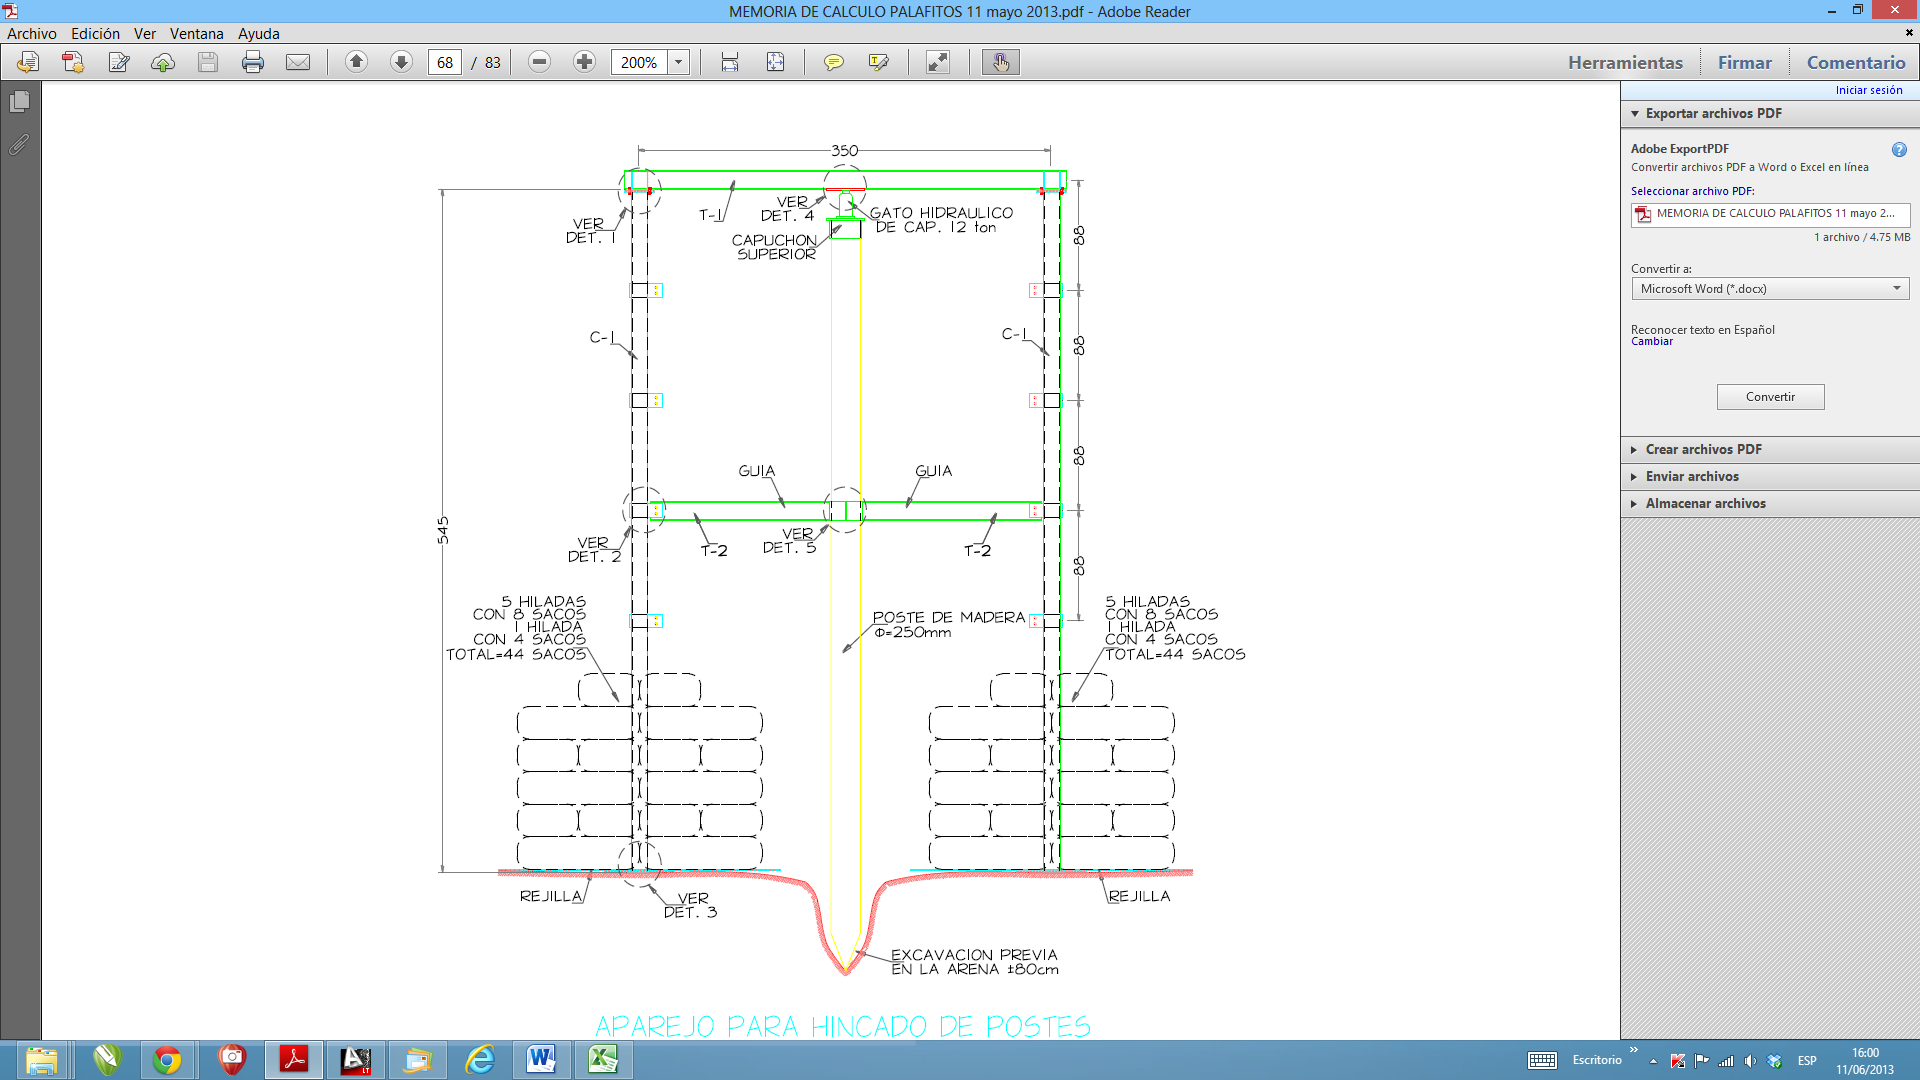
\includegraphics{texto-img/texto-img005.png}
\end{center}
\begin{center}
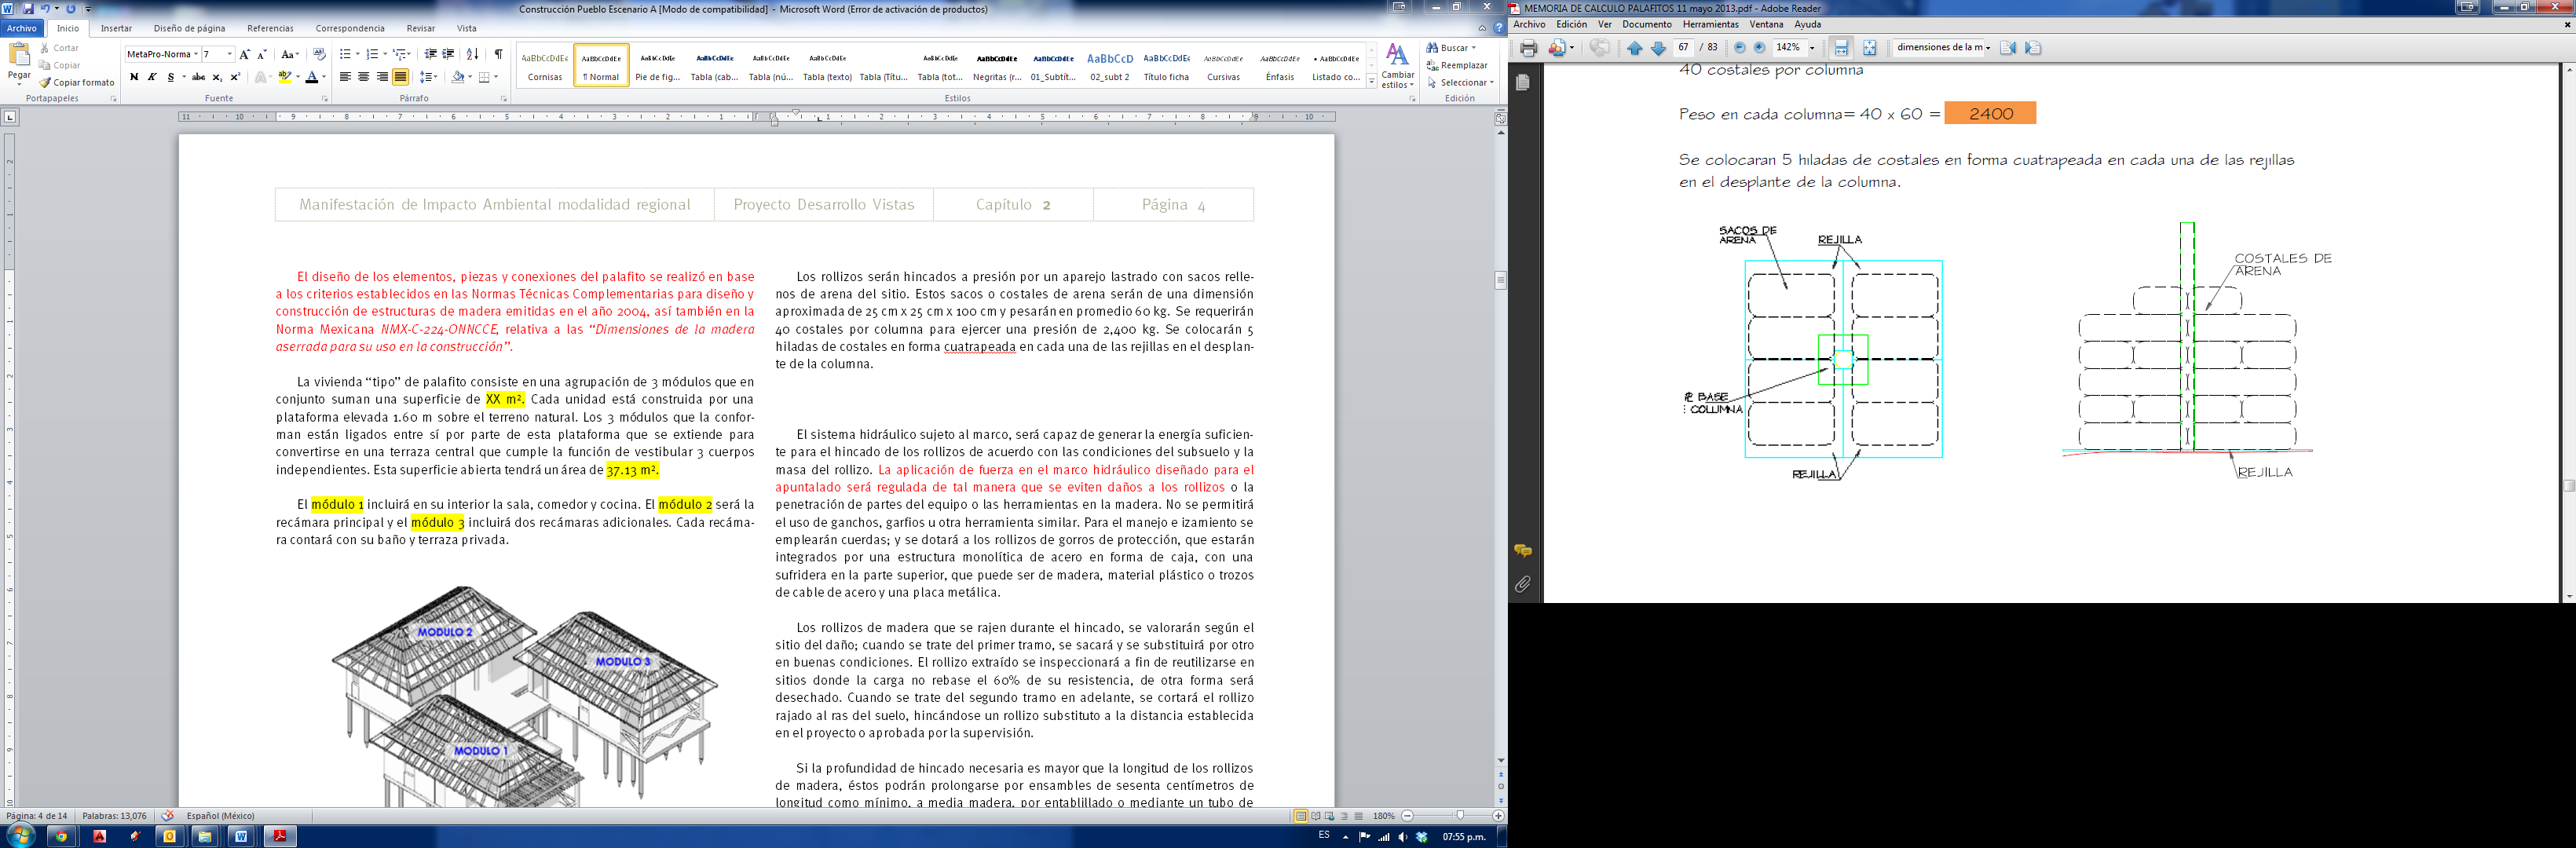
\includegraphics{texto-img/texto-img006.png}
\end{center}
\begin{center}
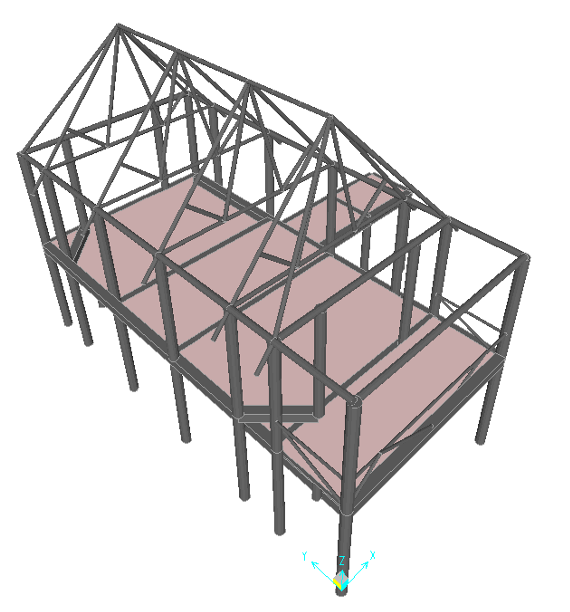
\includegraphics{texto-img/texto-img007.png}
\end{center}
\begin{center}
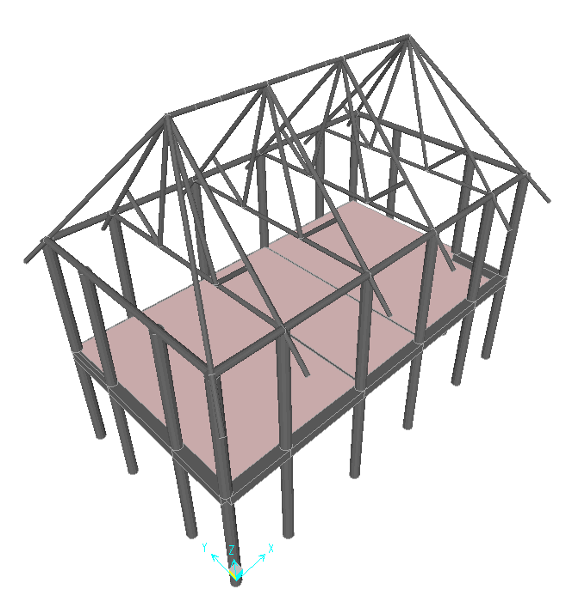
\includegraphics{texto-img/texto-img008.png}
\end{center}
\begin{center}
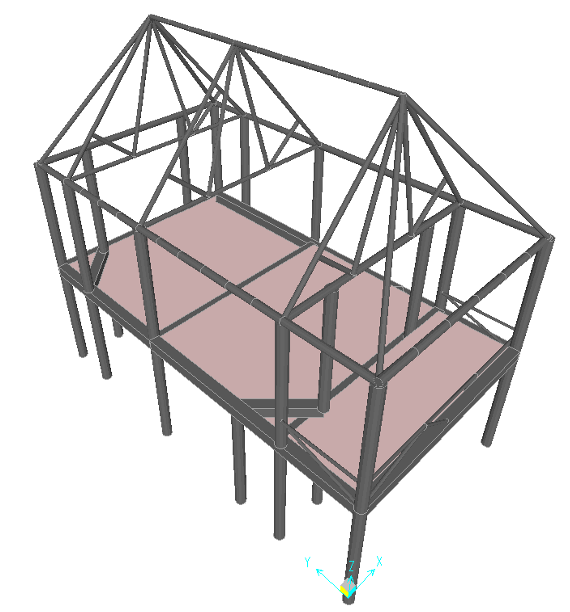
\includegraphics{texto-img/texto-img009.png}
\end{center}
\begin{center}
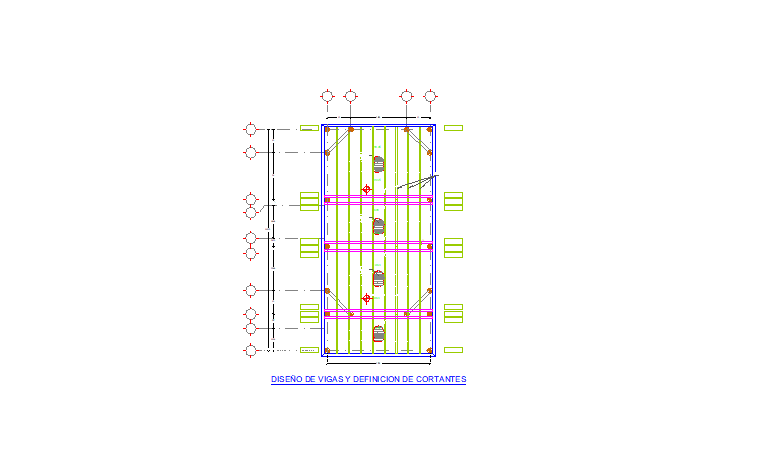
\includegraphics{texto-img/texto-img010.png}
\end{center}
\begin{center}
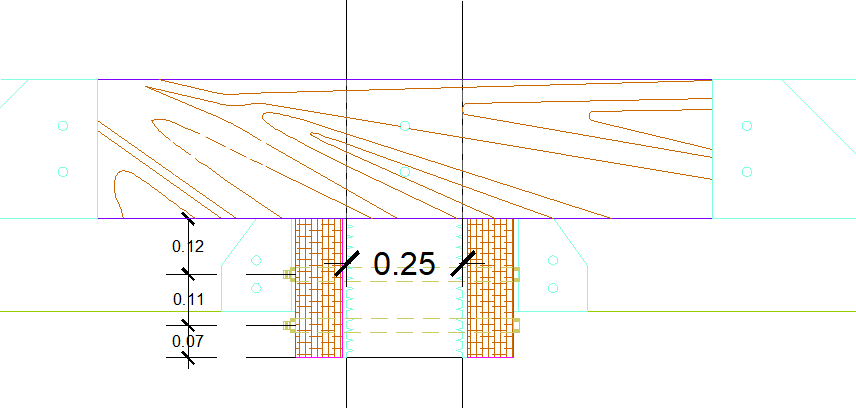
\includegraphics{texto-img/texto-img011.png}
\end{center}
\begin{center}
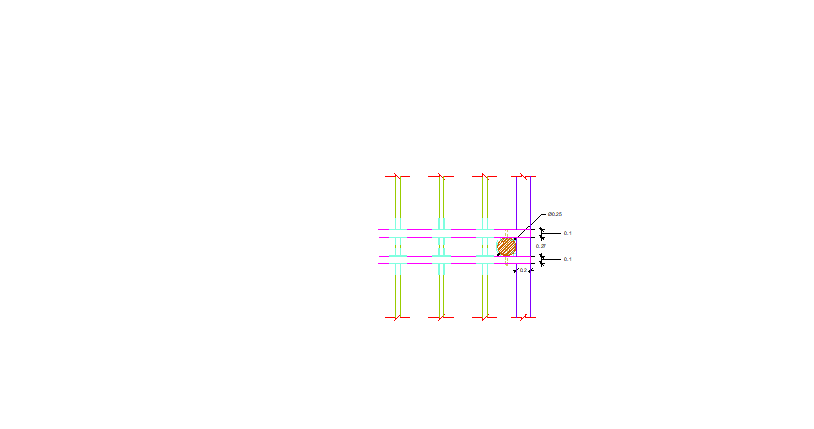
\includegraphics{texto-img/texto-img012.png}
\end{center}
\begin{center}
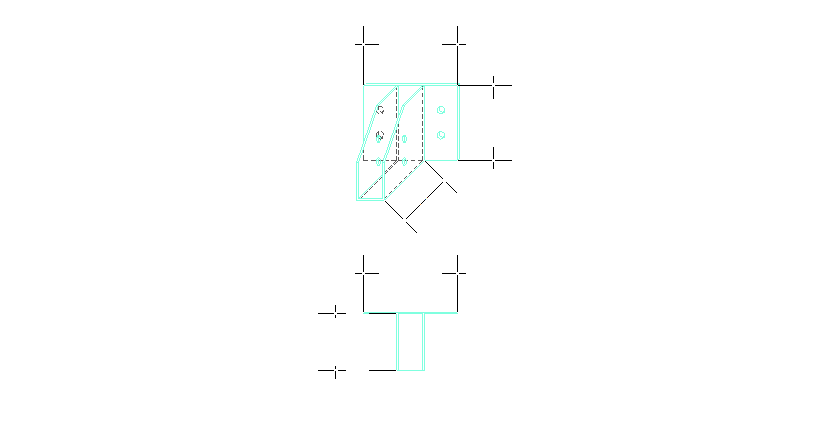
\includegraphics{texto-img/texto-img013.png}
\end{center}
\begin{center}
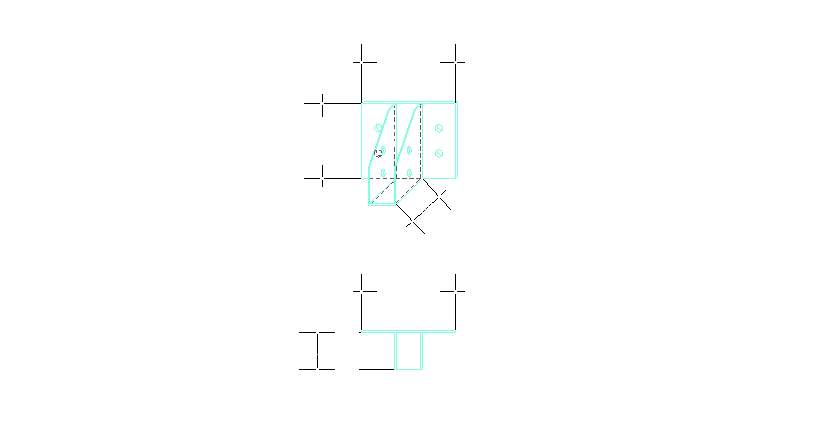
\includegraphics{texto-img/texto-img014.png}
\end{center}
\begin{center}
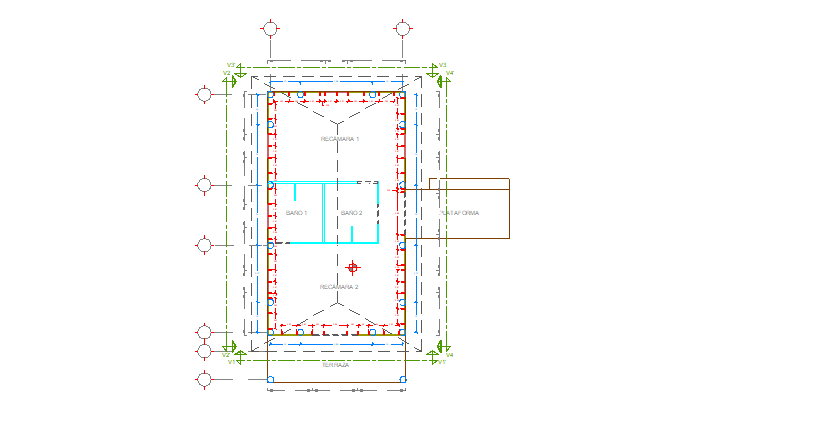
\includegraphics{texto-img/texto-img015.png}
\end{center}
\begin{center}
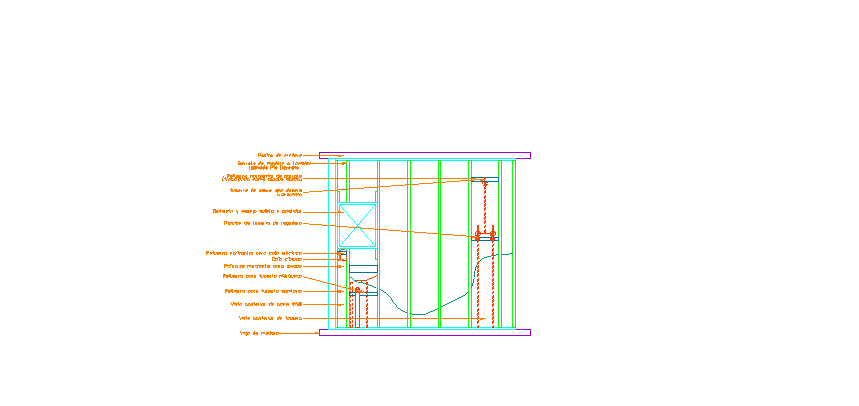
\includegraphics{texto-img/texto-img016.png}
\end{center}
\begin{center}
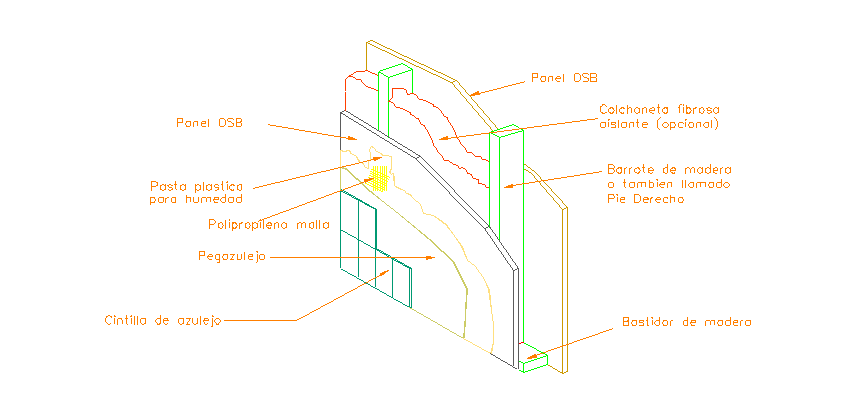
\includegraphics{texto-img/texto-img017.png}
\end{center}
\begin{center}
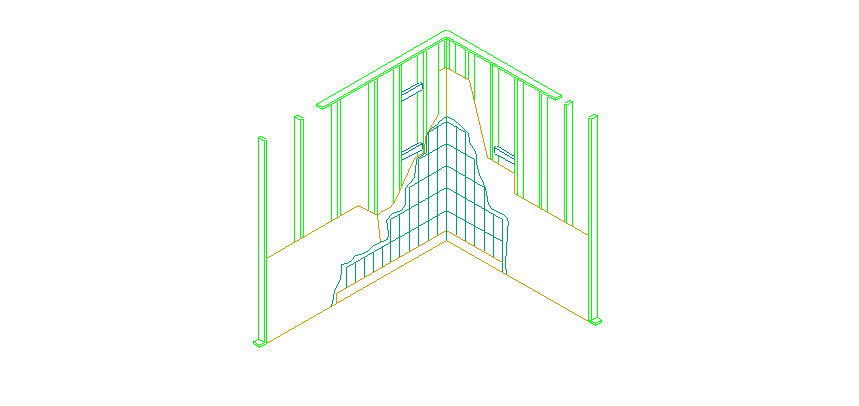
\includegraphics{texto-img/texto-img018.png}
\end{center}
\begin{center}
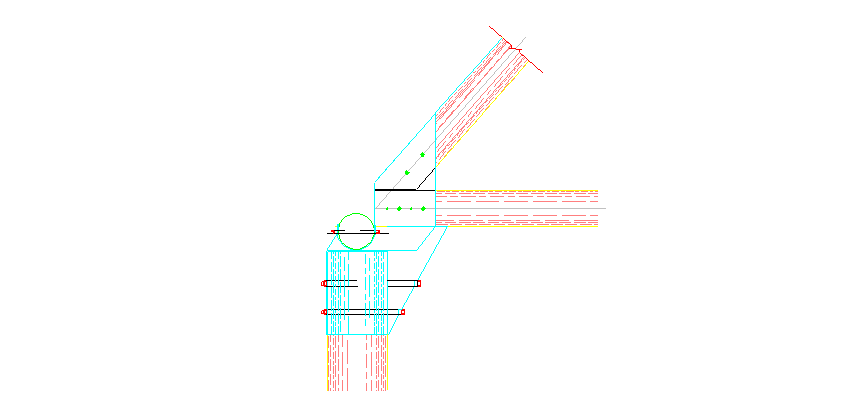
\includegraphics{texto-img/texto-img019.png}
\end{center}
\begin{center}
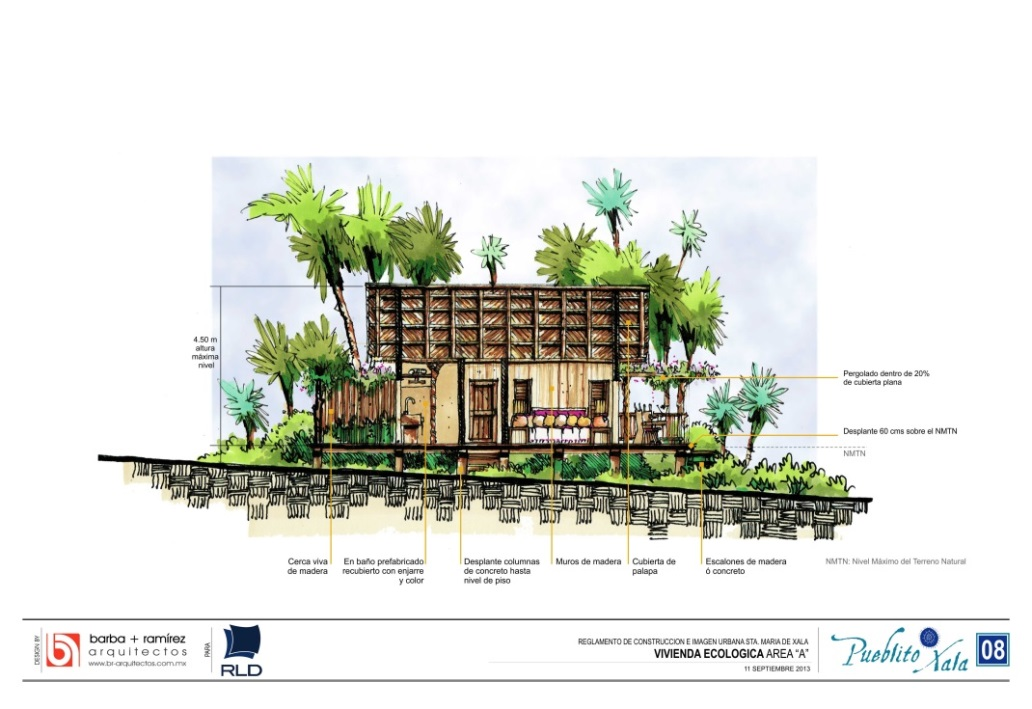
\includegraphics{texto-img/texto-img020.jpg}
\end{center}
\begin{center}
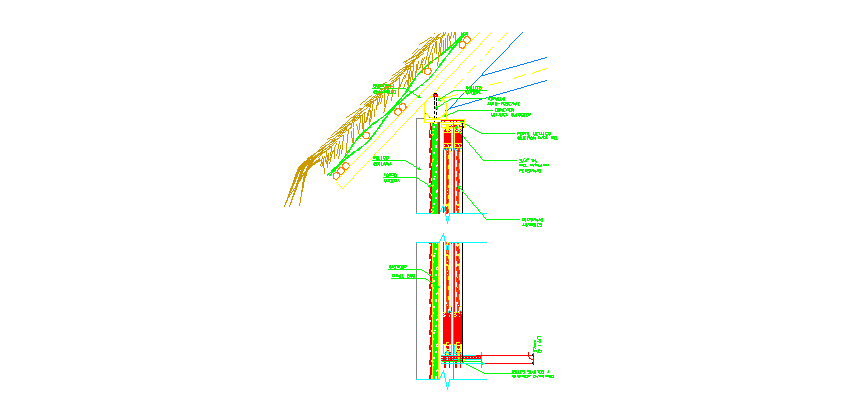
\includegraphics{texto-img/texto-img021.png}
\end{center}
\begin{center}
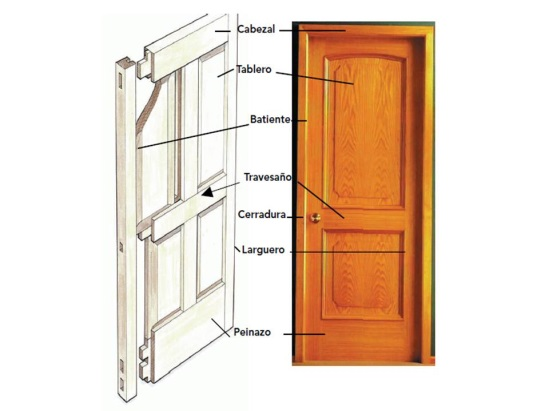
\includegraphics{texto-img/texto-img022.jpg}
\end{center}
\begin{center}
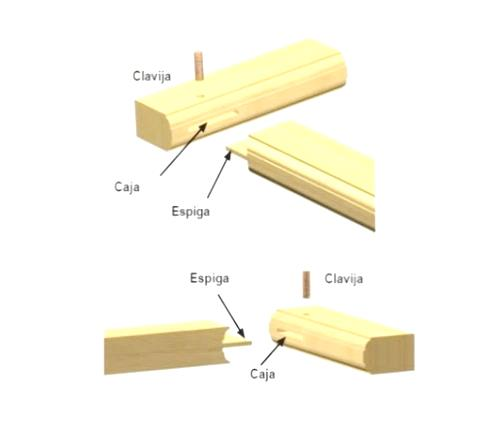
\includegraphics{texto-img/texto-img023.jpg}
\end{center}
\begin{center}
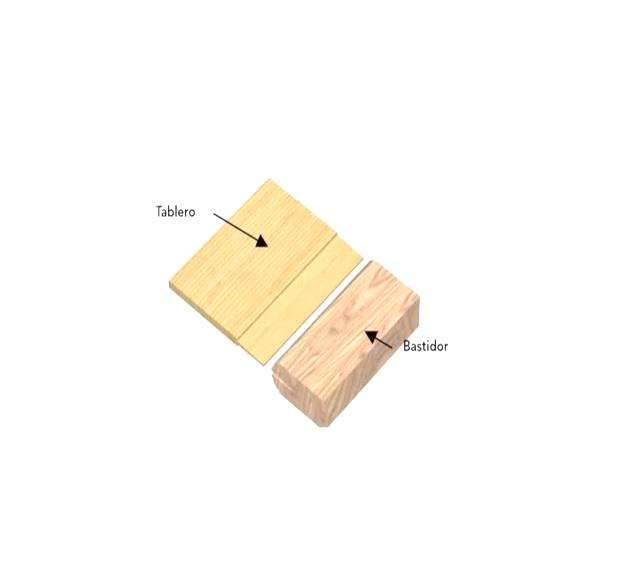
\includegraphics{texto-img/texto-img024.jpg}
\end{center}
\begin{center}
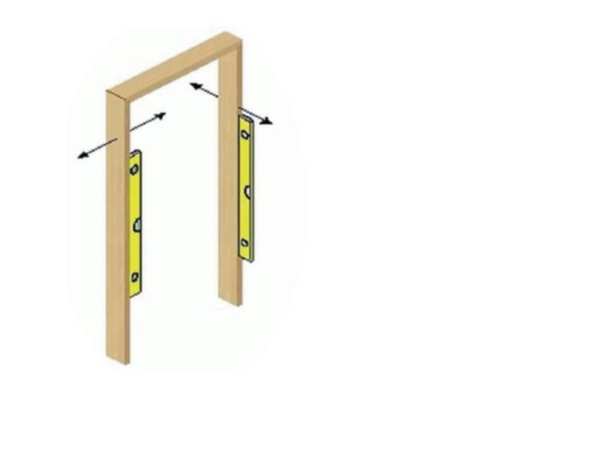
\includegraphics{texto-img/texto-img025.jpg}
\end{center}
\begin{center}
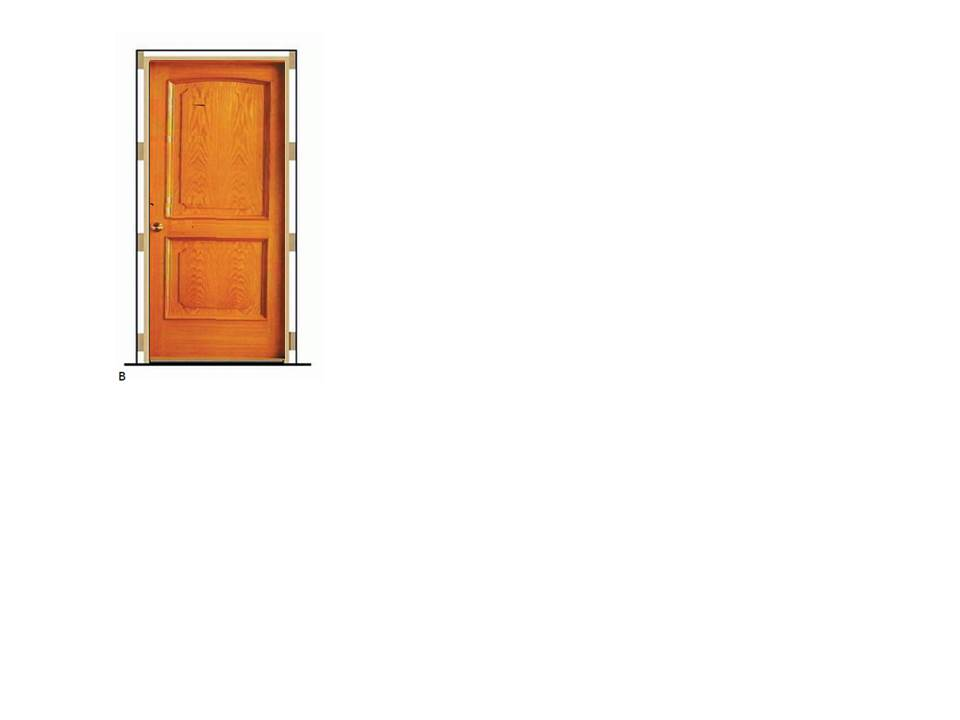
\includegraphics{texto-img/texto-img026.jpg}
\end{center}
\begin{center}
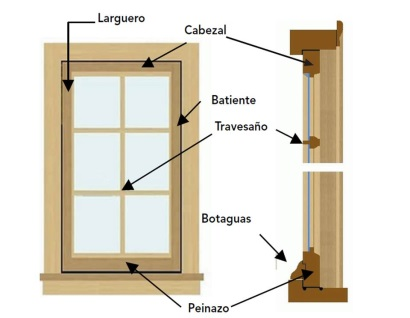
\includegraphics{texto-img/texto-img027.jpg}
\end{center}
\begin{center}
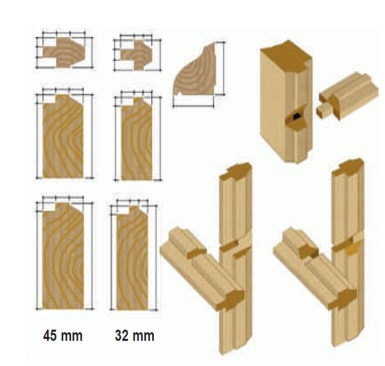
\includegraphics{texto-img/texto-img028.jpg}
\end{center}
\begin{center}
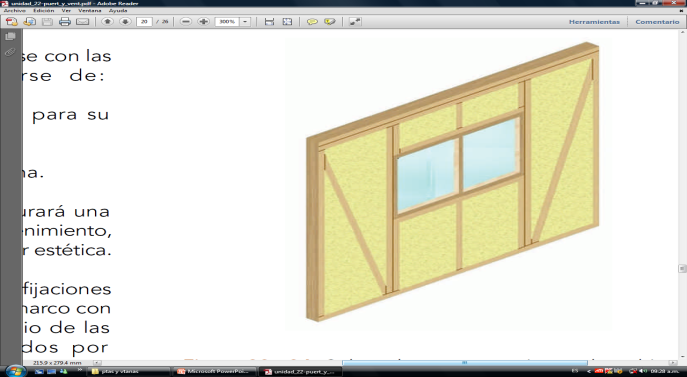
\includegraphics{texto-img/texto-img029.png}
\end{center}
\begin{center}
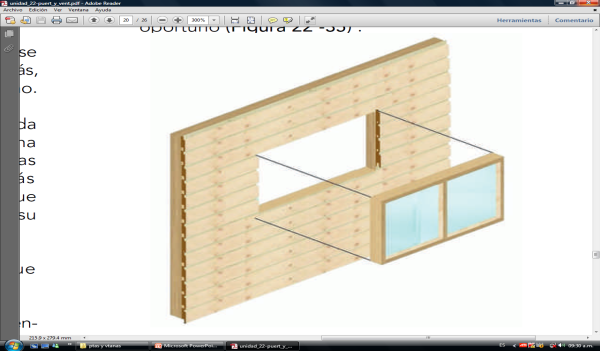
\includegraphics{texto-img/texto-img030.png}
\end{center}
\begin{center}
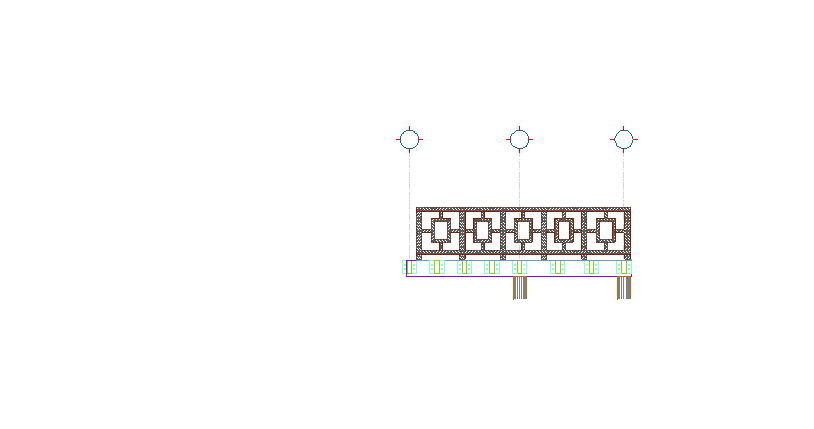
\includegraphics{texto-img/texto-img031.png}
\end{center}
\begin{center}
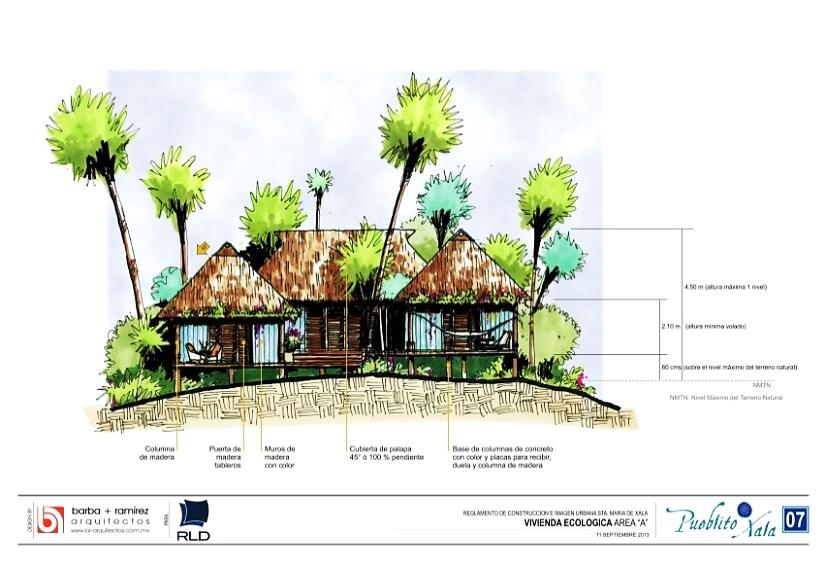
\includegraphics{texto-img/texto-img032.jpg}
\end{center}
\begin{center}
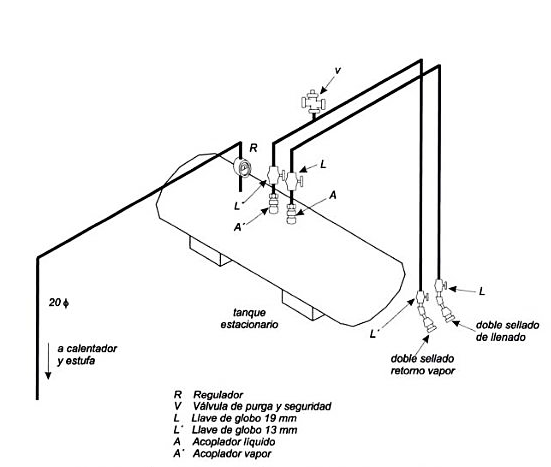
\includegraphics{texto-img/texto-img033.png}
\end{center}
\begin{center}
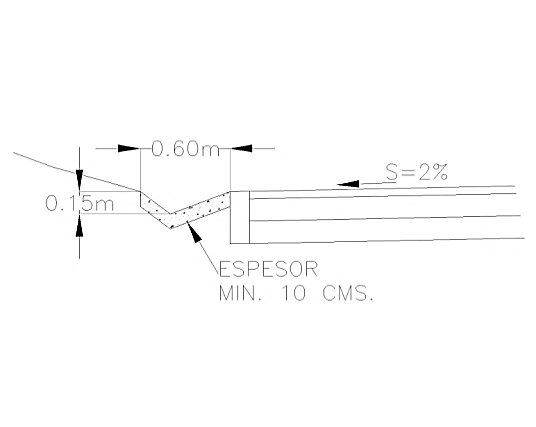
\includegraphics{texto-img/texto-img034.png}
\end{center}
\begin{center}
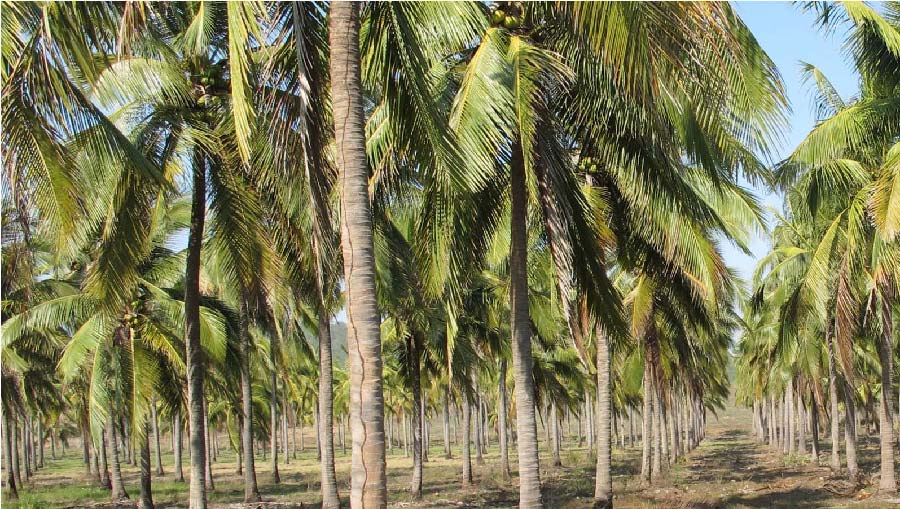
\includegraphics{texto-img/texto-img035.jpg}
\end{center}
\begin{center}
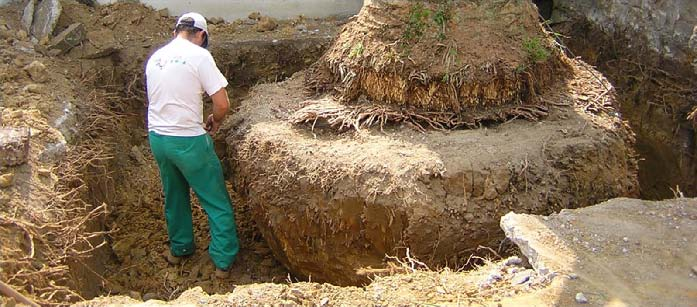
\includegraphics{texto-img/texto-img036.jpg}
\end{center}
\begin{center}
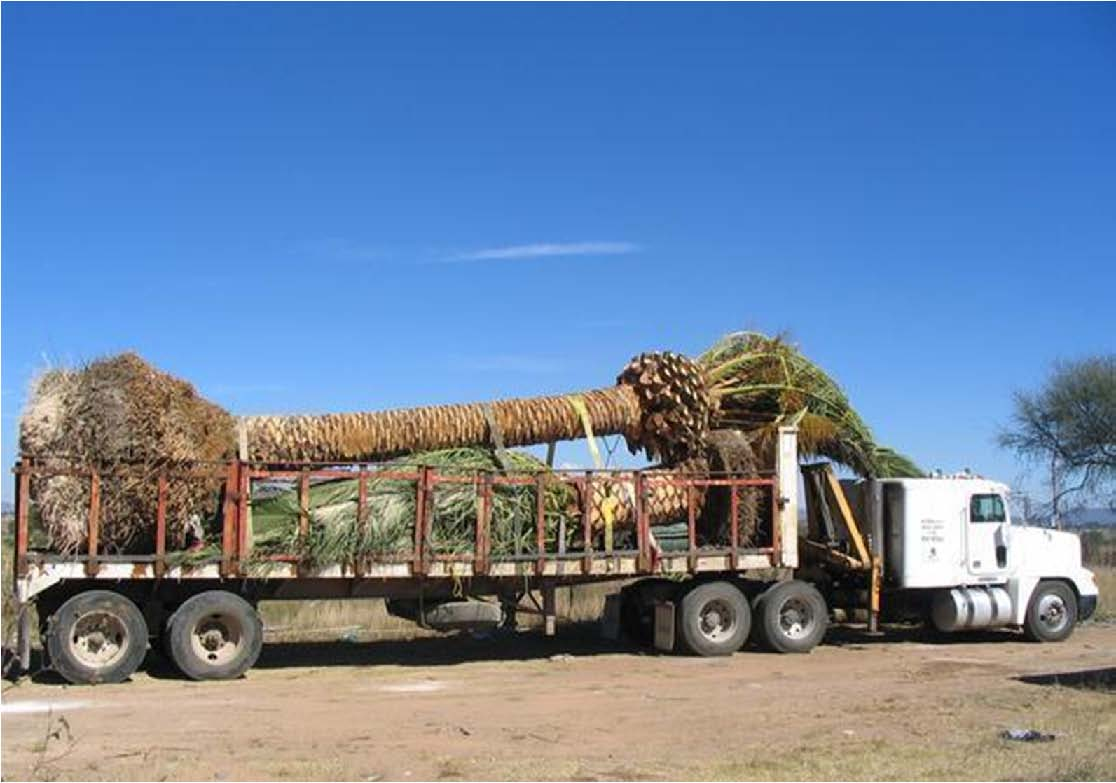
\includegraphics{texto-img/texto-img037.jpg}
\end{center}
\begin{center}
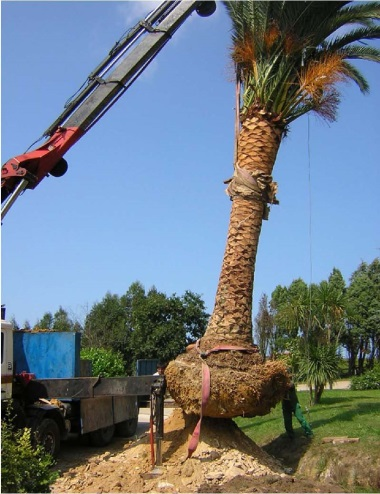
\includegraphics{texto-img/texto-img038.jpg}
\end{center}
\title{Pueblo}
\maketitle
 &
~
 &
\title{Clave: PUEB}
\maketitle
 &
~
 &
\title{Fase:}
\maketitle
 &
\title{1}
\maketitle
 &
~
 &
~
 &
~
 &
~
 &
~
 &
~
\\\hhline{-~-~~------~}
 &
~
 &
 &
~
 &
\multicolumn{1}{m{0.694cm}|}{Años: } &
\multicolumn{1}{m{0.693cm}|}{\centering 1-5} &
\multicolumn{1}{m{0.693cm}|}{\centering 6-10} &
\multicolumn{1}{m{0.693cm}|}{\centering 11-15} &
\multicolumn{1}{m{0.693cm}|}{\centering 16-20} &
\multicolumn{1}{m{0.691cm}|}{\centering 21-25} &
\multicolumn{1}{m{0.693cm}|}{\centering 26-30} &
~
\\\hhline{~~-~~------~}
 &
~
 &
\title{Construcción}
\maketitle
 &
~
 &
\multicolumn{8}{m{6.953cm}}{Duración de la obra o actividad: 1,457 días en 5 años}\\\hhline{~~-~~~~~~~~~}
\end{supertabular}
\end{flushleft}

\bigskip


\bigskip


\bigskip

\begin{multicols}{2}

\bigskip

Localización


\bigskip

 \includegraphics{texto-img/texto-img001.jpg} 


\bigskip


\bigskip

Categorías del POEL: Duna embrionaria (DEM); dunas terciarias/vegetación forestal (DTF); dunas terciarias/cobertura no forestal (DTN); dunas terciarias/vegetación secundaria de selva (DTS); primer cordón de dunas (PCD); selva baja caducifolia (SBC); vegetación forestal (VFO); cobertura no forestal (CNF); vegetación secundaria de selva (VSS).


\bigskip


\bigskip

Descripción general del componente para esta fase


\bigskip

El componente “Pueblo” se construirá a lo largo de dos fases (años 1 al 10) e integrará edificaciones relacionadas con actividades hoteleras y residenciales, actividades sociales, deportivas, artísticas y culturales, actividades comerciales y de servicios, pesca y venta de productos frescos del mar.

La fase 1 incluirá la construcción de dos hoteles boutique así como múltiples villas residenciales para alojar a visitantes (véase la tabla Construcción de producto inmobiliario para esta fase), familias de pescadores locales, trabajadores y operadores del condominio. Para las actividades comerciales y de servicios se construirán 25 edificaciones consistentes en tres restaurantes, cuatro mercados de misceláneos y productos del mar, siete comercios de productos diversos, una capilla, un módulo de escamoche, almacén y lavado de pescado, dos bodegas de refrigeración, un módulo de baños públicos y bodega, cinco establecimientos de servicios varios tales como un consultorio de atención médica de primer contacto, delegación municipal, una lavandería y dos oficinas. Para las actividades recreativas y culturales, en esta fase se construirá un gimnasio. Se construirá un estacionamiento para facilitar el ingreso a los hoteles boutique y áreas aledañas. 

La totalidad de las edificaciones de este componente se clasificarán en dos sistemas constructivos: palafitos y edificación convencional (ver sistemas constructivos al final de este apartado), y respetarán una altura máxima de 8 m o dos niveles (incluyendo la planta baja y tomando en cuenta la altura a nivel de piso natural) para mantener la visibilidad hacia la costa; de acuerdo a lo que establece el POEL en relación a las edificaciones que se ubiquen a una distancia menor a 200 m de la Zona Federal Marítimo Terrestre.

La ubicación donde se desplantará este componente coincide con la actual localización del punto público de acceso vehicular a la playa, en donde existe un asentamiento humano de familias de pescadores conformado por seis palapas o enramadas, donde viven itinerantemente alrededor de 12 familias (ver Medidas de responsabilidad social). 

Además, en este sitio se encuentra la infraestructura que actualmente alberga las instalaciones del Campamento de Conservación de Tortugas Marinas administrado por la Comisión Nacional de Áreas Naturales Protegidas (CONANP) en Chalacatepec. Dicha infraestructura será remplazada por instalaciones nuevas y diseñada de acuerdo al programa de necesidades apegado a los requerimientos de la normatividad ambiental vigente; para tal efecto, será necesario demoler las actuales (ver Demolición de las instalaciones del actual Campamento Tortuguero) y el Campamento será reubicado con la finalidad de mejorar las condiciones constructivas y operativas de las actuales instalaciones. 

Además de la superficie edificable, como parte de las áreas exteriores del componente se construirán vialidades secundarias y estacionamientos de empedrado asentado en arena (ver Sistema constructivo de vialidades secundarias convencionales); terrazas y explanadas, áreas verdes ornamentales y deportivas, dos albercas y diversos andadores de acceso al mar; todo esto empleando sistemas constructivos convencionales. 

Se construirán las redes secundarias de infraestructura hidráulica, sanitaria y de agua tratada requeridas para garantizar el abastecimiento de agua potable y la conducción del agua residual hacia su proceso de tratamiento, y desde el mismo, de vuelta a su origen para ser reutilizada en el riego de áreas verdes ornamentales. El componente cuenta con su propia Planta de Tratamiento al interior del mismo (ver componente Plantas de Tratamiento de aguas residuales y manejo de aguas residuales) y una línea de descarga de excedentes de agua tratada hasta un estanque artificial.

Se construirán además las obras secundarias de infraestructura eléctrica de baja tensión y de telecomunicaciones. La siguiente tabla muestra la totalidad de las redes de infraestructura a implementarse en esta fase.


\bigskip


\bigskip

\begin{flushleft}
\begin{tabular}{|m{1.823cm}m{2.277cm}|m{0.99799997cm}|m{0.999cm}|}

\hhline{-~~~}
\multicolumn{1}{|m{1.823cm}|}{\centering Longitudes de infraestructura a implementar por categoría del POEL (km)} &
\\\hline
\multicolumn{2}{|m{4.3cm}|}{\centering Tipo de red} &
\centering VFO &
\centering\arraybslash DTF\\\hline
\multicolumn{2}{|m{4.3cm}|}{Hidráulica} &
\centering 1.4 &
\centering\arraybslash 0.3\\\hline
\multicolumn{2}{|m{4.3cm}|}{Sanitaria} &
\centering 1.4 &
\centering\arraybslash 0.4\\\hline
\multicolumn{2}{|m{4.3cm}|}{Agua tratada} &
\centering 1.6 &
\centering\arraybslash 0.4\\\hline
\multicolumn{2}{|m{4.3cm}|}{Telecomunicaciones} &
\centering 1.2 &
\centering\arraybslash 0.6\\\hline
\multicolumn{2}{|m{4.3cm}|}{Eléctrica aérea} &
\centering 0.2 &
\centering\arraybslash 0\\\hline
\multicolumn{2}{|m{4.3cm}|}{Eléctrica subterránea} &
\centering 1.0 &
\centering\arraybslash 0.5\\\hline
\end{tabular}
\end{flushleft}

\bigskip


\bigskip

Previo al inicio de los procesos de obra, las actividades del componente incluyen la construcción de edificaciones de carácter provisional denominadas Obras temporales, las cuales se ubicarán en la brecha existente que bordea el componente al límite sureste así como en el sitio donde será la explanada central del componente el cual presenta Cobertura No Forestal; dichos espacios tendrán la finalidad de servir como áreas auxiliares de trabajo y almacenamiento desde donde los trabajadores se desplazarán al lugar de trabajo correspondiente. Estas obras no formarán parte del componente pero son necesarias para albergar de forma temporal trabajadores, insumos, maquinaria, equipos, etc.; y serán retiradas una vez concluida la totalidad del componente al término de la fase 2.


\bigskip


\bigskip

\begin{flushleft}
\begin{tabular}{|m{4.349cm}m{1.749cm}|}

\hhline{-~}
\multicolumn{1}{|m{4.349cm}|}{\centering Datos generales del componente para esta fase} &
\\\hline
\multicolumn{2}{|m{6.298cm}|}{Superficie aprovechable total (ha)}\\\hline
\multicolumn{2}{|m{6.298cm}|}{Superficie edificable (ha)}\\\hline
\multicolumn{2}{|m{6.298cm}|}{Superficie a construir no edificable (ha)}\\\hline
\multicolumn{2}{|m{6.298cm}|}{Macrolotes del plan maestro}\\\hline
\multicolumn{2}{|m{6.298cm}|}{UGA POEL}\\\hline
\multicolumn{2}{|m{6.298cm}|}{Niveles máximos construidos}\\\hline
\multicolumn{2}{|m{6.298cm}|}{Cuartos totales construidos}\\\hline
\end{tabular}
\end{flushleft}

\bigskip


\bigskip

\begin{flushleft}
\begin{tabular}{|m{1.0999999cm}m{0.05600001cm}|m{1.084cm}|m{0.984cm}|m{1.134cm}|m{1.01cm}|m{0.86200005cm}|}

\hhline{-~~~~~~}
\multicolumn{1}{|m{1.0999999cm}|}{\centering Tipos de aprovechamiento por cobertura para esta fase } &
\\\hline
\multicolumn{2}{|m{1.356cm}|}{\centering Categorías del POEL} &
\centering Cobertura del suelo &
\centering Superficie edificable (ha) &
\multicolumn{3}{m{3.4060001cm}|}{\centering Sup. a construir no edificable (ha)}\\\hline
 &
 &
 &
 &
\centering Terrazas, patios, explanadas, andadores &
\centering Vialidades internas &
\centering\arraybslash Albercas\\\hline
\multicolumn{2}{|m{1.356cm}|}{Vegetación forestal } &
Matorral crasicaule &
\raggedleft 0.32 &
\raggedleft 1.26 &
\raggedleft 0.89 &
\raggedleft\arraybslash 0.02\\\hline
 &
 &
Matorral espinoso costero &
\raggedleft 0.23 &
\raggedleft 0.39 &
\raggedleft 0.09 &
\raggedleft\arraybslash 0\\\hline
\multicolumn{2}{|m{1.356cm}|}{Duna Terciaria Vegetación forestal } &
Matorral crasicaule &
\raggedleft 0.05 &
\raggedleft 0.37 &
\raggedleft 0.18 &
\raggedleft\arraybslash 0\\\hline
 &
 &
Matorral espinoso costero &
\raggedleft 0.44 &
\raggedleft 1.37 &
\raggedleft 0.13 &
\raggedleft\arraybslash 0.01\\\hline
\multicolumn{2}{|m{1.356cm}|}{Duna Terciaria Cobertura no forestal } &
Cobertura alterada &
\raggedleft 0 &
\raggedleft 0.01 &
\raggedleft 0 &
\raggedleft\arraybslash 0\\\hline
\multicolumn{2}{|m{1.356cm}|}{Cobertura no forestal } &
Cobertura alterada &
\raggedleft 0.24 &
\raggedleft 0.59 &
\raggedleft 0.13 &
\raggedleft\arraybslash 0.01\\\hline
\end{tabular}
\end{flushleft}

\bigskip


\bigskip

\begin{flushleft}
\begin{tabular}{|m{1.62cm}m{0.83cm}|m{2.3009999cm}|m{1.2989999cm}|m{1.051cm}|}

\hhline{-~~~~}
\multicolumn{1}{|m{1.62cm}|}{\centering Construcción de producto inmobiliario para esta fase} &
\\\hline
\multicolumn{2}{|m{2.6499999cm}|}{\centering Categorías del POEL} &
\centering Cobertura del suelo &
\multicolumn{2}{m{2.55cm}|}{\centering Número de cuartos}\\\hline
 &
 &
 &
\centering Hoteleros &
\centering\arraybslash Villas*\\\hline
\multicolumn{2}{|m{2.6499999cm}|}{Vegetación forestal } &
Matorral crasicaule &
\raggedleft 11 &
\raggedleft\arraybslash 18\\\hline
 &
 &
Matorral espinoso costero &
\raggedleft 11 &
\raggedleft\arraybslash 0\\\hline
\multicolumn{2}{|m{2.6499999cm}|}{Duna Terciaria Vegetación forestal } &
Matorral crasicaule &
\raggedleft 0 &
\raggedleft\arraybslash 0\\\hline
 &
 &
Matorral espinoso costero &
\raggedleft 40 &
\raggedleft\arraybslash 10\\\hline
\multicolumn{2}{|m{2.6499999cm}|}{Duna Terciaria Cobertura no forestal } &
Cobertura alterada &
\raggedleft 0 &
\raggedleft\arraybslash 0\\\hline
\multicolumn{2}{|m{2.6499999cm}|}{Cobertura no forestal } &
Cobertura alterada &
\raggedleft 18 &
\raggedleft\arraybslash 0\\\hline
\multicolumn{5}{|m{7.901cm}|}{\raggedleft Gran Total}\\\hline
\end{tabular}
\end{flushleft}
* Una villa equivale a 2.5 cuartos hoteleros


\bigskip


\bigskip

Descripción de las obras y actividades del componente para esta fase


\bigskip

Este componente implementará doce procesos constructivos con base en la vulnerabilidad del ecosistema y el tipo de obra. Los procesos constructivos se describen a continuación.


\bigskip


\bigskip

\begin{flushleft}
\begin{tabular}{m{2.7949998cm}m{0.26cm}|m{3.899cm}|}
\hhline{-~~}
\multicolumn{1}{|m{2.7949998cm}|}{\centering Implementación de procesos constructivos por tipo de ecosistema para esta fase} &
\\\hline
\multicolumn{2}{|m{3.2549999cm}|}{\centering Proceso constructivo} &
\centering\arraybslash Categoría del POEL\\\hline
\multicolumn{2}{|m{3.2549999cm}|}{Palafitos} &
Vegetación forestal\\\hline
 &
 &
Duna Terciaria Vegetación forestal\\\hhline{~~-}
 &
 &
Duna Terciaria Cobertura no forestal\\\hhline{~~-}
 &
 &
Cobertura no forestal\\\hline
\multicolumn{2}{|m{3.2549999cm}|}{Edificaciones convencionales} &
Vegetación forestal\\\hline
 &
 &
Duna Terciaria Vegetación forestal\\\hhline{~~-}
 &
 &
Cobertura no forestal\\\hline
\multicolumn{2}{|m{3.2549999cm}|}{Vialidades secundarias} &
Vegetación forestal\\\hline
 &
 &
Duna Terciaria Vegetación forestal\\\hhline{~~-}
 &
 &
Cobertura no forestal\\\hline
\multicolumn{2}{|m{3.2549999cm}|}{Albercas convencionales} &
Duna Terciaria Vegetación forestal \\\hline
 &
 &
Cobertura no forestal\\\hline
\multicolumn{2}{|m{3.2549999cm}|}{Cuerpo de agua artificial} &
Vegetación forestal \\\hline
\multicolumn{2}{|m{3.2549999cm}|}{Áreas verdes ornamentales} &
Vegetación forestal \\\hline
 &
 &
Duna Terciaria Vegetación forestal \\\hhline{~~-}
 &
 &
Duna Terciaria Cobertura no forestal\\\hhline{~~-}
 &
 &
Cobertura no forestal\\\hline
\multicolumn{2}{|m{3.2549999cm}|}{Terrazas, patios y explanadas} &
Vegetación forestal\\\hline
 &
 &
Duna Terciaria Vegetación forestal \\\hhline{~~-}
 &
 &
Duna Terciaria Cobertura no forestal\\\hhline{~~-}
 &
 &
Cobertura no forestal\\\hline
\multicolumn{2}{|m{3.2549999cm}|}{Instalación hidrosanitaria y de agua tratada secundaria} &
Vegetación forestal \\\hline
 &
 &
Duna Terciaria Vegetación forestal\\\hhline{~~-}
 &
 &
Duna Terciaria Cobertura no forestal\\\hhline{~~-}
 &
 &
Cobertura no forestal\\\hline
\multicolumn{2}{|m{3.2549999cm}|}{Instalación eléctrica aérea secundaria} &
Vegetación forestal\\\hline
 &
 &
Cobertura no forestal \\\hline
\multicolumn{2}{|m{3.2549999cm}|}{Instalación eléctrica y de telecomunicaciones subterránea secundaria} &
Vegetación forestal \\\hline
 &
 &
Duna Terciaria Vegetación forestal\\\hhline{~~-}
 &
 &
Cobertura no forestal \\\hline
\multicolumn{2}{|m{3.2549999cm}|}{Demolición de Campamento Tortuguero actual} &
Cobertura no forestal \\\hline
\multicolumn{2}{|m{3.2549999cm}|}{Obras provisionales temporales~} &
Cobertura no forestal \\\hline
\end{tabular}
\end{flushleft}

\bigskip
\end{multicols}
Proceso constructivo de edificación tipo Palafitos 


\bigskip

Colocación de señalización preventiva y restrictiva.

Colocación de tambos de 200 L para residuos.

Trazo, limpieza y desmonte en las áreas donde sea necesario.

Preparación de la superficie para la colocación del marco hidráulico apuntalador (Ver sistema constructivo Palafito).

Perforación previa al hincado de rollizos con pico y pala.

Colocación del marco hidráulico apuntalador. 

Suministro de elemento estructural denominado rollizo de madera (CM).

Revisión y paso de control de calidad de la madera a utilizar (previamente secada y libre de cualquier daño estructural).

Hincado a presión de rollizos de madera por un aparejo lastrado con sacos rellenos de arena proveniente de bancos autorizados. 

Reincorporación al suelo del material producto de la perforación previa.

Habilitado de plataforma que forma el piso de duela de primera de 1”~×~3” ×~8 pies a base de elementos estructurales denominados vigas secundarias (T-P) apoyadas sobre vigas madrinas interiores (T-D’) y exteriores (T-D) para formar un diagrama rígido.

Suministro e instalación de elemento estructural en muro perimetral y divisorio denominado barrote de 0.04~×~0.10~×~2.40 m.

Suministro e instalación de elemento estructural en muro perimetral denominado barrote de 0.04~×~0.10~×~1.20 m.

Suministro e instalación de elemento estructural en muro perimetral denominado barrote de 0.04~×~0.10~×~0.90 m.

Suministro e instalación de forro de muro exterior de madera Chiche (Aspidosperma megalocarpon) de 2” ×~4” ×~8 pies sobre elementos estructurales denominados barrotes.

Instalación de forro de muro interior de panel OSB de 1.22~×~2.44~×~0.19 m forrado con malla de polipropileno y pasta tipo base coat.

Instalación de azulejo de 0.20~×~0.20 m en muros y pisos de baños, así como muros de cocina.

Colocación de ductos y tuberías de la instalación hidrosanitaria suspendidas al lecho bajo de las vigas y pisos.

Colocación de ductos, tuberías y cableado de la instalación eléctrica suspendidas al lecho bajo de las vigas y pisos.

Colocación de cilindro de gas de 30 kg con tuberías de cobre.

Colocación del sistema de iluminación interior y exterior conforme a las especificaciones generales de la Norma Oficial Mexicana NOM-162-SEMARNAT-2012.

Suministro e instalación de elemento estructural sobre muro perimetral denominado rollizo corona (T-C).

Suministro e instalación de armadura de madera de chiche (Aspidosperma megalocarpon) para asentar y fijar la cubierta. 

Fabricación e instalación de cubierta tipo palapa, de hoja de palma real (Sabal Mexicana) previamente tratada; armado y entramado de la estructura de la palapa a base de madera de guayabillo (Lasiocarpus ferrugineus).

Fabricación e instalación de escalera de madera de chiche (Aspidosperma megalocarpon).

Fabricación e instalación de barandal de madera Chiche (Aspidosperma megalocarpon) 2”x2”x0.90 m. 

Suministro e instalación de puertas de tablero para exterior de madera de parota o huanacaxtle (Enterolobium cyclocarpum).

Suministro e instalación de ventanas de madera de parota o huanacaxtle.

Suministro y colocación de elementos ornamentales en madera (pergolados).

Colocación del equipo necesario para el funcionamiento de las instalaciones y realización de pruebas de puesta en servicio.

Limpieza general. 

Traslado de material de escombro al sitio autorizado para su depósito.


\bigskip


\bigskip

Proceso constructivo de edificaciones convencionales


\bigskip

Colocación de señalización preventiva y restrictiva.

Colocación de tambos de 200 L como contenedores para residuos.

Colocación de barreras físicas para impedir el impacto visual y generar ingreso controlado al sitio de la obra.

Preparación del sitio, limpieza, trazo del terreno con equipo topográfico de precisión satelital.

Apertura de brecha y desmonte, incluyendo desenraice y remoción o poda de ejemplares arbóreos y arbustivos.

Despalme con maquinaria de manera exclusiva en las áreas de aprovechamiento, excluyendo superficies que serán destinadas a áreas verdes.

Acarreo por medios mecánicos de material resultante del desmonte y despalme hasta el sitio autorizado para su alojamiento.

Excavación por medios mecánicos en cualquier material para cimentaciones y tendido de redes de infraestructura.

Nivelación y compactación de suelo por medios mecánicos al 90\% de su prueba proctor estándar.

Construcción de plantilla de concreto pobre f'c~=~100 de 5 cm de espesor en cimentación para recibir el acero de refuerzo.

Construcción de cimentación tipo zapata corrida y aislada con concreto armado f´c~=~250 kg/cm² y trabe de liga del mismo material.

Impermeabilización en cimentación para evitar que la humedad del suelo suba al muro

Construcción de redes de infraestructura eléctricas, hidráulicas y sanitarias y de gas.

Relleno con material producto de la excavación y apisonamiento.

Construcción de estructura de concreto armado con acero, incluyendo elementos como castillos, columnas, trabes, dalas de cerramiento y medianeras.

Construcción de estructura a base de elementos verticales y horizontales de madera tales como columnas, vigas y trabes.

Construcción de firmes de concreto armado con acero, resistencias según especificaciones del proyecto.

Forjado de muros de block, tabique rojo, piedra braza o de concreto armado según especificaciones del proyecto. Asentados con mortero cemento arena, de acuerdo a las especificaciones generales de obra. 

Construcción de cubiertas según especificaciones de proyecto, pudiendo ser cubierta inclinada con vigas de madera, medio pliego y teja de barro; losa plana con vigas de madera, medio pliego, capa de compresión y casetón de poliestireno; estructura metálica con triplay y teja de barro; bóveda de cañón de concreto; losa llena de concreto armado según sea el caso. 

Habilitado de canaletas y bajantes pluviales.

Construcción de escaleras con las características y dimensiones que especifique el proyecto, forjadas con tabique y/o concreto reforzado con acero.

Aplanado en muros empleando mortero cemento-arena proporción 1:5 de 2 cm de espesor acabado según especificaciones del proyecto.

Acabado en muros con pintura vinil-acrílica y recubrimiento de muros ornamentales o en interiores de baños y cocinas empleando piedra laja, cantera, mosaico veneciano, u otros según proyecto.

Colocación de recubrimiento para acabado en piso interior y exterior, incluyendo materiales pétreos como piedra laja, cantera o losetas de barro en piezas de 20~×~20 cm con juntas de 6 mm.

Impermeabilización en losa a 2 manos.

Colocación de muebles de baño y equipamiento de instalaciones (aire acondicionado, gas, calderas y otros equipos que se requieran).

Colocación de acabados de carpintería, herrería, cancelería.

Limpieza general y separación de residuos según los procedimientos de ley.

Traslado de material de escombro al sitio autorizado para su depósito.


\bigskip


\bigskip

Proceso constructivo de vialidades de empedrado asentado en arena


\bigskip

Colocación de señalización preventiva y restrictiva.

Colocación de tambos de 200 L como contenedores para residuos.

Preparación del sitio, limpieza, trazo y nivelación del terreno con equipo topográfico de precisión satelital.

Apertura de brecha y desmonte, incluyendo desenraice para inicio de trabajos de movimiento de tierras por medios mecánicos; y remoción o poda de ejemplares arbóreos dentro del derecho de vía.

Despalme de capa edáfica hasta 20 cm de espesor con maquinaria de manera exclusiva en las áreas de aprovechamiento.

Acarreo por medios mecánicos de material resultante desmonte y despalme hasta el sitio autorizado para su alojamiento.

Excavación en cualquier material, hasta 0.40 m de profundidad, para conformación de subrasante y capa de base.

Nivelación y compactación de terreno natural por medios mecánicos al 90\% de su prueba proctor estándar; este proceso se repetirá entre cada una de las capas subrasante y de base que se coloquen.

Suministro y colocación de material de préstamo (proveniente de bancos de material o producto de la excavación según resultados de estudios de mecánica de suelos) para capa subrasante de 20 cm de espesor.

Colocación de base de arena fina en capas de 20 cm, escarificación de suelo para hincado de piedra.

Suministro e hincado de piedra bola de río de canto rodado asentada en la capa de arena, emporado de juntas.

Compactación y fijación de superficie de rodamiento.

Excavación en cualquier material, hasta 0.40 m de profundidad, para la conformación de la base de las cunetas pluviales.

Acarreo por medios mecánicos de material resultante de la excavación hasta el sitio autorizado para su alojamiento en las obras temporales del componente

Humedecimiento de la base, nivelación y compactación de la superficie al 90\% mediante apisonamiento manual.

Colocación de cimbra metálica a cada 3 metros.

Construcción de cuneta a base de concreto f’c 150 kg/cm² reforzado con malla electrosoldada.

Curado de concreto y retiro de cimbra.

Perfilado de cuneta y corrección de irregularidades empleando mortero cemento arena, proporciones según proyecto.

Sellado de junta fría.

Colocación de señales de alineamiento vial fantasmas de concreto a cada 20~m.

Suministro y colocación de señalizaciones de madera y elementos de iluminación de cortesía, incluye equipos y accesorios.

Limpieza general.

Traslado de material de escombro al sitio autorizado para su depósito.


\bigskip


\bigskip

Proceso constructivo de albercas convencionales


\bigskip

Colocación de señalización preventiva y restrictiva.

Colocación de tambos de 200 L como contenedores para residuos.

Preparación del sitio, limpieza, trazo y nivelación del terreno con equipo topográfico de precisión satelital.

Excavación de fosa para alberca por medios mecánicos en cualquier material.

Acarreo de material producto de la excavación en camión hasta el sitio autorizado para su alojamiento en las obras temporales.

Compactación del suelo una vez que se alcanzó el nivel de desplante, empleando medios mecánicos al 90\% de su prueba proctor estándar.

Construcción de losa de fondo y muros de concreto premezclado, resistencia según proyecto, armado con acero de refuerzo fy~=~4200 kg/cm².

Forjado de escaleras con block de jalcreto asentadas con mortero cemento-arena 1:5.

Aplanado en muros interiores de alberca con mortero cemento-arena proporción 1:5 de 2 cm de espesor acabado rústico.

Suministro y colocación de recubrimiento para muros de albercas de dimensiones 2.5x2.5 cm de mosaico tipo veneciano.

Construcción y equipamiento del cuarto de máquinas.

Limpieza general.

Traslado de material de escombro al sitio autorizado para su depósito.


\bigskip


\bigskip

Proceso constructivo de cuerpos de agua artificial (embalses)


\bigskip

Colocación de señalización preventiva y restrictiva.

Colocación de tambos de 200 L como contenedores para residuos.

Preparación del sitio, limpieza, trazo del terreno con equipo topográfico de precisión satelital.

Excavación por medios mecánicos en cualquier material.

Acarreo por medios mecánicos de material resultante de la excavación hasta el sitio autorizado para su alojamiento en las obras temporales.

Conformación de taludes con material producto de excavación, compactado al 90\% prueba proctor.

Recubrimiento de taludes con capa de 20 cm de arena de granulometría controlada como base para desplante de cuerpo de agua.

Habilitado de tubo de respiración de 4” de diámetro recubierto con malla geotextil tipo pavitex 200 o similar.

Colocación de refuerzo perimetral de cuerpos de agua con liner de triple capa conformado por: dos capas exteriores de Geomembrana de caucho sintético tipo EPDM 1.02 mm o similar y una capa central de geotextil 200 gr/m² tipo pavitex 200 o similar.

Recubrimiento de taludes con material pétreo en capas de 5 cm de espesor sin juntear ni asentar.

Habilitado de equipos de circulación de agua y accesorios.

Limpieza general.

Traslado de material de escombro al sitio autorizado para su depósito.


\bigskip


\bigskip

Proceso constructivo de áreas verdes ornamentales


\bigskip

Colocación de señalización preventiva y restrictiva.

Colocación de tambos de 200 L como contenedores para residuos.

Identificación de ejemplares a trasladar con su marca de orientación magnética y ángulo de inclinación original.

Excavación, envasado del ejemplar (palmera) y formación del cepellón.

Protección del cepellón expuesto con material biodegradable.

Limpieza y desmonte de superficie. 

Acarreo por medios mecánicos de material resultante del desmonte hasta el sitio autorizado para su alojamiento en las obras temporales.

Trazo de los sitios de plantación de ejemplares con equipo topográfico de precisión.

Excavación de cepas de 2.40 m por lado y 0.90 m de profundidad para colocación de cepellón.

Mejoramiento de capa edáfica del sitio con tierra vegetal hasta 20 cm de espesor por medios manuales y mecánicos.

Traslado y maniobra de izaje de ejemplares provenientes del palmar existente en el PDV, empleando medios mecánicos.

Colocación del ejemplar cuidando que mantenga su orientación e inclinación original.

Relleno de cepa con material del sitio y compactación con equipo manual.

Suministro y colocación de vegetación ornamental endémica para el estrato bajo, medio y alto proveniente del vivero del PDV.

Limpieza general.

Relleno de cepas de donde se extrajeron los ejemplares, compactación con equipo mecánico.

Traslado de material de escombro al sitio autorizado para su depósito.


\bigskip


\bigskip

Proceso constructivo de terrazas, patios y explanadas


\bigskip

Colocación de señalización preventiva y restrictiva.

Colocación de tambos de 200 L como contenedores para residuos.

Preparación del sitio, limpieza y trazo del terreno con equipo topográfico de precisión satelital (ver sistema constructivo superficie exterior sin recubrimiento).

Desmonte, incluyendo desenraice y remoción o poda de ejemplares ubicados dentro de las áreas de aprovechamiento del proyecto.

Despalme de capa edáfica hasta 20 cm de espesor con maquinaria, de manera exclusiva en las áreas de aprovechamiento.

Acarreo por medios mecánicos de material resultante desmonte y despalme hasta el sitio autorizado para su alojamiento en las obras temporales del componente.

Compactación o apisonamiento manual.

Suministro y colocación de señalizaciones de madera y elementos de iluminación conforme a las especificaciones generales de la Norma Oficial Mexicana NOM-162-SEMARNAT-2012, incluye equipos y accesorios.

Limpieza general.

Traslado de material de escombro al sitio autorizado para su depósito.


\bigskip


\bigskip

Proceso constructivo para la instalación hidrosanitaria \newline
y de agua tratada secundaria


\bigskip

Colocación de señalización preventiva y restrictiva.

Colocación de tambos de 200 L como contenedores para residuos.

Actividades de limpieza, trazo de trayectoria con equipo topográfico de precisión.

Excavación por medios mecánicos de cepas en material común con un ancho de 0.70 m y 1 m de profundidad para alojar tubería de PVC (diámetros según proyecto). El producto de la excavación se colocará a un costado de la zanja, sin interferir en el área de trabajo.

Colocación de plantilla o cama de arena de 13 cm colocado sobre el fondo de la zanja, que previamente ha sido arreglado con la concavidad necesaria.

Acometida hidrosanitaria a la red primaria del PDV.

Colocación y tendido de tubería de PVC (diámetros según proyecto) para red hidráulica o sanitaria según corresponda. Se contemplan las conexiones, piezas especiales, válvulas, cortes en la tubería y colocación de lubricante.

Elaboración de atraques de concreto f'c~=~200 kg/cm² en sitios de cambio de dirección o de pendiente en la instalación hidráulica.

Colocación de registros prefabricados de concreto, dimensiones de acuerdo a proyecto para instalación hidráulica o sanitaria.

Forjado de pozo de visita circular con un diámetro de 1.1 m y profundidad 2.5 m, con cimiento de piedra braza de 20 cm de espesor, muro a soga de ladrillo macizo asentado con mortero cemento-arena proporción. 1:6 y aplanado interior terminado fino para instalación sanitaria.

Excavación de caja por medios mecánicos para construcción de cisterna.

Acarreo por medios mecánicos de material producto de la excavación hasta el sitio autorizado para su alojamiento. Este material será reutilizado posteriormente para rellenos en las cepas de cimentación y otras áreas que se requiera.

Nivelación y compactación del suelo una vez que se alcanzó el nivel de desplante, empleando medios mecánicos al 90\% de su prueba proctor estándar.

Construcción de plantilla de concreto pobre f'c~=~100 de 5 cm de espesor.

Construcción de encofrado para recibir tanque cisterna de 5,000 L, a base de muros de concreto armado de 20 cm de espesor con acero de refuerzo fy~=~4,200 kg/cm².

Colocación de cisterna marca Rotoplas de 5,000 L; llenado de tanque, habilitado de conexiones hidráulicas y eléctricas y colocación de bomba sumergible.

Relleno de excedencias de excavación con material producto de la misma, incluye compactación con equipo manual.

Construcción de firme de 8 cm de espesor, a base de concreto pobre reforzado con malla electrosoldada, incluye suministro y colocación de tapa de concreto prefabricado.

Realización de pruebas hidrostáticas para tuberías hidráulicas. Para efectos de la prueba se dejan libres todas las conexiones sometiendo a presión de agua para identificar fugas en el tramo instalado.

Realización de pruebas de tubo lleno para tuberías sanitarias. Esta prueba se realiza solamente llenando de agua las tuberías correspondientes sin presurizarlas para identificar fugas en el tramo instalado.

Acostillado con material producto de la excavación, colocado a mano hasta una altura de 30 cm arriba del lomo de la tubería. Compactado por medios manuales en capas que no excedan los 15 cm de espesor.

Relleno y compactación de cepa por medios manuales con material producto de la excavación libre de piedras.

Limpieza general.

Carga y acarreo por medios mecánicos de material sobrante producto de la excavación hasta el sitio autorizado para su depósito.


\bigskip


\bigskip

Proceso constructivo de la red eléctrica de distribución aérea


\bigskip

Colocación de señalización preventiva y restrictiva.

Colocación de tambos de 200 L como contenedores para residuos.

Preparación del sitio, localización y trazo de trayectoria subterránea de media tensión con equipo topográfico de precisión satelital.

Apertura de brecha, desmonte, desrame, incluyendo desenraice, remoción o poda de ejemplares arbóreos dentro del derecho de vía de 12 m.

Acarreo por medios mecánicos de material resultante desmonte hasta el sitio autorizado para su alojamiento en las obras temporales del componente.

Excavación de cepa de 0.50 m de diámetro en cualquier material, empleando medios mecánicos.

Colocación de sistema de tierra tipo K.

Hincado de postes de concreto Norma CFE 7-500.

Colocación de retenida tipo doble ancla "RDA".

Construcción de estructuras tipo AD-3N, RD-3N, TD-3N y TS-3N, según sea el caso, con aislamiento para 23 KV y crucetas metálicas de 2.50 m o crucetas de madera tipo CML.

Tendido de conductores a base de cable de aluminio semiaislado tipo ACSR calibre 336.4 para las fases.

Colocación de cable de aluminio semiaislado tipo ACSR calibre 3/0 para el neutro.

Medición de flecha y construcción de puentes de conexión.

Colocación de apartarrayos tipo Riser Pole en los puntos que indique el proyecto.

Preparación para acometida de red eléctrica secundaria mediante corta fusible o desconectador de fusible.

Colocación de dispositivos desviadores de vuelo de aves a cada 5 m.

Realización de pruebas de puesta en servicio a conductores y puntos de conexión de equipos.

Limpieza general.

Traslado de material de escombro al sitio autorizado para su depósito.


\bigskip


\bigskip

Proceso constructivo de la transición aérea-subterránea


\bigskip

Acometida eléctrica a la red de suministro aéreo

Colocación de conector a presión tipo L o T a conductor en línea aérea.

Conexión mediante cable de cobre desnudo 4 AWG.

Colocación de apartarrayos tipo Riser Pole.

Colocación de cuchillas seccionadoras.

Conexión a terminal polimérica para cable de energía

Conducción de cable de energía a través de tubo de 152 mm de diámetro tipo PAD, soportado con fleje de acero inoxidable.

Colocación de soporte y sello polimérico para proteger el ducto de la entrada de agua y polvo.

Colocación de registro según especificaciones del proyecto.

Colocación de sistema de tierra mediante conector para varilla de tierra y electrodo de tierra.

Realización de pruebas de puesta en servicio a cables de potencia, conductores y puntos de conexión de equipos.

Limpieza general.

Traslado de material de escombro al sitio autorizado para su depósito.


\bigskip


\bigskip

Proceso constructivo para la instalación eléctrica subterránea secundaria


\bigskip

Colocación de señalización preventiva y restrictiva.

Colocación de tambos de 200 L como contenedores para residuos.

Preparación del sitio, localización y trazo de trayectoria subterránea de media/baja tensión con equipo topográfico de precisión satelital.

Apertura de brecha y desmonte, incluyendo desenraice para trabajos de movimiento de tierras por medios mecánicos.

Acarreo por medios mecánicos de material resultante desmonte hasta el sitio autorizado para su alojamiento en las obras temporales del componente.

Excavación de cepa de 0.50 m de ancho en cualquier material, empleando medios mecánicos.

Colocación de cama de arena para asentar la tubería de conducción.

Instalación de banco de ductos de PVC de acuerdo a la Norma P3B.

Colocación del cableado tipo AWG o similar e hilo neutro de cobre desnudo (calibre y especificaciones según proyecto ejecutivo).

Construcción de base para transformador empleando concreto reforzado.

Colocación e instalación de transformadores tipo pedestal de 500 KVC operación radial, con tanque de acero inoxidable norma J; relación de transformación es de 13,200-220/127.5 volts, con boquillas en media tensión tipo perno. 

Colocación de unidad de medición tipo pedestal para distribución subterránea.

Colocación de registros de tipo RMTB3 y RMTB4 según se indique en el proyecto, aterrizados con varilla Copperweld conectada por medio de soldadura fundente.

\ Instalación de conjunto de soportería en registro conformado por corredera de Fo. galvanizado de 0.60 m de longitud, ménsula de Fo. galvanizado CS-35 y tacones de hule.

Colocación de tapa redonda polimérica tipo 84B.

Realización de pruebas de puesta en servicio a cables de potencia, conductores y puntos de conexión de equipos.

Relleno y compactación de cepa de red eléctrica por medios mecánicos al 90\% de su prueba proctor estándar.

Limpieza general.

Traslado de material de escombro al sitio autorizado para su depósito en las obras temporales del componente.


\bigskip


\bigskip

Proceso constructivo para la instalación de red de telecomunicaciones subterránea secundaria


\bigskip

\begin{itemize}
\item Colocación de señalización preventiva y restrictiva.
\end{itemize}
Colocación de tambos de 200 L como contenedores para residuos.

Preparación del sitio, trazo y localización de trayectoria y registros con equipo topográfico de precisión satelital.

Apertura de brecha y desmonte, incluyendo desenraice para inicio de trabajos de movimiento de tierras por medios mecánicos.

Acarreo por medios mecánicos del material resultante del desmonte hasta el sitio autorizado para su alojamiento.

Excavación con medios mecánicos de cepas a cielo abierto de 0.40 m de ancho en cualquier material.

Colocación de cama de arena de 10 cm para asentar la tubería de PVC.

Colocación de canalización (especificaciones según proyecto ejecutivo), con tubería de PVC de distintos diámetros; e incluyendo accesorios para conexiones, separadores, codos y coples de PVC.

Cableado con fibra de vidrio (características y especificaciones según proyecto ejecutivo y normas oficiales vigentes).

Colocación de registros prefabricados de concreto según proyecto.

Instalación de conjunto de soportería en los registros.

Encofrado de concreto f´c~=~150 kg/cm2 de 3 m de longitud en cada registro.

Realización de pruebas de puesta en servicio de cables, conductores y puntos de conexión.

Acostillado de tubería con capa de arena de 30 cm.

Relleno y compactación de cepa por medios mecánicos al 90\% de su prueba proctor estándar.

Traslado de material de escombro al sitio autorizado para su depósito.

Limpieza general.


\bigskip


\bigskip

Proceso para la demolición de la estructura \newline
del actual Campamento Tortuguero


\bigskip

Resguardo o reubicación de la especies de tortugas que se encuentren actualmente en el sitio del proyecto. 

Colocación de señalización preventiva y restrictiva

Colocación de barreras físicas para impedir el impacto visual y generar ingreso controlado al sitio de la obra por macrolote

Colocación de tambos de 200 L como contenedores para residuos.

Inspección del sitio para identificar y retirar cualquier elemento que pudiera representar un peligro, que sea potencialmente tóxico, inflamable o explosivo. Si se diera el caso, se solicitará la autorización correspondiente por parte de la SEMARNAT de conformidad con el artículo 127 del Reglamento LGPGIR.

Ubicación de las redes de electricidad, alcantarillado, agua que abastecen al actual Campamento Tortuguero y anulación del servicio 

Desmantelamiento de materiales útiles y reutilizables como puertas, herrería, ventanas, etc.

Demolición de instalaciones con retroexcavadora Daewoo 340 con pulverizador de agua, realización de riego durante la demolición para evitar la dispersión de polvo.

Limpieza general.

Traslado de material de escombro a las obras temporales del componente.


\bigskip


\bigskip

Proceso constructivo de obras provisionales temporales


\bigskip

Colocación de señalización preventiva y restrictiva.

Colocación de tambos de 200 L para residuos.

\ Trazo y nivelación de terreno con equipo topográfico de precisión satelital.

Desmonte y desenraice de arbustos y ejemplares arbóreos por medios manuales y mecánicos.

Despalme de terreno natural en capa de 20 cm de espesor empleando medios mecánicos, en la superficie donde se ubicará el firme de reparación de maquinaria.

Nivelación y compactación de terreno natural de desplante por medios mecánicos al 90\% de su prueba próctor estándar.

Construcción de plantilla de concreto pobre f'c~=~100 de 8 cm de espesor.

Construcción de firme de 8 cm y dique de contención de derrames a base de concreto f´c~=~250 kg/cm² reforzado con malla electrosoldada.

Habilitado de redes provisionales de infraestructura hidráulica, sanitaria, eléctrica.

Transporte y habilitado de módulos prefabricados según proyecto de obras temporales.

Limpieza general de la obra.

Traslado de material de escombro y residuos al sitio autorizado para su depósito.


\bigskip


\bigskip

Descripción de las obras provisionales temporales de este componente


\bigskip

Las obras temporales se ubicarán en sitios de Cobertura No Forestal en un punto al interior del componente y aprovecharán además, la superficie que ocupa una brecha existente que bordea el límite sureste del componente para la circulación de maquinaria y maniobras de carga y descarga. 

El responsable del manejo y administración de las obras temporales será la constructora designada por el PDV para efectuar la obra. El perímetro de las obras provisionales así como del sitio de emplazamiento de las obras del componente se delimitará con malla sombra o malla ciclónica acorde a lo señalado en el Reglamento correspondiente.

Dichas obras incluirán: caseta de control de acceso y vigilancia desde donde se monitoreará el ingreso y salida, los talleres, bodegas, áreas de descanso y la obra en general las 24 horas durante el periodo laborable. También, incluirán una oficina de control administrativo y bodega de almacenamiento de herramienta, insumos y equipo de seguridad.

Los módulos que conformarán las obras temporales serán prefabricados y trasladables de un sitio a otro. Se emplearán las mismas instalaciones para las actividades de esta fase y la siguiente, por lo que los espacios se dimensionarán en función de satisfacer la máxima demanda a lo largo de la fase 1 y 2. Al término de las actividades de la fase 2, dichas instalaciones serán retiradas. 

Las obras temporales fungirán como elementos de apoyo para la construcción del componente Pueblo (fase 1 y 2), así como del Campamento Tortuguero (fase 1) y de la Planta de Tratamiento de Aguas Residuales no. 2 (fase 1) la cual se encuentra al interior del presente componente. Por lo tanto, se contará con la infraestructura necesaria para atender las necesidades de un total de 185 trabajadores, de los cuales, se considera que hasta 11 personas de rango especializado puedan pernoctar en el sitio. Para ellos se habilitarán módulos prefabricados totalmente funcionales y habitables, dotados de servicios sanitarios, agua potable, comedor, entre otros. 

Además, se instalarán talleres y espacios auxiliares de trabajo, bodegas y almacenes destinados al resguardo de materiales, insumos y equipamiento necesarios para la ejecución del proyecto. 

Como áreas exteriores incluirá un área de acopio donde se agruparán temporalmente y de forma separada diversos insumos inertes (arena, grava, material de banco en general), así como material de despalme y escombro (ver sistema constructivo de obras provisionales temporales).


\bigskip


\bigskip

\begin{flushleft}
\tablefirsthead{\hhline{-~}
\multicolumn{1}{|m{4.349cm}|}{\centering Superficie de obras provisionales temporales} &
\\\hline
\multicolumn{2}{|m{6.8310003cm}|}{\centering Edificaciones en obras provisionales}\\}
\tablehead{\hhline{-~}
\multicolumn{1}{|m{4.349cm}|}{\centering Superficie de obras provisionales temporales} &
\\\hline
\multicolumn{2}{|m{6.8310003cm}|}{\centering Edificaciones en obras provisionales}\\}
\tabletail{}
\tablelasttail{}
\begin{supertabular}{|m{4.349cm}m{2.282cm}|}
\hline
\multicolumn{2}{|m{6.8310003cm}|}{Caseta de control de acceso y vigilancia}\\\hline
\multicolumn{2}{|m{6.8310003cm}|}{Oficina de obra}\\\hline
\multicolumn{2}{|m{6.8310003cm}|}{Servicios sanitarios portátiles }\\\hline
\multicolumn{2}{|m{6.8310003cm}|}{Comedor con cocineta}\\\hline
\multicolumn{2}{|m{6.8310003cm}|}{Módulo de vestidores y cabinas de resguardo de pertenencias}\\\hline
\multicolumn{2}{|m{6.8310003cm}|}{Módulo de alojamiento}\\\hline
\multicolumn{2}{|m{6.8310003cm}|}{Taller armado de estructuras}\\\hline
\multicolumn{2}{|m{6.8310003cm}|}{Bodegas de materiales, herramienta y equipo de seguridad}\\\hline
\multicolumn{2}{|m{6.8310003cm}|}{Estacionamiento y taller de reparación menor de equipos y maquinaria}\\\hline
\multicolumn{2}{|m{6.8310003cm}|}{Patios de confinamiento de material inerte}\\\hline
\multicolumn{2}{|m{6.8310003cm}|}{\raggedleft Total}\\\hline
\end{supertabular}
\end{flushleft}

\bigskip


\bigskip

Se trata de instalaciones pensadas para una vida útil de 3,130 jornales aproximadamente (ya que permanecerán durante dos fases); se optará por construcciones prefabricadas y modulares que puedan adaptarse a los requerimientos de espacio antes listados así como trasladarse al sitio que mejor convenga conforme avancen las obras, cuidando no afectar ecosistemas sensibles. Dichas construcciones consistirán en estructuras metálicas con cerramientos y techumbres de lámina metálica galvanizada con terminación de pintura previamente lacada. En interiores se emplearán revestimientos de tableros de madera tipo MDF y triplay.

El campamento dispondrá de instalaciones higiénicas, destinadas al aseo del personal y cambio de ropa de trabajo; contarán con duchas y sanitarios; así como vestuarios provistos de armarios metálicos o de madera para que puedan almacenar sus efectos personales. 

Como parte de la infraestructura provisional, el suministro de agua potable se realizará diariamente a través de pipas. Por su parte, las aguas residuales serán conducidas a tanques sépticos sellados y empresas acreditadas realizarán el mantenimiento, manejo y disposición final de las mismas. Los residuos provenientes de los sanitarios portátiles serán colectados diariamente y transportados hasta el sitio de su disposición final por empresas autorizadas por el H. Ayuntamiento de Tomatlán, Jalisco.

El suministro de electricidad se realizará mediante un generador móvil, que se ubicará en el área del taller de maquinaria, donde también se llevará el control de acopio y las maniobras de manipulación y utilización de materiales e insumos considerados peligrosos en los términos de la legislación ambiental vigente, tales como productos químicos, disolventes, pinturas y lubricantes. Únicamente se almacenará la cantidad necesaria para realizar las labores de la jornada, para reducir los riesgos de contaminación ambiental.

Tal como se mencionó en cada componente del PDV, no se permitirá el suministro de combustibles o la reparación mayor de maquinaria y equipo en el sitio. Para ello se emplearán las instalaciones del componente Obras semipermanentes; no obstante si podrán realizarse en el sitio reparaciones menores como limpieza, ajustes rutinarios, cambio de refacciones, repuestos o accesorios, cambio de llantas en vehículos, etc., siempre y cuando se realicen exclusivamente sobre un firme de concreto de acabado impermeable, la cual evitará la filtración de materiales al subsuelo. Dicho firme, tendrá una guarnición perimetral para la contención de líquidos y un dique de contención para recolectar eventuales derrames de hidr0carburos o restos de solidos confinados en el proceso de limpieza del área.

Los residuos sólidos urbanos (RSU) provenientes de los trabajadores de obra se colocarán contenedores (tambos de 200 L) en los frentes de obra, los cuales permanecerán cerrados para evitar la generación de fauna nociva o que se atraiga a la fauna local. Estos residuos se transportarán tres veces por semana al sitio de disposición final autorizado por el H. Ayuntamiento de Tomatlán, Jalisco y que para tal efecto se señale en el Plan de Manejo de Residuos correspondiente. 

El material proveniente de los residuos de la obra, considerado como residuos de manejo especial (RME) será confinado en un punto designado cercano al patio de depósito de materiales inertes. En este sitio se descargará el escombro y residuos diferenciando el tipo de material; existirán áreas para maderas, metales no ferrosos y metales ferrosos, plásticos, papeles, latas y cartón que tengan potencial de reciclado o valorización. Se priorizará la reutilización de estos materiales en los mismos frentes de trabajo y aquellos que no puedan ser reutilizados o reciclados serán transportados al sitio que determine la SEMADET y que para tal efecto se señale en el Plan de Manejo de Residuos correspondiente.

Los residuos peligrosos (RP) generados en los procesos constructivos se colocarán en un tambor de 200 L con sello hermético, el cual se colocará en un sitio específico adjunto al taller de reparación menor de maquinaria para, al final de la jornada, ser transportado al centro de acopio temporal del PDV. Posteriormente será recolectado por empresas debidamente autorizadas por la SEMARNAT para su transporte y disposición final hacia un sitio autorizado y que para tal efecto se señale en el Plan de Manejo de Residuos correspondiente. 


\bigskip


\bigskip

Operación y mantenimiento de las obras provisionales


\bigskip

Las obras temporales serán instalaciones destinadas a proporcionar servicios de descanso y alimentación al personal; así como espacios administrativos y de almacenamiento. Diariamente se realizará la recepción y distribución de los insumos, herramienta, combustibles y demás materiales necesarios para los trabajos operativos. 

Durante la operación del proyecto, todas las instalaciones estarán numeradas o rotuladas, además, se contará con diversos letreros y señales alusivas a situaciones de riesgo, de seguridad, prohibitivas, restrictivas e informativas, aprobadas por las entidades competentes. Las señales incluirán símbolos universalmente utilizados en instalaciones donde confluye público en general, así como en las áreas de máquinas, controles, etc., lo que facilitará su interpretación. Se capacitará al personal de la obra en materia de la aplicación de buenas prácticas ambientales de manera previa al inicio de la obra. 


\bigskip

Diariamente se realizará el almacenamiento de equipos, maquinaria y refacciones en las bodegas y talleres. Además del descanso, la preparación y alimentación del personal durante turnos de comida de una hora de duración. 

La revisión y limpieza de las instalaciones en general, se realizará tres veces por semana a lo largo de toda la duración de la obra, en un turno de ocho horas; engloba la verificación de las instalaciones hidrosanitarias, eléctricas y de gas en caso de existir alguna anomalía; y la revisión cotidiana del estado de muebles de baño como lavabos, inodoro, regaderas, coladeras, así como grifos, cañerías e instalaciones en general para detectar cualquier deterioro, eventuales fugas y tomar las medidas necesarias para su reparación. 

En el caso que algún vehículo o maquinaria sufriera un desperfecto en el sitio de obra, lo cual impidiera su movilización hasta el taller destinado para su reparación, se realizarán las acciones necesarias para su puesta en marcha. Una vez puesta en marcha la maquinaria, se procederá a hacer el resto de las reparaciones que se requieran en el área de reparación correspondiente o bien para una reparación mayor se trasladará fuera de obra a un sitio especializado.

Las actividades de mantenimiento se realizarán de forma periódica según los requerimientos señalados para cada una de las instalaciones. Dada su eventualidad, se contempla que sean realizadas por personal externo, el cual se encargará de suministrar consigo los materiales, equipo e insumos necesarios para realizar su trabajo y se retirarán de las instalaciones.

Se realizará el roce y limpieza de maleza en áreas de circulación sobre todo después del periodo de lluvia. 

En el caso de la cocineta del comedor, se utilizarán trampas de grasas que serán limpiadas periódicamente y los residuos serán depositados temporalmente en contenedores de plástico para posteriormente ser retirados por el personal que realice el mantenimiento. El manejo y disposición final también se contemplará en el Plan de Manejo de Residuos correspondiente.


\bigskip


\bigskip

\begin{flushleft}
\tablefirsthead{\hhline{-~}
\multicolumn{1}{|m{4.349cm}|}{\centering Frecuencia de actividades de obras provisionales} &
\\\hline
\multicolumn{2}{|m{6.642cm}|}{\centering Actividades}\\}
\tablehead{\hhline{-~}
\multicolumn{1}{|m{4.349cm}|}{\centering Frecuencia de actividades de obras provisionales} &
\\\hline
\multicolumn{2}{|m{6.642cm}|}{\centering Actividades}\\}
\tabletail{}
\tablelasttail{}
\begin{supertabular}{|m{4.349cm}m{2.093cm}|}
\hline
\multicolumn{2}{|m{6.642cm}|}{Recepción y distribución de insumos}\\\hline
\multicolumn{2}{|m{6.642cm}|}{Administración de las instalaciones}\\\hline
\multicolumn{2}{|m{6.642cm}|}{Limpieza y revisión de las instalaciones, incluye: talleres, bodegas y casetas; revisión de muebles de baño como lavabos, inodoro, coladeras, así como grifos y cañerías}\\\hline
\multicolumn{2}{|m{6.642cm}|}{Almacenamiento de equipos, maquinaria, refacciones y herramienta}\\\hline
\multicolumn{2}{|m{6.642cm}|}{Descanso, preparación y alimentación del personal}\\\hline
\multicolumn{2}{|m{6.642cm}|}{Limpieza general y recolección de residuos y aguas residuales}\\\hline
\multicolumn{2}{|m{6.642cm}|}{Vigilancia de las instalaciones}\\\hline
\multicolumn{2}{|m{6.642cm}|}{Mantenimiento de áreas de circulación, patios y áreas exteriores. }\\\hline
\multicolumn{2}{|m{6.642cm}|}{Revisión y limpieza de las instalaciones y equipos de cocina}\\\hline
\multicolumn{2}{|m{6.642cm}|}{Mantenimiento menor de maquinaria}\\\hline
\end{supertabular}
\end{flushleft}

\bigskip


\bigskip


\bigskip


\bigskip

\clearpage\setcounter{page}{1}
\bigskip

\begin{flushleft}
\tablefirsthead{\hhline{-~~~~~~~}
\multicolumn{1}{|m{2.082cm}|}{\centering Insumos requeridos } &
\\\hline
\multicolumn{2}{|m{5.5820003cm}|}{\centering Tipo} &
\centering Unidad &
\multicolumn{4}{m{6.196cm}|}{\centering Cantidad por categoría del POEL*} &
\centering\arraybslash Total fase\\\hline
 &
 &
 &
\centering CNF &
\centering VFO &
\centering DTF &
\centering DTN &
~
\\}
\tablehead{\hhline{-~~~~~~~}
\multicolumn{1}{|m{2.082cm}|}{\centering Insumos requeridos } &
\\\hline
\multicolumn{2}{|m{5.5820003cm}|}{\centering Tipo} &
\centering Unidad &
\multicolumn{4}{m{6.196cm}|}{\centering Cantidad por categoría del POEL*} &
\centering\arraybslash Total fase\\\hline
 &
 &
 &
\centering CNF &
\centering VFO &
\centering DTF &
\centering DTN &
~
\\}
\tabletail{}
\tablelasttail{}
\begin{supertabular}{|m{2.082cm}m{3.3cm}|m{0.797cm}|m{1.398cm}|m{1.398cm}|m{1.398cm}|m{1.402cm}|m{1.398cm}|}
\hline
\multicolumn{2}{|m{5.5820003cm}|}{Madera certificada} &
\centering pt &
\raggedleft 989,921 &
\raggedleft 1,278,787 &
\raggedleft 1,929,500 &
\raggedleft 16,033 &
\raggedleft\arraybslash 4,214,241\\\hline
\multicolumn{2}{|m{5.5820003cm}|}{Madera de segunda} &
\centering pt &
\raggedleft 11,612 &
\raggedleft 114,566 &
\raggedleft 32,828 &
\raggedleft 21 &
\raggedleft\arraybslash 159,027\\\hline
\multicolumn{2}{|m{5.5820003cm}|}{Concreto } &
\centering m³ &
\raggedleft 272 &
\raggedleft 2,957 &
\raggedleft 601 &
\raggedleft 0 &
\raggedleft\arraybslash 3,829\\\hline
\multicolumn{2}{|m{5.5820003cm}|}{Acero } &
\centering t &
\raggedleft 9 &
\raggedleft 208 &
\raggedleft 32 &
\raggedleft 0 &
\raggedleft\arraybslash 248\\\hline
\multicolumn{2}{|m{5.5820003cm}|}{Medio pliego de arcilla recocida 25x50x5} &
\centering millar &
\raggedleft 0 &
\raggedleft 17 &
\raggedleft 1 &
\raggedleft 0 &
\raggedleft\arraybslash 19\\\hline
\multicolumn{2}{|m{5.5820003cm}|}{Malla electrosoldada 6x6-8/8 } &
\centering m² &
\raggedleft 1,043 &
\raggedleft 8,827 &
\raggedleft 1,542 &
\raggedleft 0 &
\raggedleft\arraybslash 11,412\\\hline
\multicolumn{2}{|m{5.5820003cm}|}{Hoja de palma seca} &
\centering pza &
\raggedleft 356,623 &
\raggedleft 419,708 &
\raggedleft 692,595 &
\raggedleft 5,782 &
\raggedleft\arraybslash 1,474,707\\\hline
\multicolumn{2}{|m{5.5820003cm}|}{Mosaico de vidrio de 2.5x2.5 cm} &
\centering m² &
\raggedleft 131 &
\raggedleft 0 &
\raggedleft 129 &
\raggedleft 0 &
\raggedleft\arraybslash 260\\\hline
\multicolumn{2}{|m{5.5820003cm}|}{Poliestireno} &
\centering m³ &
\raggedleft 2 &
\raggedleft 320 &
\raggedleft 24 &
\raggedleft 0 &
\raggedleft\arraybslash 345\\\hline
\multicolumn{2}{|m{5.5820003cm}|}{Calhidra} &
\centering t &
\raggedleft 4 &
\raggedleft 14 &
\raggedleft 11 &
\raggedleft 0 &
\raggedleft\arraybslash 30\\\hline
\multicolumn{2}{|m{5.5820003cm}|}{Hilo plástico} &
\centering m &
\raggedleft 4,759 &
\raggedleft 15,214 &
\raggedleft 11,582 &
\raggedleft 65 &
\raggedleft\arraybslash 31,620\\\hline
\multicolumn{2}{|m{5.5820003cm}|}{Bloque macizo de concreto 15x20x40} &
\centering millar &
\raggedleft 0 &
\raggedleft 62 &
\raggedleft 5 &
\raggedleft 0 &
\raggedleft\arraybslash 67\\\hline
\multicolumn{2}{|m{5.5820003cm}|}{Teja de barro} &
\centering millar &
\raggedleft 0 &
\raggedleft 21 &
\raggedleft 2 &
\raggedleft 0 &
\raggedleft\arraybslash 23\\\hline
\multicolumn{2}{|m{5.5820003cm}|}{Piedra laja laminada} &
\centering m² &
\raggedleft 8 &
\raggedleft 1,283 &
\raggedleft 95 &
\raggedleft 0 &
\raggedleft\arraybslash 1,385\\\hline
\multicolumn{2}{|m{5.5820003cm}|}{Losetas de cantera} &
\centering m² &
\raggedleft 4 &
\raggedleft 708 &
\raggedleft 52 &
\raggedleft 0 &
\raggedleft\arraybslash 765\\\hline
\multicolumn{2}{|m{5.5820003cm}|}{Loseta de barro 20x20} &
\centering millar &
\raggedleft 0 &
\raggedleft 42 &
\raggedleft 3 &
\raggedleft 0 &
\raggedleft\arraybslash 45\\\hline
\multicolumn{2}{|m{5.5820003cm}|}{Tubo de PVC diversos diámetros} &
\centering m &
\raggedleft 5,801 &
\raggedleft 26,188 &
\raggedleft 11,917 &
\raggedleft 8 &
\raggedleft\arraybslash 43,914\\\hline
\multicolumn{2}{|m{5.5820003cm}|}{Cable RZ1-K (AS) o AWG cualquier calibre} &
\centering m &
\raggedleft 4,196 &
\raggedleft 4,939 &
\raggedleft 8,150 &
\raggedleft 68 &
\raggedleft\arraybslash 17,353\\\hline
\multicolumn{2}{|m{5.5820003cm}|}{Alineamiento vial "fantasma de concreto"} &
\centering pza &
\raggedleft 24 &
\raggedleft 175 &
\raggedleft 55 &
\raggedleft 0 &
\raggedleft\arraybslash 254\\\hline
\multicolumn{2}{|m{5.5820003cm}|}{Tubo curvable de 75 mm diámetro} &
\centering m &
\raggedleft 1,399 &
\raggedleft 1,646 &
\raggedleft 2,717 &
\raggedleft 23 &
\raggedleft\arraybslash 5,784\\\hline
\multicolumn{2}{|m{5.5820003cm}|}{Tierra vegetal} &
\centering m³ &
\raggedleft 251 &
\raggedleft 565 &
\raggedleft 884 &
\raggedleft 6 &
\raggedleft\arraybslash 1,705\\\hline
\multicolumn{2}{|m{5.5820003cm}|}{Grava} &
\centering m³ &
\raggedleft 296 &
\raggedleft 4,362 &
\raggedleft 683 &
\raggedleft 0 &
\raggedleft\arraybslash 5,341\\\hline
\multicolumn{2}{|m{5.5820003cm}|}{Tubo de cobre} &
\centering m &
\raggedleft 1,221 &
\raggedleft 2,787 &
\raggedleft 2,456 &
\raggedleft 20 &
\raggedleft\arraybslash 6,484\\\hline
\multicolumn{2}{|m{5.5820003cm}|}{Piedra bola} &
\centering m³ &
\raggedleft 240 &
\raggedleft 1,781 &
\raggedleft 558 &
\raggedleft 0 &
\raggedleft\arraybslash 2,579\\\hline
\multicolumn{2}{|m{5.5820003cm}|}{Elementos de iluminación con celda fotovoltaica} &
\centering pza &
\raggedleft 9 &
\raggedleft 70 &
\raggedleft 22 &
\raggedleft 0 &
\raggedleft\arraybslash 101\\\hline
\multicolumn{2}{|m{5.5820003cm}|}{Malla diversos tipos (malla sombra, malla ciclónica, malla fina y malla de gallinero)} &
\centering m² &
\raggedleft 2,785 &
\raggedleft 0 &
\raggedleft 0 &
\raggedleft 0 &
\raggedleft\arraybslash 2,785\\\hline
\multicolumn{2}{|m{5.5820003cm}|}{Poste galvanizado} &
\centering m &
\raggedleft 696 &
\raggedleft 0 &
\raggedleft 0 &
\raggedleft 0 &
\raggedleft\arraybslash 696\\\hline
\multicolumn{2}{|m{5.5820003cm}|}{Cisterna Rotoplas} &
\centering pza &
\raggedleft 26 &
\raggedleft 112 &
\raggedleft 71 &
\raggedleft 0 &
\raggedleft\arraybslash 209\\\hline
\multicolumn{2}{|m{5.5820003cm}|}{Duela de 1ª de 1"x 3"x 8´} &
\centering pt &
\raggedleft 26,783 &
\raggedleft 31,521 &
\raggedleft 52,015 &
\raggedleft 434 &
\raggedleft\arraybslash 110,754\\\hline
\multicolumn{2}{|m{5.5820003cm}|}{Malla de polipropileno } &
\centering m² &
\raggedleft 4,564 &
\raggedleft 5,372 &
\raggedleft 8,865 &
\raggedleft 74 &
\raggedleft\arraybslash 18,875\\\hline
\multicolumn{2}{|m{5.5820003cm}|}{Base Coat} &
\centering kg &
\raggedleft 535 &
\raggedleft 630 &
\raggedleft 1,039 &
\raggedleft 9 &
\raggedleft\arraybslash 2,212\\\hline
\multicolumn{2}{|m{5.5820003cm}|}{Panel OSB} &
\centering pza &
\raggedleft 978 &
\raggedleft 1,151 &
\raggedleft 1,900 &
\raggedleft 16 &
\raggedleft\arraybslash 4,045\\\hline
\multicolumn{2}{|m{5.5820003cm}|}{Clavos diversas dimensiones} &
\centering kg &
\raggedleft 52 &
\raggedleft 880 &
\raggedleft 156 &
\raggedleft 0 &
\raggedleft\arraybslash 1,089\\\hline
\multicolumn{2}{|m{5.5820003cm}|}{Rejilla tipo Irving} &
\centering pza &
\raggedleft 388 &
\raggedleft 457 &
\raggedleft 754 &
\raggedleft 6 &
\raggedleft\arraybslash 1,605\\\hline
\multicolumn{2}{|m{5.5820003cm}|}{Viga IR 152 x 13.6} &
\centering m &
\raggedleft 488 &
\raggedleft 574 &
\raggedleft 947 &
\raggedleft 8 &
\raggedleft\arraybslash 2,016\\\hline
\multicolumn{2}{|m{5.5820003cm}|}{OC 275 x 6.35 mm} &
\centering pza &
\raggedleft 49 &
\raggedleft 57 &
\raggedleft 94 &
\raggedleft 1 &
\raggedleft\arraybslash 201\\\hline
\multicolumn{2}{|m{5.5820003cm}|}{Capucho superior de metal} &
\centering pza &
\raggedleft 49 &
\raggedleft 57 &
\raggedleft 94 &
\raggedleft 1 &
\raggedleft\arraybslash 201\\\hline
\multicolumn{2}{|m{5.5820003cm}|}{Placa base 600x600x9.5 mm} &
\centering pza &
\raggedleft 49 &
\raggedleft 57 &
\raggedleft 94 &
\raggedleft 1 &
\raggedleft\arraybslash 201\\\hline
\multicolumn{2}{|m{5.5820003cm}|}{Columna OC 168x7.11 mm} &
\centering m &
\raggedleft 526 &
\raggedleft 619 &
\raggedleft 1,021 &
\raggedleft 9 &
\raggedleft\arraybslash 2,175\\\hline
\multicolumn{2}{|m{5.5820003cm}|}{Perfil LI 79x8 mm} &
\centering m &
\raggedleft 233 &
\raggedleft 274 &
\raggedleft 452 &
\raggedleft 4 &
\raggedleft\arraybslash 963\\\hline
\multicolumn{2}{|m{5.5820003cm}|}{Bases auxiliares} &
\centering pza &
\raggedleft 146 &
\raggedleft 171 &
\raggedleft 283 &
\raggedleft 2 &
\raggedleft\arraybslash 602\\\hline
\multicolumn{2}{|m{5.5820003cm}|}{Hilo para palapa} &
\centering m &
\raggedleft 17,831 &
\raggedleft 20,985 &
\raggedleft 34,630 &
\raggedleft 289 &
\raggedleft\arraybslash 73,735\\\hline
\multicolumn{2}{|m{5.5820003cm}|}{Azulejo} &
\centering m² &
\raggedleft 1,653 &
\raggedleft 1,946 &
\raggedleft 3,211 &
\raggedleft 27 &
\raggedleft\arraybslash 6,836\\\hline
\multicolumn{2}{|m{5.5820003cm}|}{Bisagra} &
\centering pza &
\raggedleft 1,162 &
\raggedleft 1,367 &
\raggedleft 2,256 &
\raggedleft 19 &
\raggedleft\arraybslash 4,803\\\hline
\multicolumn{2}{|m{5.5820003cm}|}{Chapa} &
\centering pza &
\raggedleft 279 &
\raggedleft 328 &
\raggedleft 541 &
\raggedleft 5 &
\raggedleft\arraybslash 1,152\\\hline
\multicolumn{2}{|m{5.5820003cm}|}{Pijas cabeza plana y taquete} &
\centering pza &
\raggedleft 2,469 &
\raggedleft 2,905 &
\raggedleft 4,794 &
\raggedleft 40 &
\raggedleft\arraybslash 10,209\\\hline
\multicolumn{2}{|m{5.5820003cm}|}{Cristal de 6mm} &
\centering m² &
\raggedleft 172 &
\raggedleft 203 &
\raggedleft 335 &
\raggedleft 3 &
\raggedleft\arraybslash 713\\\hline
\multicolumn{2}{|m{5.5820003cm}|}{Geomembrana de caucho sintético tipo EPDM 1.02 mm} &
\centering m² &
\raggedleft 0 &
\raggedleft 593 &
\raggedleft 0 &
\raggedleft 0 &
\raggedleft\arraybslash 593\\\hline
\multicolumn{2}{|m{5.5820003cm}|}{Geotextil 200 gr/m² tipo pavitex 200 o similar biodegradable a base de fibra de coco} &
\centering m² &
\raggedleft 253 &
\raggedleft 1,180 &
\raggedleft 893 &
\raggedleft 6 &
\raggedleft\arraybslash 2,332\\\hline
\multicolumn{2}{|m{5.5820003cm}|}{Tubo de respiración Ø 4" multiperforado} &
\centering m &
\raggedleft 0 &
\raggedleft 182 &
\raggedleft 0 &
\raggedleft 0 &
\raggedleft\arraybslash 182\\\hline
\multicolumn{2}{|m{5.5820003cm}|}{Arena} &
\centering m³ &
\raggedleft 4,063 &
\raggedleft 7,830 &
\raggedleft 7,965 &
\raggedleft 58 &
\raggedleft\arraybslash 19,917\\\hline
\multicolumn{2}{|m{5.5820003cm}|}{Canaleta galvanizada} &
\centering m &
\raggedleft 1 &
\raggedleft 179 &
\raggedleft 13 &
\raggedleft 0 &
\raggedleft\arraybslash 194\\\hline
\multicolumn{2}{|m{5.5820003cm}|}{Malla de mosquitero} &
\centering m² &
\raggedleft 172 &
\raggedleft 203 &
\raggedleft 335 &
\raggedleft 3 &
\raggedleft\arraybslash 713\\\hline
\multicolumn{2}{|m{5.5820003cm}|}{Tabique rojo} &
\centering millar &
\raggedleft 2 &
\raggedleft 11 &
\raggedleft 3 &
\raggedleft 0 &
\raggedleft\arraybslash 15\\\hline
\multicolumn{2}{|m{5.5820003cm}|}{Piedra braza} &
\centering m³ &
\raggedleft 13 &
\raggedleft 81 &
\raggedleft 21 &
\raggedleft 0 &
\raggedleft\arraybslash 115\\\hline
\multicolumn{2}{|m{5.5820003cm}|}{Cilindro de gas} &
\centering pza &
\raggedleft 25 &
\raggedleft 33 &
\raggedleft 69 &
\raggedleft 1 &
\raggedleft\arraybslash 128\\\hline
\multicolumn{2}{|m{5.5820003cm}|}{Tanque estacionario} &
\centering pza &
\raggedleft 1 &
\raggedleft 79 &
\raggedleft 2 &
\raggedleft 0 &
\raggedleft\arraybslash 82\\\hline
\multicolumn{2}{|m{5.5820003cm}|}{Cemento} &
\centering t &
\raggedleft 15 &
\raggedleft 715 &
\raggedleft 64 &
\raggedleft 0 &
\raggedleft\arraybslash 794\\\hline
\multicolumn{2}{|m{5.5820003cm}|}{Equipo de Aire acondicionado } &
\centering pza &
\raggedleft 26 &
\raggedleft 112 &
\raggedleft 71 &
\raggedleft 1 &
\raggedleft\arraybslash 210\\\hline
\multicolumn{2}{|m{5.5820003cm}|}{Tapas} &
\centering pza &
\raggedleft 6 &
\raggedleft 40 &
\raggedleft 10 &
\raggedleft 0 &
\raggedleft\arraybslash 56\\\hline
\multicolumn{2}{|m{5.5820003cm}|}{Registro hidráulico prefabricado} &
\centering pza &
\raggedleft 5 &
\raggedleft 38 &
\raggedleft 9 &
\raggedleft 0 &
\raggedleft\arraybslash 51\\\hline
\multicolumn{2}{|m{5.5820003cm}|}{Paté de hierro} &
\centering pza &
\raggedleft 45 &
\raggedleft 286 &
\raggedleft 73 &
\raggedleft 0 &
\raggedleft\arraybslash 403\\\hline
\multicolumn{2}{|m{5.5820003cm}|}{Tapa y cerco de hierro fundido, diámetro 80 cm} &
\centering pza &
\raggedleft 11 &
\raggedleft 71 &
\raggedleft 18 &
\raggedleft 0 &
\raggedleft\arraybslash 101\\\hline
\multicolumn{2}{|m{5.5820003cm}|}{Tablero de alumbrado y distribución tipo NQOD, marca SQUARE'D} &
\centering pza &
\raggedleft 2 &
\raggedleft 8 &
\raggedleft 4 &
\raggedleft 0 &
\raggedleft\arraybslash 15\\\hline
\multicolumn{2}{|m{5.5820003cm}|}{Cable de cobre desnudo cal. \#2 y 3} &
\centering kg &
\raggedleft 409 &
\raggedleft 1,346 &
\raggedleft 630 &
\raggedleft 0 &
\raggedleft\arraybslash 2,385\\\hline
\multicolumn{2}{|m{5.5820003cm}|}{Alambre TWD 2x10} &
\centering m &
\raggedleft 5 &
\raggedleft 13 &
\raggedleft 0 &
\raggedleft 0 &
\raggedleft\arraybslash 18\\\hline
\multicolumn{2}{|m{5.5820003cm}|}{Alambre de cobre desnudo cal.\#4} &
\centering kg &
\raggedleft 2 &
\raggedleft 8 &
\raggedleft 3 &
\raggedleft 0 &
\raggedleft\arraybslash 13\\\hline
\multicolumn{2}{|m{5.5820003cm}|}{Alambre de aluminio suave para amarre} &
\centering kg &
\raggedleft 2 &
\raggedleft 109 &
\raggedleft 8 &
\raggedleft 0 &
\raggedleft\arraybslash 119\\\hline
\multicolumn{2}{|m{5.5820003cm}|}{Cable de Aluminio semiaislado tipo ACSR calibre 336.4 y 3/0 para fases y neutro} &
\centering kg &
\raggedleft 484 &
\raggedleft 1,334 &
\raggedleft 0 &
\raggedleft 0 &
\raggedleft\arraybslash 1,818\\\hline
\multicolumn{2}{|m{5.5820003cm}|}{Cruceta de madera CML o cruceta canal PR250 /PT 250} &
\centering pza &
\raggedleft 3 &
\raggedleft 9 &
\raggedleft 2 &
\raggedleft 0 &
\raggedleft\arraybslash 14\\\hline
\multicolumn{2}{|m{5.5820003cm}|}{Muerto canal} &
\centering pza &
\raggedleft 1 &
\raggedleft 2 &
\raggedleft 0 &
\raggedleft 0 &
\raggedleft\arraybslash 3\\\hline
\multicolumn{2}{|m{5.5820003cm}|}{Remate preformado CAL.\#1/0} &
\centering pza &
\raggedleft 1 &
\raggedleft 2 &
\raggedleft 0 &
\raggedleft 0 &
\raggedleft\arraybslash 3\\\hline
\multicolumn{2}{|m{5.5820003cm}|}{Guarda línea corto CAL.\#1/0} &
\centering pza &
\raggedleft 3 &
\raggedleft 8 &
\raggedleft 0 &
\raggedleft 0 &
\raggedleft\arraybslash 11\\\hline
\multicolumn{2}{|m{5.5820003cm}|}{Perno doble rosca 5/8"x18"- 16X507} &
\centering pza &
\raggedleft 2 &
\raggedleft 6 &
\raggedleft 0 &
\raggedleft 0 &
\raggedleft\arraybslash 8\\\hline
\multicolumn{2}{|m{5.5820003cm}|}{Ojo RE} &
\centering pza &
\raggedleft 1 &
\raggedleft 3 &
\raggedleft 0 &
\raggedleft 0 &
\raggedleft\arraybslash 5\\\hline
\multicolumn{2}{|m{5.5820003cm}|}{Moldura RE} &
\centering pza &
\raggedleft 1 &
\raggedleft 2 &
\raggedleft 0 &
\raggedleft 0 &
\raggedleft\arraybslash 3\\\hline
\multicolumn{2}{|m{5.5820003cm}|}{Abrazaderas UC O 1U, 2U, UL } &
\centering pza &
\raggedleft 2 &
\raggedleft 6 &
\raggedleft 2 &
\raggedleft 0 &
\raggedleft\arraybslash 10\\\hline
\multicolumn{2}{|m{5.5820003cm}|}{Abrazaderas 2BS o 2AG 6x38x210 mm} &
\centering pza &
\raggedleft 2 &
\raggedleft 6 &
\raggedleft 0 &
\raggedleft 0 &
\raggedleft\arraybslash 8\\\hline
\multicolumn{2}{|m{5.5820003cm}|}{Grapa remate CUW30A-E} &
\centering pza &
\raggedleft 2 &
\raggedleft 5 &
\raggedleft 0 &
\raggedleft 0 &
\raggedleft\arraybslash 7\\\hline
\multicolumn{2}{|m{5.5820003cm}|}{Aislador tipo poste-línea 22 PD} &
\centering pza &
\raggedleft 3 &
\raggedleft 9 &
\raggedleft 0 &
\raggedleft 0 &
\raggedleft\arraybslash 12\\\hline
\multicolumn{2}{|m{5.5820003cm}|}{Aislador ASUS 25KV} &
\centering pza &
\raggedleft 2 &
\raggedleft 5 &
\raggedleft 0 &
\raggedleft 0 &
\raggedleft\arraybslash 7\\\hline
\multicolumn{2}{|m{5.5820003cm}|}{Conector perico cal.\#1/0} &
\centering pza &
\raggedleft 3 &
\raggedleft 11 &
\raggedleft 5 &
\raggedleft 0 &
\raggedleft\arraybslash 20\\\hline
\multicolumn{2}{|m{5.5820003cm}|}{Cortacircuitos fusible para 27KV} &
\centering pza &
\raggedleft 0 &
\raggedleft 1 &
\raggedleft 0 &
\raggedleft 0 &
\raggedleft\arraybslash 1\\\hline
\multicolumn{2}{|m{5.5820003cm}|}{Apartarrayos tipo RISE-POLE para 15-25 KV} &
\centering pza &
\raggedleft 3 &
\raggedleft 11 &
\raggedleft 5 &
\raggedleft 0 &
\raggedleft\arraybslash 19\\\hline
\multicolumn{2}{|m{5.5820003cm}|}{Bastidor B1} &
\centering pza &
\raggedleft 2 &
\raggedleft 4 &
\raggedleft 0 &
\raggedleft 0 &
\raggedleft\arraybslash 6\\\hline
\multicolumn{2}{|m{5.5820003cm}|}{G1 Guardacabo 3/8} &
\centering pza &
\raggedleft 1 &
\raggedleft 2 &
\raggedleft 0 &
\raggedleft 0 &
\raggedleft\arraybslash 3\\\hline
\multicolumn{2}{|m{5.5820003cm}|}{Cable de acero galvanizado 3/8"} &
\centering m &
\raggedleft 11 &
\raggedleft 30 &
\raggedleft 0 &
\raggedleft 0 &
\raggedleft\arraybslash 41\\\hline
\multicolumn{2}{|m{5.5820003cm}|}{Grapa paralela GP1} &
\centering pza &
\raggedleft 1 &
\raggedleft 2 &
\raggedleft 0 &
\raggedleft 0 &
\raggedleft\arraybslash 3\\\hline
\multicolumn{2}{|m{5.5820003cm}|}{Perno ancla 1PA con ancla cónica C3} &
\centering pza &
\raggedleft 1 &
\raggedleft 2 &
\raggedleft 0 &
\raggedleft 0 &
\raggedleft\arraybslash 3\\\hline
\multicolumn{2}{|m{5.5820003cm}|}{Protector para retenida R-1} &
\centering pza &
\raggedleft 1 &
\raggedleft 2 &
\raggedleft 0 &
\raggedleft 0 &
\raggedleft\arraybslash 3\\\hline
\multicolumn{2}{|m{5.5820003cm}|}{Aislador 1R o 1C CAT.P-1323 marca IUSA} &
\centering pza &
\raggedleft 2 &
\raggedleft 4 &
\raggedleft 0 &
\raggedleft 0 &
\raggedleft\arraybslash 6\\\hline
\multicolumn{2}{|m{5.5820003cm}|}{Registro de media tensión en banqueta tipo 4 norma CFE-RMTB-4 de 1.50x1.50x1.50} &
\centering pza &
\raggedleft 8 &
\raggedleft 27 &
\raggedleft 13 &
\raggedleft 0 &
\raggedleft\arraybslash 47\\\hline
\multicolumn{2}{|m{5.5820003cm}|}{Registro de concreto prefabricado norma CFE-TN-BT3FRMTB4 de 1.76 x 1.76 x 1.50 m} &
\centering pza &
\raggedleft 1 &
\raggedleft 5 &
\raggedleft 2 &
\raggedleft 0 &
\raggedleft\arraybslash 8\\\hline
\multicolumn{2}{|m{5.5820003cm}|}{Tapa y aro 84B de concreto polimérico} &
\centering pza &
\raggedleft 1 &
\raggedleft 5 &
\raggedleft 2 &
\raggedleft 0 &
\raggedleft\arraybslash 8\\\hline
\multicolumn{2}{|m{5.5820003cm}|}{Ménsula de Fo. Galvanizado CS-35} &
\centering pza &
\raggedleft 10 &
\raggedleft 33 &
\raggedleft 15 &
\raggedleft 0 &
\raggedleft\arraybslash 58\\\hline
\multicolumn{2}{|m{5.5820003cm}|}{Tacón de hule} &
\centering pza &
\raggedleft 10 &
\raggedleft 33 &
\raggedleft 15 &
\raggedleft 0 &
\raggedleft\arraybslash 58\\\hline
\multicolumn{2}{|m{5.5820003cm}|}{Corredera de Fo. galvanizado 60 cm de longitud} &
\centering pza &
\raggedleft 10 &
\raggedleft 33 &
\raggedleft 15 &
\raggedleft 0 &
\raggedleft\arraybslash 58\\\hline
\multicolumn{2}{|m{5.5820003cm}|}{Conectador tipo codo con punto de prueba cal. 500 25 kV sistema 600 A Osc} &
\centering pza &
\raggedleft 0 &
\raggedleft 1 &
\raggedleft 0 &
\raggedleft 0 &
\raggedleft\arraybslash 2\\\hline
\multicolumn{2}{|m{5.5820003cm}|}{Adaptador para aterrizar pantallas cal 500 25 Kv sistema 600 A marca Elastimold o equivalente} &
\centering pza &
\raggedleft 0 &
\raggedleft 1 &
\raggedleft 0 &
\raggedleft 0 &
\raggedleft\arraybslash 2\\\hline
\multicolumn{2}{|m{5.5820003cm}|}{Poste de concreto norma CFE 7-500} &
\centering pza &
\raggedleft 1 &
\raggedleft 2 &
\raggedleft 0 &
\raggedleft 0 &
\raggedleft\arraybslash 3\\\hline
\multicolumn{2}{|m{5.5820003cm}|}{Cinta de precaución con leyenda "Peligro"} &
\centering m &
\raggedleft 1,953 &
\raggedleft 2,345 &
\raggedleft 1,107 &
\raggedleft 0 &
\raggedleft\arraybslash 5,404\\\hline
\multicolumn{2}{|m{5.5820003cm}|}{Varilla de tierras CADWELD 5/8"x3.05 m. (pza) } &
\centering pza &
\raggedleft 1 &
\raggedleft 2 &
\raggedleft 0 &
\raggedleft 0 &
\raggedleft\arraybslash 2\\\hline
\multicolumn{2}{|m{5.5820003cm}|}{Cartucho No 90 marca CADWELD} &
\centering pza &
\raggedleft 1 &
\raggedleft 2 &
\raggedleft 0 &
\raggedleft 0 &
\raggedleft\arraybslash 2\\\hline
\multicolumn{2}{|m{5.5820003cm}|}{\ Registro tipo m²T de 3.30 m x 1.45 m y 6 tapas de 0.50 m x 0.60 m} &
\centering pza &
\raggedleft 0 &
\raggedleft 1 &
\raggedleft 1 &
\raggedleft 0 &
\raggedleft\arraybslash 2\\\hline
\multicolumn{2}{|m{5.5820003cm}|}{Triducto de PEAD/HDPE polietileno de alta densidad compuesto por monoducto de 1 1/4", cable de Fo, circuito de iluminación y circuito de tomas polarizado } &
\centering m &
\raggedleft 3,441 &
\raggedleft 18,644 &
\raggedleft 8,764 &
\raggedleft 0 &
\raggedleft\arraybslash 30,849\\\hline
\multicolumn{2}{|m{5.5820003cm}|}{Material de papelería (lote que incluye: 1 paquete de cien hojas blancas tamaño carta, 5 plumas de diferente color, 5 lápices con borrador, 1 paquete de carpetas tamaño carta, 1 caja de marcadores, cinta adhesiva, 1 engrapadora, 1 perforadora, 1 caja de grapas y clips)} &
\centering lote &
\raggedleft 946 &
\raggedleft 0 &
\raggedleft 0 &
\raggedleft 0 &
\raggedleft\arraybslash 946\\\hline
\multicolumn{2}{|m{5.5820003cm}|}{Alimentos varios para empleados } &
\centering kg &
\raggedleft 147,128 &
\raggedleft 0 &
\raggedleft 0 &
\raggedleft 0 &
\raggedleft\arraybslash 147,128\\\hline
\multicolumn{2}{|m{5.5820003cm}|}{Herramienta liviana (lote que incluye 1 pala, 1 escoba, 1 mochila, 1 par de guantes, 1 carretilla, 1 tijeras, 1 machete, 1 par de bolsas para basura)} &
\centering lote &
\raggedleft 5 &
\raggedleft 0 &
\raggedleft 0 &
\raggedleft 0 &
\raggedleft\arraybslash 5\\\hline
\multicolumn{2}{|m{5.5820003cm}|}{Refacciones (lote que incluye 1 pieza a sustituir, 1 banda, 1 empaque)} &
\centering pza &
\raggedleft 825 &
\raggedleft 0 &
\raggedleft 0 &
\raggedleft 0 &
\raggedleft\arraybslash 825\\\hline
\end{supertabular}
\end{flushleft}
* Las claves de categorías del POEL están referidas debajo del plano de localización, al principio de esta ficha.


\bigskip


\bigskip

\begin{flushleft}
\tablefirsthead{\hhline{-~~~~~~~}
\multicolumn{1}{|m{2.086cm}|}{\centering Uso de sustancias químicas peligrosas} &
\\\hline
\multicolumn{2}{|m{5.6010003cm}|}{\centering Tipo} &
\centering Unidad &
\multicolumn{4}{m{6.2000003cm}|}{\centering Cantidad por categoría del POEL} &
\centering\arraybslash Total fase\\\hline
 &
 &
 &
\centering CNF &
\centering VFO &
\centering DTF &
\centering DTN &
\\}
\tablehead{\hhline{-~~~~~~~}
\multicolumn{1}{|m{2.086cm}|}{\centering Uso de sustancias químicas peligrosas} &
\\\hline
\multicolumn{2}{|m{5.6010003cm}|}{\centering Tipo} &
\centering Unidad &
\multicolumn{4}{m{6.2000003cm}|}{\centering Cantidad por categoría del POEL} &
\centering\arraybslash Total fase\\\hline
 &
 &
 &
\centering CNF &
\centering VFO &
\centering DTF &
\centering DTN &
\\}
\tabletail{}
\tablelasttail{}
\begin{supertabular}{|m{2.086cm}m{3.315cm}|m{0.79800004cm}|m{1.4cm}|m{1.4cm}|m{1.4cm}|m{1.4cm}|m{1.4cm}|}
\hline
\multicolumn{2}{|m{5.6010003cm}|}{Diésel} &
\centering L &
\raggedleft 355,572 &
\raggedleft 137,409 &
\raggedleft 81,631 &
\raggedleft 427 &
\raggedleft\arraybslash 575,039\\\hline
\multicolumn{2}{|m{5.6010003cm}|}{Gasolina} &
\centering L &
\raggedleft 138,436 &
\raggedleft 150,060 &
\raggedleft 274,076 &
\raggedleft 1,987 &
\raggedleft\arraybslash 564,560\\\hline
\multicolumn{2}{|m{5.6010003cm}|}{Aceite} &
\centering L &
\raggedleft 2,804 &
\raggedleft 5,352 &
\raggedleft 5,649 &
\raggedleft 39 &
\raggedleft\arraybslash 13,845\\\hline
\multicolumn{2}{|m{5.6010003cm}|}{Aceite mineral dieléctrico} &
\centering L &
\raggedleft 1,419 &
\raggedleft 4,676 &
\raggedleft 2,217 &
\raggedleft 0 &
\raggedleft\arraybslash 8,312\\\hline
\multicolumn{2}{|m{5.6010003cm}|}{Membrana de curado para concreto base agua} &
\centering L &
\raggedleft 263 &
\raggedleft 2,901 &
\raggedleft 587 &
\raggedleft 0 &
\raggedleft\arraybslash 3,751\\\hline
\multicolumn{2}{|m{5.6010003cm}|}{Adhesivo cementoso} &
\centering kg &
\raggedleft 358 &
\raggedleft 0 &
\raggedleft 351 &
\raggedleft 0 &
\raggedleft\arraybslash 709\\\hline
\multicolumn{2}{|m{5.6010003cm}|}{Impermeabilizante} &
\centering L &
\raggedleft 18 &
\raggedleft 2,903 &
\raggedleft 214 &
\raggedleft 0 &
\raggedleft\arraybslash 3,135\\\hline
\multicolumn{2}{|m{5.6010003cm}|}{Pintura Esmalte Alquidálico} &
\centering L &
\raggedleft 36 &
\raggedleft 133 &
\raggedleft 93 &
\raggedleft 0 &
\raggedleft\arraybslash 263\\\hline
\multicolumn{2}{|m{5.6010003cm}|}{Adhesivos para tubos de PVC} &
\centering L &
\raggedleft 263 &
\raggedleft 1,160 &
\raggedleft 495 &
\raggedleft 1 &
\raggedleft\arraybslash 1,918\\\hline
\multicolumn{2}{|m{5.6010003cm}|}{Pintura Vinil-acrílica Vinimex 700 o similar} &
\centering L &
\raggedleft 26 &
\raggedleft 4,245 &
\raggedleft 313 &
\raggedleft 0 &
\raggedleft\arraybslash 4,585\\\hline
\multicolumn{2}{|m{5.6010003cm}|}{Sellador Comex o similar} &
\centering L &
\raggedleft 1 &
\raggedleft 118 &
\raggedleft 10 &
\raggedleft 0 &
\raggedleft\arraybslash 129\\\hline
\multicolumn{2}{|m{5.6010003cm}|}{Barniz Polyform o similar} &
\centering L &
\raggedleft 485 &
\raggedleft 571 &
\raggedleft 942 &
\raggedleft 8 &
\raggedleft\arraybslash 2,006\\\hline
\multicolumn{2}{|m{5.6010003cm}|}{Pintura en aerosol} &
\centering pza &
\raggedleft 20 &
\raggedleft 113 &
\raggedleft 31 &
\raggedleft 0 &
\raggedleft\arraybslash 163\\\hline
\multicolumn{2}{|m{5.6010003cm}|}{Unidad de medición para distribución subterránea, tipo pedestal con transformadores combinados de potencial y transformadores de corriente} &
\centering pza &
\raggedleft 0 &
\raggedleft 2 &
\raggedleft 1 &
\raggedleft 0 &
\raggedleft\arraybslash 3\\\hline
\multicolumn{2}{|m{5.6010003cm}|}{Artículos de limpieza (lote que incluye 3 bidones de 25 L de cloro, 1 galón de 4 L de solución limpiadora multiusos y 1 bote de 500 ml de desengrasante.} &
\centering lote &
\raggedleft 97 &
\raggedleft 0 &
\raggedleft 0 &
\raggedleft 0 &
\raggedleft\arraybslash 97\\\hline
\multicolumn{2}{|m{5.6010003cm}|}{Gas L.P. para unidades de alojamiento} &
\centering kg &
\raggedleft 2,915 &
\raggedleft 0 &
\raggedleft 0 &
\raggedleft 0 &
\raggedleft\arraybslash 2,915\\\hline
\end{supertabular}
\end{flushleft}

\bigskip


\bigskip

\begin{flushleft}
\tablefirsthead{\hhline{-~~~~~}
\multicolumn{1}{|m{2.299cm}|}{\centering Maquinaria} &
\\\hline
\multicolumn{2}{|m{5.899cm}|}{\centering Tipo} &
\multicolumn{4}{m{6.9200006cm}|}{\centering Horas destinadas por categoría del POEL}\\\hline
 &
 &
\centering CNF &
\centering VFO &
\centering DTF &
\centering\arraybslash DTN\\}
\tablehead{\hhline{-~~~~~}
\multicolumn{1}{|m{2.299cm}|}{\centering Maquinaria} &
\\\hline
\multicolumn{2}{|m{5.899cm}|}{\centering Tipo} &
\multicolumn{4}{m{6.9200006cm}|}{\centering Horas destinadas por categoría del POEL}\\\hline
 &
 &
\centering CNF &
\centering VFO &
\centering DTF &
\centering\arraybslash DTN\\}
\tabletail{}
\tablelasttail{}
\begin{supertabular}{|m{2.299cm}m{3.3999999cm}|m{1.578cm}|m{1.5799999cm}|m{1.5799999cm}|m{1.5819999cm}|}
\hline
\multicolumn{2}{|m{5.899cm}|}{Nivel topográfico basculante} &
\raggedleft 281 &
\raggedleft 1,006 &
\raggedleft 700 &
\raggedleft\arraybslash 4\\\hline
\multicolumn{2}{|m{5.899cm}|}{Mini cargador CAT 246c o similar} &
\raggedleft 523 &
\raggedleft 1,238 &
\raggedleft 1,386 &
\raggedleft\arraybslash 9\\\hline
\multicolumn{2}{|m{5.899cm}|}{Marco Hidráulico Apuntalador} &
\raggedleft 2,523 &
\raggedleft 2,969 &
\raggedleft 4,900 &
\raggedleft\arraybslash 41\\\hline
\multicolumn{2}{|m{5.899cm}|}{Cargador CAT 963c 160 hp o similar} &
\raggedleft 144 &
\raggedleft 782 &
\raggedleft 412 &
\raggedleft\arraybslash 2\\\hline
\multicolumn{2}{|m{5.899cm}|}{Camión volteo 7 m³ Mercedes Benz 1617/34 170 hp} &
\raggedleft 399 &
\raggedleft 765 &
\raggedleft 487 &
\raggedleft\arraybslash 2\\\hline
\multicolumn{2}{|m{5.899cm}|}{Retroexcavadora Caterpillar 416C o similar, motor diésel 90 hp} &
\raggedleft 675 &
\raggedleft 3,995 &
\raggedleft 1,684 &
\raggedleft\arraybslash 4\\\hline
\multicolumn{2}{|m{5.899cm}|}{Vibrador de concreto motor de gasolina 8 hp Kohler} &
\raggedleft 93 &
\raggedleft 1,662 &
\raggedleft 292 &
\raggedleft\arraybslash 0\\\hline
\multicolumn{2}{|m{5.899cm}|}{Compactador vibratorio CAT Cs-56} &
\raggedleft 70 &
\raggedleft 462 &
\raggedleft 264 &
\raggedleft\arraybslash 2\\\hline
\multicolumn{2}{|m{5.899cm}|}{Revolvedora Kohler 8 hp 1 saco} &
\raggedleft 17 &
\raggedleft 1,807 &
\raggedleft 139 &
\raggedleft\arraybslash 0\\\hline
\multicolumn{2}{|m{5.899cm}|}{Motoconformadora Caterpillar o similar 14G motor 200 hp} &
\raggedleft 39 &
\raggedleft 305 &
\raggedleft 91 &
\raggedleft\arraybslash 0\\\hline
\multicolumn{2}{|m{5.899cm}|}{Compactador Dynapac o similar CA250 motor diésel 125 hp} &
\raggedleft 75 &
\raggedleft 572 &
\raggedleft 174 &
\raggedleft\arraybslash 0\\\hline
\multicolumn{2}{|m{5.899cm}|}{Camión pipa 10,000 L motor diésel 170 hp} &
\raggedleft 736 &
\raggedleft 1,085 &
\raggedleft 1,457 &
\raggedleft\arraybslash 11\\\hline
\multicolumn{2}{|m{5.899cm}|}{Compactador tipo placa vibratoria modelo PRO 805 (bailarina)} &
\raggedleft 306 &
\raggedleft 1,518 &
\raggedleft 456 &
\raggedleft\arraybslash 2\\\hline
\multicolumn{2}{|m{5.899cm}|}{Cronómetro y termómetro para prueba} &
\raggedleft 7 &
\raggedleft 57 &
\raggedleft 13 &
\raggedleft\arraybslash 0\\\hline
\multicolumn{2}{|m{5.899cm}|}{Máquina de prueba hidrostática para tubería} &
\raggedleft 7 &
\raggedleft 57 &
\raggedleft 13 &
\raggedleft\arraybslash 0\\\hline
\multicolumn{2}{|m{5.899cm}|}{Camioneta Pick Up 3t} &
\raggedleft 5,890 &
\raggedleft 8,678 &
\raggedleft 11,660 &
\raggedleft\arraybslash 85\\\hline
\multicolumn{2}{|m{5.899cm}|}{Ahoyadora manual mecánica} &
\raggedleft 0 &
\raggedleft 1 &
\raggedleft 0 &
\raggedleft\arraybslash 0\\\hline
\multicolumn{2}{|m{5.899cm}|}{Grúa HIAB para 8 toneladas montada en camión plataforma con motor a diésel de 175 hp marca FORD} &
\raggedleft 27 &
\raggedleft 804 &
\raggedleft 76 &
\raggedleft\arraybslash 1\\\hline
\multicolumn{2}{|m{5.899cm}|}{Torton cama baja 300 hp} &
\raggedleft 54 &
\raggedleft 82 &
\raggedleft 132 &
\raggedleft\arraybslash 1\\\hline
\multicolumn{2}{|m{5.899cm}|}{Generador de electricidad} &
\raggedleft 26,312 &
\raggedleft 0 &
\raggedleft 0 &
\raggedleft\arraybslash 0\\\hline
\multicolumn{2}{|m{5.899cm}|}{Demoledora Daewoo 340 } &
\raggedleft 22 &
\raggedleft 0 &
\raggedleft 0 &
\raggedleft\arraybslash 0\\\hline
\end{supertabular}
\end{flushleft}

\bigskip


\bigskip

\begin{flushleft}
\tablefirsthead{\hhline{-~~~~~~}
\multicolumn{1}{|m{1.7279999cm}|}{\centering Desmonte, despalme, excavación y relleno} &
\\\hline
\multicolumn{2}{|m{4.813cm}|}{\centering Tipo} &
\centering Unidad &
\multicolumn{4}{m{5.7910004cm}|}{\centering Cantidad por categoría del POEL}\\\hline
 &
 &
 &
\centering CNF &
\centering VFO &
\centering DTF &
\centering\arraybslash DTN\\}
\tablehead{\hhline{-~~~~~~}
\multicolumn{1}{|m{1.7279999cm}|}{\centering Desmonte, despalme, excavación y relleno} &
\\\hline
\multicolumn{2}{|m{4.813cm}|}{\centering Tipo} &
\centering Unidad &
\multicolumn{4}{m{5.7910004cm}|}{\centering Cantidad por categoría del POEL}\\\hline
 &
 &
 &
\centering CNF &
\centering VFO &
\centering DTF &
\centering\arraybslash DTN\\}
\tabletail{}
\tablelasttail{}
\begin{supertabular}{|m{1.7279999cm}m{2.885cm}|m{0.802cm}|m{1.2939999cm}|m{1.298cm}|m{1.298cm}|m{1.301cm}|}
\hline
\multicolumn{2}{|m{4.813cm}|}{Desmonte} &
\centering m2 &
\raggedleft 9,798 &
\raggedleft 32,036 &
\raggedleft 25,466 &
\raggedleft\arraybslash 143\\\hline
\multicolumn{2}{|m{4.813cm}|}{Despalme} &
\centering m3 &
\raggedleft 1,407 &
\raggedleft 5,681 &
\raggedleft 3,957 &
\raggedleft\arraybslash 20\\\hline
\multicolumn{2}{|m{4.813cm}|}{Excavación} &
\centering m³ &
\raggedleft 2,569 &
\raggedleft 14,645 &
\raggedleft 6,297 &
\raggedleft\arraybslash 11\\\hline
\multicolumn{2}{|m{4.813cm}|}{Relleno} &
\centering m³ &
\raggedleft 1,130 &
\raggedleft 6,405 &
\raggedleft 3,041 &
\raggedleft\arraybslash 10\\\hline
\end{supertabular}
\end{flushleft}

\bigskip


\bigskip

\begin{flushleft}
\tablefirsthead{}
\tablehead{}
\tabletail{}
\tablelasttail{}
\begin{supertabular}{|m{2.049cm}m{2.5479999cm}|m{1.5cm}|m{1.499cm}|m{1.5cm}|m{1.5cm}|}
\hhline{-~~~~~}
\multicolumn{1}{|m{2.049cm}|}{\centering Personal} &
\\\hline
\multicolumn{2}{|m{4.797cm}|}{\centering Tipo} &
\multicolumn{4}{m{6.599cm}|}{\centering Cantidad por categoría del POEL}\\\hline
 &
 &
\centering CNF &
\centering VFO &
\centering DTF &
\centering\arraybslash DTN\\\hline
\multicolumn{2}{|m{4.797cm}|}{Obrero/Jornalero} &
\raggedleft 12 &
\raggedleft 24 &
\raggedleft 23 &
\raggedleft\arraybslash 12\\\hline
\multicolumn{2}{|m{4.797cm}|}{Oficial/Técnico} &
\raggedleft 19 &
\raggedleft 33 &
\raggedleft 33 &
\raggedleft\arraybslash 17\\\hline
\multicolumn{2}{|m{4.797cm}|}{Especializado} &
\raggedleft 2 &
\raggedleft 3 &
\raggedleft 4 &
\raggedleft\arraybslash 2\\\hline
\multicolumn{2}{|m{4.797cm}|}{\raggedleft Total} &
\raggedleft 33 &
\raggedleft 60 &
\raggedleft 61 &
\raggedleft\arraybslash 31\\\hline
\end{supertabular}
\end{flushleft}

\bigskip


\bigskip

\begin{flushleft}
\tablefirsthead{}
\tablehead{}
\tabletail{}
\tablelasttail{}
\begin{supertabular}{|m{1.8829999cm}m{2.661cm}|m{1.283cm}|m{1.283cm}|m{1.282cm}|m{1.28cm}|}
\hhline{-~~~~~}
\multicolumn{1}{|m{1.8829999cm}|}{\centering Generación de residuos (t)} &
\\\hline
\multicolumn{2}{|m{4.7440004cm}|}{\centering Tipo} &
\multicolumn{4}{m{5.728cm}|}{\centering Cantidad por categoría del POEL}\\\hline
 &
 &
\centering CNF &
\centering VFO &
\centering DTF &
\centering\arraybslash DTN\\\hline
\multicolumn{2}{|m{4.7440004cm}|}{Residuos sólidos urbanos} &
\raggedleft 14.4 &
\raggedleft 39.2 &
\raggedleft 53.2 &
\raggedleft\arraybslash 0.2\\\hline
\multicolumn{2}{|m{4.7440004cm}|}{Residuos de manejo especial} &
\raggedleft 807.4 &
\raggedleft 643.6 &
\raggedleft 175.7 &
\raggedleft\arraybslash 0.8\\\hline
\multicolumn{2}{|m{4.7440004cm}|}{Residuos peligrosos} &
\raggedleft 0.8  &
\raggedleft 0.6  &
\raggedleft 0.2  &
\raggedleft\arraybslash 0 \\\hline
\end{supertabular}
\end{flushleft}

\bigskip


\bigskip

\begin{flushleft}
\tablefirsthead{}
\tablehead{}
\tabletail{}
\tablelasttail{}
\begin{supertabular}{|m{1.4cm}m{0.499cm}|m{0.8cm}|}
\hhline{-~~}
\multicolumn{1}{|m{1.4cm}|}{\centering Consumo de agua} &
\\\hline
\multicolumn{2}{|m{2.099cm}|}{\centering Tipo} &
\centering\arraybslash Unidad\\\hline
\multicolumn{2}{|m{2.099cm}|}{Claras} &
\centering\arraybslash m³\\\hline
\multicolumn{2}{|m{2.099cm}|}{Potables} &
\centering\arraybslash m³\\\hline
\multicolumn{2}{|m{2.099cm}|}{Tratadas} &
\centering\arraybslash m³\\\hline
\multicolumn{2}{|m{2.099cm}|}{Residuales} &
\centering\arraybslash m³\\\hline
\multicolumn{3}{|m{3.099cm}|}{\raggedleft Total fase}\\\hline
\end{supertabular}
\end{flushleft}

\bigskip


\bigskip

\begin{flushleft}
\tablefirsthead{}
\tablehead{}
\tabletail{}
\tablelasttail{}
\begin{supertabular}{|m{1.4cm}m{0.668cm}|m{0.793cm}|}
\hhline{-~~}
\multicolumn{1}{|m{1.4cm}|}{\centering Generación de aguas residuales} &
\\\hline
\multicolumn{2}{|m{2.268cm}|}{\centering Tipo} &
\centering\arraybslash Unidad\\\hline
\multicolumn{2}{|m{2.268cm}|}{Domésticas} &
\raggedleft\arraybslash m³\\\hline
\multicolumn{2}{|m{2.268cm}|}{Industriales} &
\raggedleft\arraybslash m³\\\hline
\multicolumn{2}{|m{2.268cm}|}{Agrícolas y pecuarias} &
\raggedleft\arraybslash m³\\\hline
\multicolumn{3}{|m{3.261cm}|}{\raggedleft Total fase}\\\hline
\end{supertabular}
\end{flushleft}

\bigskip


\bigskip

Sistema constructivo de Palafitos


\bigskip

El sistema de palafitos que se construirá en el frente de playa tendrá una posición elevada con respecto al nivel de suelo natural, con el fin de proteger el ecosistema y los servicios ambientales del sitio del proyecto frente o sobre las dunas costeras. 


\bigskip

El palafito consiste en una edificación de tres módulos fabricados por piezas completas, que en caso de requerirse o al término de su vida útil, cuenta con la capacidad de ser desmontada o desarmada en su totalidad de forma sencilla y manual.


\bigskip

Otro factor a destacar es que, en el apuntalamiento de este tipo de edificaciones, se utilizará un equipo denominado marco hidráulico apuntalador, el cual es removido y trasladado de forma manual; dicho equipo ejercerá un peso máximo de 5 toneladas y fue adaptado exclusivamente para el proyecto. Así mismo el resto de los procedimientos constructivos tales como el armado de la estructura, construcción de la cubierta y acabados requieren procedimientos y herramientas manuales, esto con el fin de causar el menor impacto al ecosistema. Más adelante se hablará a detalle de estos procedimientos


\bigskip

La vivienda “tipo” de palafito se conforma de una agrupación de espacios habitables y una superficie descubierta para convivencia y comunicación entre los tres módulos que la conforman. Las dimensiones de los palafitos en el proyecto son variables. Cada unidad está constituida por una plataforma elevada 0.60 m sobre el terreno natural. Los módulos que la conforman están ligados entre sí por parte de esta plataforma que se extiende para convertirse en una terraza central que cumple la función de vestibular estos cuerpos independientes. Esta superficie abierta con vista al mar estará compuesta por: terraza de convivencia familiar a nivel del piso de los módulos no. 2 y no. 3, escaleras y acceso principal al palafito entre módulos no. 2 y no. 3. En el caso de los palafitos para uso residencial, la edificación se compone de una recámara principal con baño completo y una terraza semi descubierta con vista al mar y 2 recámaras adicionales con baño completo y una terraza semi descubierta con vista al mar. Incluirá además sala, comedor y cocina.

 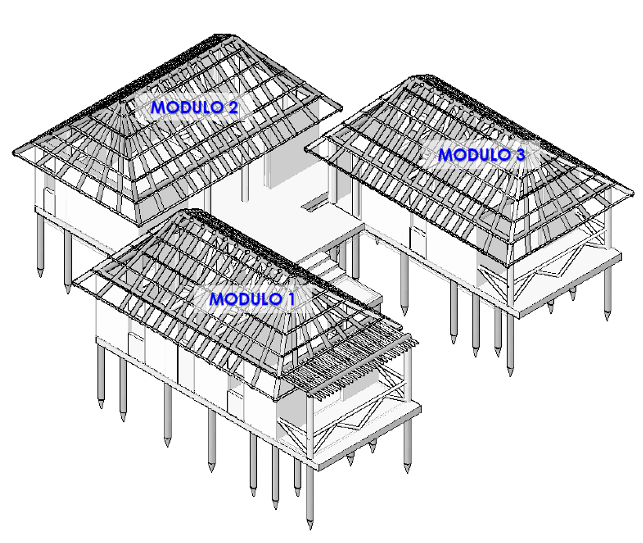
\includegraphics{texto-img/texto-img002.png}  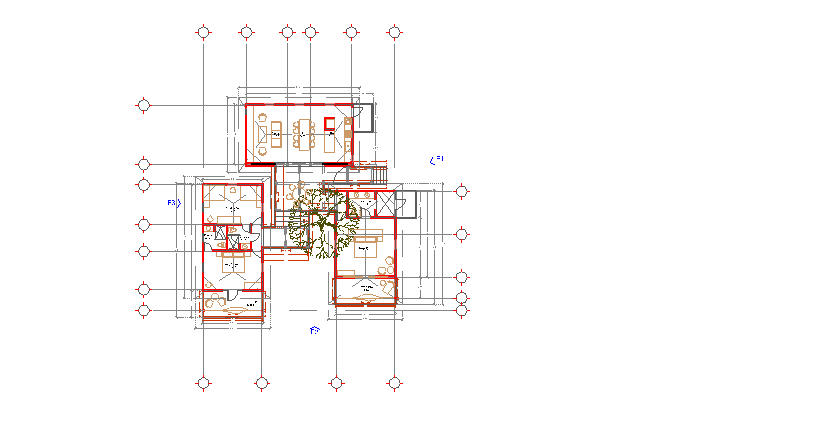
\includegraphics{texto-img/texto-img003.png} 


\bigskip

Figura \stepcounter{Figura}{\theFigura}. Agrupación de módulos (izquierda) y la planta arquitectónica (derecha) de una unidad tipo “Palafito”.


\bigskip


\bigskip

Las actividades para la construcción de un palafito inician con las acciones preliminares comunes en cualquier obra, las cuales son la colocación de señalización preventiva y restrictiva así como barreras físicas para impedir el impacto visual y generar un ingreso controlado al sitio de la obra. También se colocarán los contenedores para residuos sólidos urbanos en el sitio previamente autorizado. Dichas actividades preliminares incluyen además: la preparación del sitio, apertura de brecha, limpieza de elementos extraños y retiro de basura, trazo y ubicación de áreas de aprovechamiento y desplante de edificaciones con equipo topográfico de precisión satelital. 


\bigskip

El desmonte, se realizará únicamente en aquellas áreas que sea necesario, por ejemplo donde la vegetación rebase la altura del palafito; según el caso, se realizará el desenraice y remoción o poda de ejemplares arbóreos o arbustivos empleando medios manuales (palas, motosierras, podadoras, etc.) y mecánicos donde sea necesario. En caso de requerir medios mecánicos se empleará la mini cargadora Bobcat misma que se desplazará únicamente dentro del área a intervenir y que por su tamaño compacto (3.30 m de longitud por 1.60 m de ancho) resulta útil para evitar generar impactos adicionales fuera del límite aprovechable.


\bigskip

Dado al sistema constructivo a emplear de forma elevado sobre terreno natural, el despalme no es requerido en todo el elemento, sino únicamente en los sitios donde se desplantarán los rollizos (ver más adelante su definición). Únicamente se procederá a acarrear el material resultante del desmonte, auxiliándose de medios manuales (carretillas) así como la maquinaria antes descrita hasta las brechas existentes en el sitio, las cuales debido a que ya se encuentran previamente impactadas, permiten el acceso de maquinaria de mayor tamaño para recibir el material de desmonte y transportarlo hasta el sitio autorizado para su alojamiento.


\bigskip

Los dos insumos más representativos en este sistema constructivo son la madera y la palma. Ambos insumos provendrán de sitios debidamente certificados por la SEMARNAT para su venta y tratamiento, donde serán sometidos a procedimientos de preservación en talleres especializados. Dichos insumos serán almacenados y protegidos apropiadamente, contra cambios en su contenido de humedad y daño mecánico, de tal manera que siempre satisfaga los requerimientos del proyecto. Antes de la construcción, la madera se secará a un contenido de humedad apropiado (18\%) y tan parecido como sea práctico al contenido de humedad en equilibrio promedio de la región. Derivado del tratamiento previo por empresas especializadas, fuera del PDV, la madera estará exenta de infestación activa de agentes biológicos como hongos e insectos así como posteriores efectos del intemperismo. Se cuidará que la madera esté debidamente almacenada y protegida durante toda la vida útil de la estructura. 


\bigskip

Para efectos de la construcción de palafitos, los trabajos para el corte, armado y detallado de las piezas se ejecutará en el taller de carpintería del proyecto en las obras provisionales temporales, fuera del área de dunas, para luego trasladar dichas piezas ya cortadas en la medida requerida al sitio de obra, donde se habilitarán para su instalación y se harán pequeños ajustes que se requieran.


\bigskip

En las actividades de transporte y montaje, se cuidará que el ensamblaje de estructuras se lleve a cabo en tal forma que no se produzcan esfuerzos excesivos en la madera no considerados en el diseño. Los miembros torcidos o rajados más allá de los límites tolerados en la norma NMX-C-224-ONNCCE, serán reemplazados.


\bigskip

Además se hará uso de las brechas existentes y estacionamientos que se destinarán al proyecto, a fin de que el suministro de insumos así como la circulación de vehículos y personal se efectúe por estos caminos, reduciendo así los impactos a otras coberturas. El perímetro del área aprovechable será delimitado con malla sombra para evitar la circulación fuera de esta superficie.


\bigskip

Los rollizos hincados son piezas estructurales fundamentales en el sistema constructivo del Palafito, son los elementos de anclaje y soporte del mismo, el cual da estabilidad, firmeza y permanencia en el lugar del hincado. Para su transporte se empleará un vehículo tipo Torton de cama baja, el cual tiene capacidad para transportar, en un solo viaje, la madera necesaria para construir hasta dos módulos. Dicho vehículo podrá circular únicamente en las brechas existentes (ya impactadas) y en las áreas que se destinarán a vialidades del proyecto, empleando los estacionamientos del proyecto para efectuar cualquier maniobra de carga o descarga y retorno. Se empleará de forma auxiliar un vehículo dotado de brazo grúa para transportar las piezas a aquellas áreas de cobertura vegetal sensible y evitar el rodamiento de vehículos pesados en dichas coberturas. De igual forma todas las piezas que conforman el sistema de palafitos se transportarán ya cortadas y listas para el habilitado de acuerdo a las dimensiones requeridas por el plano de despiece.


\bigskip

 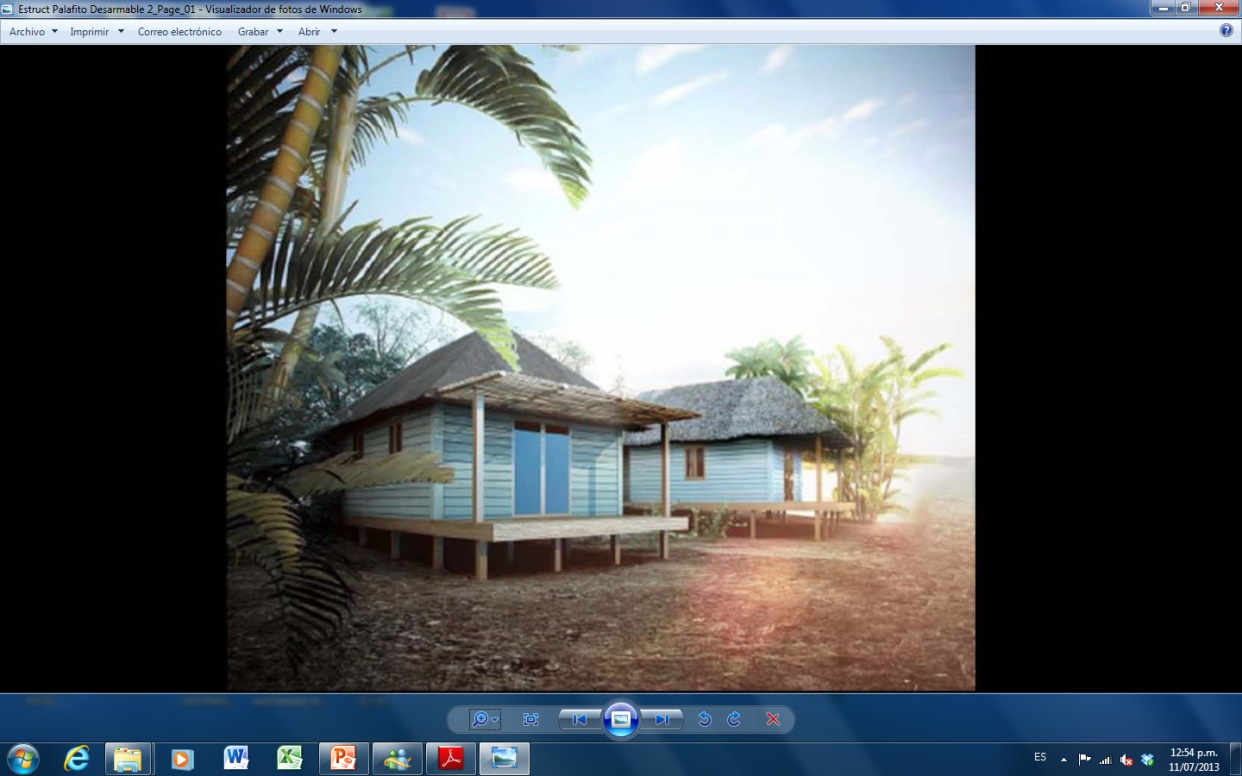
\includegraphics{texto-img/texto-img004.jpg} 


\bigskip

Figura \stepcounter{Figura}{\theFigura}. Apariencia exterior de las edificaciones tipo palafitos.


\bigskip


\bigskip

El sistema constructivo, como ya se mencionó anteriormente, establece que la cimentación de los palafitos estará conformada por rollizos de madera Chiché de nomenclatura (CM) con una sección redonda de 30 cm desplantados aproximadamente a 0.60 m sobre terreno natural que serán apuntalados a una profundidad aproximada de 80 cm o bien lo que determine el estudio de mecánica de suelos específico. Esto se efectuará de tal manera que garantice su integridad estructural y se alcance la integración deseada con el suelo.


\bigskip

La cimentación será de bajo impacto, pues únicamente se desplantará el área donde se excavará para hincar los rollizos que soportarán los palafitos. Al tratarse de una plataforma sostenida únicamente por rollizos de madera los cuales van hincados al terreno natural, se evita la extracción de arena de las playas y dunas costeras (y su consecuente erosión y alteración de la dinámica costera) provocada por cimentaciones convencionales que requieren grandes volúmenes de excavación. 


\bigskip

Previo al hincado, se ubicarán los sitios de perforación de acuerdo al proyecto. El área circundante al punto de hincado de cada rollizo, es decir, en un radio aproximado de 2.50 m del rollizo, será preparada para recibir el marco hidráulico apuntalador así como la rejilla donde se asentarán los sacos de arena. Dicha preparación consiste únicamente en despejar el área de cualquier objeto extraño y, de ser necesario, nivelar manualmente cualquier amontonamiento de arena que impida o dificulte la estabilidad del equipo y la maniobra del hincado.


\bigskip

El marco apuntalador para realizar las labores de hincado de rollizos se carga fácilmente con ayuda de dos personas. El hincado de cada rollizo se lleva alrededor de 4 horas, mientras que el armado de la estructura del palafito se tomará poco más de 2 semanas empleando una cuadrilla de 4 personas, considerando que las piezas ya estarán perforadas y habilitadas de forma que únicamente se proceda a su instalación.


\bigskip

El proceso de preparación para el hincado incluye las siguientes actividades:


\bigskip

\begin{enumerate}
\item Se arma el marco principal con las columnas C-1 y la viga T-1.
\item Se colocan las rejillas y se unen entre sí sobre cada una de las placas base de las columnas.
\item Sobre las rejillas se colocan los sacos de arena (suministrados previamente y rellenos con arena proveniente de bancos de material autorizados) distribuidos como se indica en el detalle correspondiente.
\item Para efectos del apuntalado se realizará una perforación previa a manera de guiar el rollizo durante el hincado y evitar que se produzca un pandeo o se introduzca de forma inclinada, además esto facilita el acceso a los estratos resistentes y evita movimientos excesivos en la masa de suelo adyacente. La perforación será de 80 cm de profundidad por 40 cm de diámetro. Para esto sólo se requiere una excavación mínima de un diámetro menor a 30 cm, la cual se realizará por medios manuales; en ningún caso se extraerá arena de la zona, el material resultante de la perforación es reintegrado nuevamente al suelo.
\item Se coloca el poste en la perforación previa y se fijan las guías T-2 con tornillos en las bases correspondientes de la columna C-1.
\item Se coloca el capuchón en la parte superior del poste y se acomoda el gato hidráulico en reposo en la parte central entre el capuchón y el riel.
\item Se repite el primer procedimiento para después colocar la base auxiliar 02 y 03.
\item El hincado de cada poste finalizará una vez que los sacos de arena se comiencen a levantar, este será el indicador que se obtuvo la capacidad de carga requerida. Los sacos de arena funcionarán como un mecanismo de contrapeso y serán reutilizables en todos los procesos de hincado de rollizos.
\end{enumerate}
 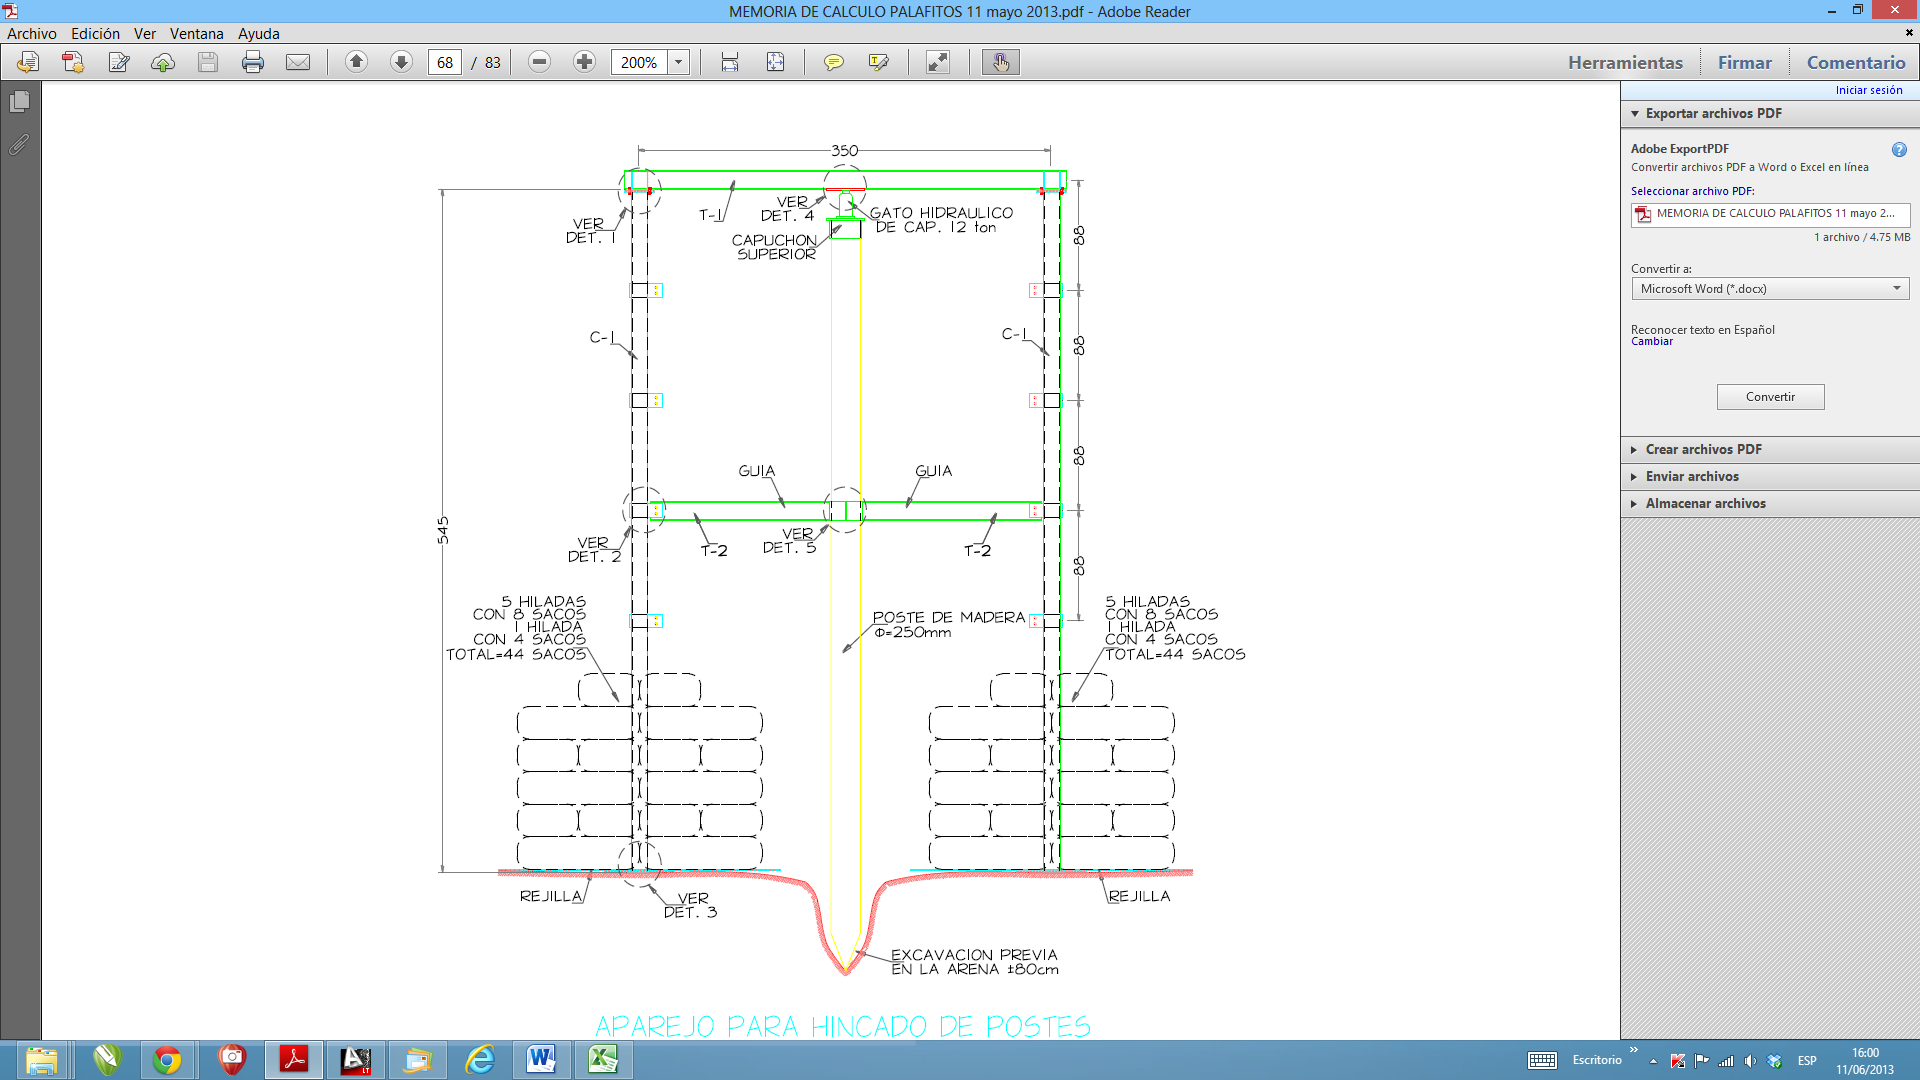
\includegraphics{texto-img/texto-img005.png} 

Figura \stepcounter{Figura}{\theFigura}. Aparejo para hincado de rollizos.


\bigskip


\bigskip

Los rollizos serán hincados a presión por un aparejo lastrado con sacos rellenos de arena proveniente de bancos de material autorizados, en ningún caso se empleará ni retirará arena del sitio. Estos sacos o costales de arena serán de una dimensión aproximada de 102 cm x 51 cm x 25 cm y pesarán en promedio 60 kg. Se requerirán 44 costales por columna para ejercer una presión de 2,640 kg. Se colocarán 5 hiladas de costales en forma cuatrapeada en cada una de las rejillas en el desplante de la columna.


\bigskip

 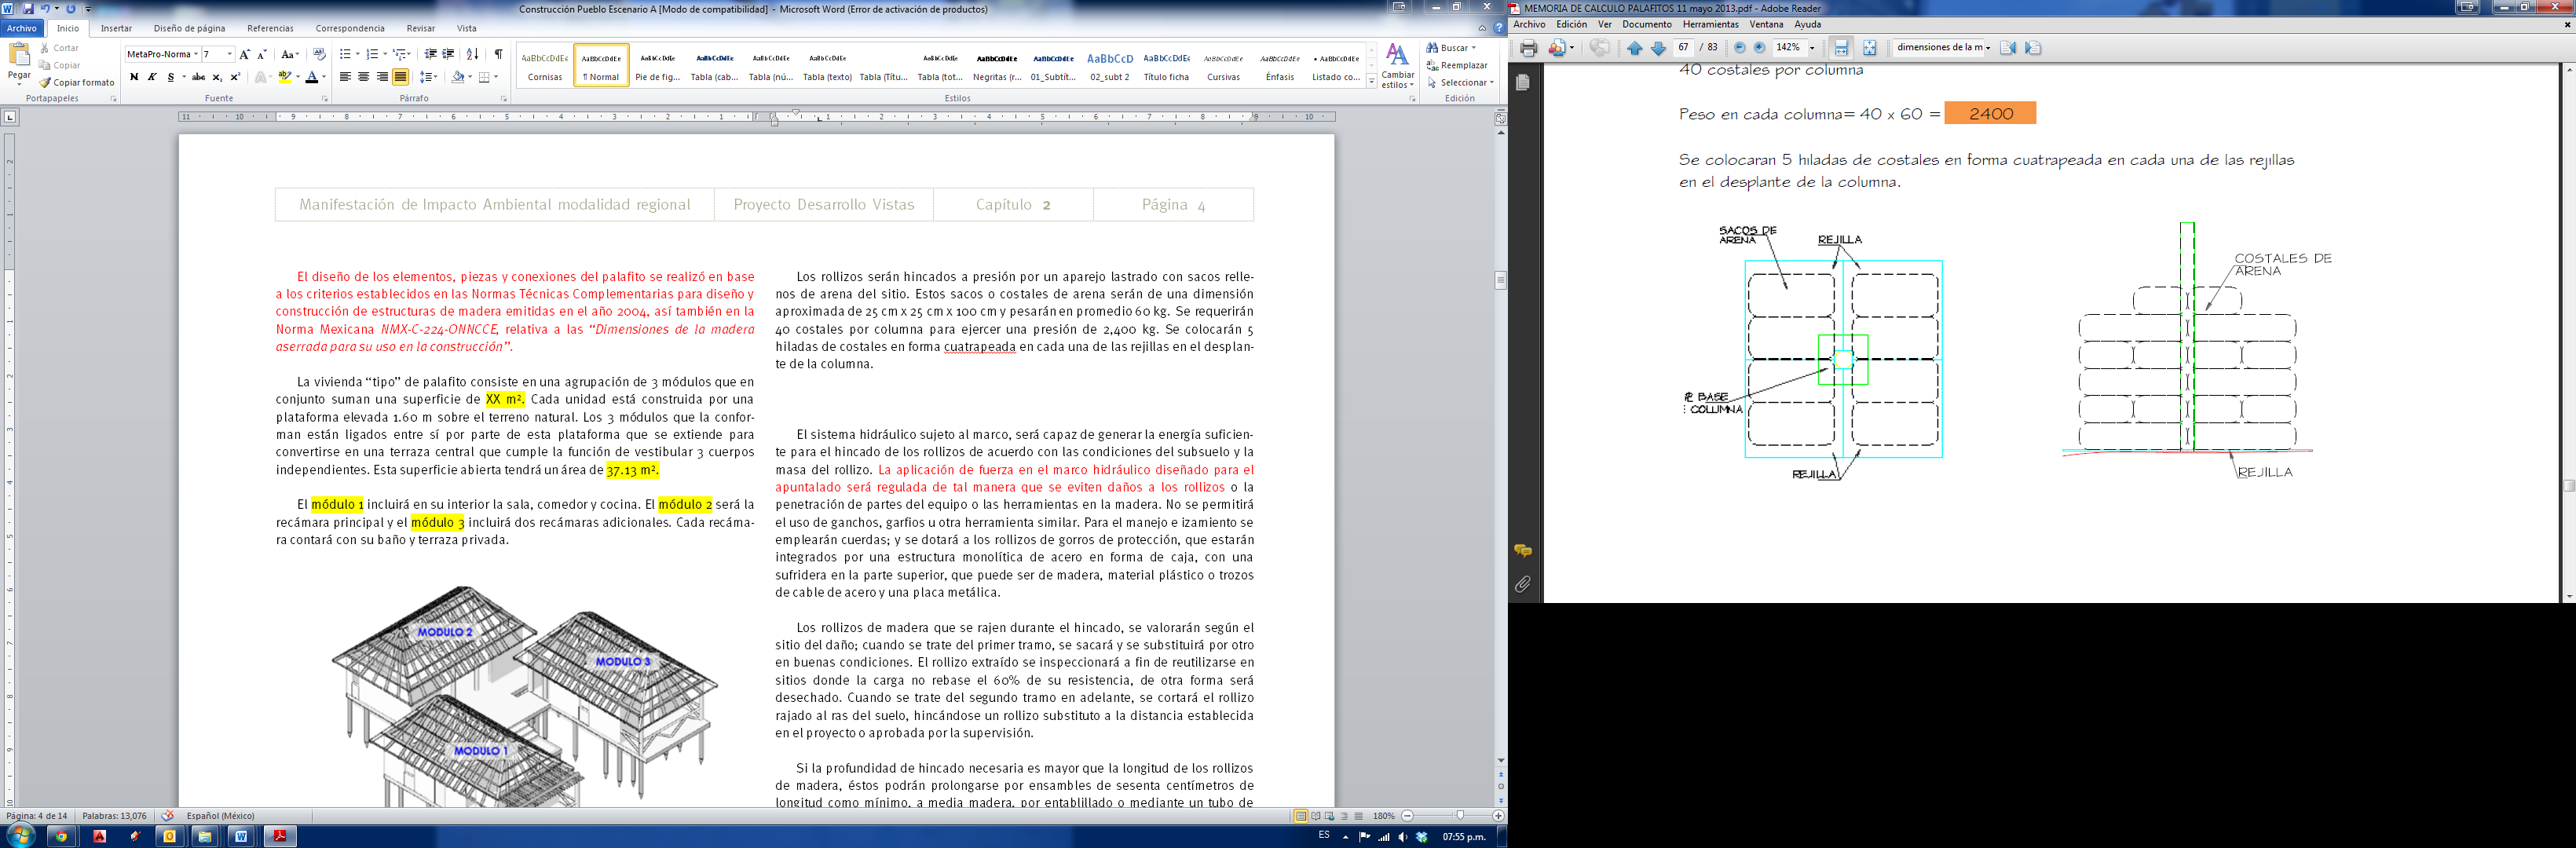
\includegraphics{texto-img/texto-img006.png} 

Figura \stepcounter{Figura}{\theFigura}. Disposición de los sacos de arena para el hincado.


\bigskip


\bigskip

El sistema hidráulico sujeto al marco, será capaz de generar la energía suficiente para el hincado de los rollizos de acuerdo con las condiciones del subsuelo y la masa del rollizo. La aplicación de fuerza en el marco hidráulico diseñado para el apuntalado será regulada de tal manera que se eviten daños a los rollizos o la penetración de partes del equipo o las herramientas en la madera. No se permitirá el uso de ganchos, garfios u otra herramienta similar. Para el manejo e izamiento se emplearán cuerdas; y se dotará a los rollizos de gorros de protección, que estarán integrados por una estructura monolítica de acero en forma de caja, con una sufridera en la parte superior, que será de madera, material plástico o trozos de cable de acero y una placa metálica.


\bigskip

El hincado de cada poste se finalizará una vez que las bases de los sacos de arena se comiencen a levantar, esta será la indicación de que se obtuvo la capacidad de carga requerida, por lo que la profundidad de los postes será variable. Cuando las columnas del marco comiencen a dejar de hacer contacto con la superficie, indica que se ha alcanzado la presión necesaria para el hincado.


\bigskip

Los rollizos de madera que se rajen durante el hincado, se valorarán según el sitio del daño; cuando se trate del primer tramo, se sacará y se substituirá por otro en buenas condiciones. El rollizo extraído se inspeccionará a fin de reutilizarse en sitios donde la carga no rebase el 60\% de su resistencia, de otra forma será desechado. Cuando se trate del segundo tramo en adelante, se cortará el rollizo rajado al ras del suelo, hincándose un rollizo substituto a la distancia establecida en el proyecto o aprobada por la supervisión. 


\bigskip

Si la profundidad de hincado necesaria es mayor que la longitud de los rollizos de madera, éstos se prolongarán por ensambles de 60 cm de longitud como mínimo, a media madera, por entablillado o mediante un tubo de acero en el que se introduzcan los extremos de las dos piezas por unir. Se llevará a cabo una bitácora semanal del hincado de rollizos y se entregará a una empresa con la especialidad de mecánica de suelos para la revaloración de datos que arrojen cambios en la profundidad de hincado. Con el propósito de evitar la erosión de la arena el mayor tiempo posible, se colocarán sacos de arena alrededor del poste una vez terminado el hincado.


\bigskip

Los extremos superiores de los rollizos hincados serán descabezados; se cortarán a escuadra y al nivel establecido en el proyecto, hasta ajustarlas al plano de la parte inferior de la estructura que se apoye en ellos. Una vez que los rollizos de madera hayan sido cortados al nivel establecido, a las cabezas se les hará un reforzamiento con cuerda, similar al usado en amarres de palapa.


\bigskip

Se programará el hincado con rollizos de forma que después de alcanzar la profundidad requerida por proyecto, sobresalga del terreno natural una columna de 60 cm abajo del nivel de lo que será el piso terminado. Se preparará el ensamble por entablillado o mediante encofrado de un tubo de acero en el que se introduzcan los extremos de las dos piezas por unir, de esta forma la estructura desde el entrepiso podrá llegar fabricada en tableros al lugar de su instalación. En el caso de elegir el encofrado por tubo de acero, una vez realizado el corte del rollizo hincado se preparará para recibir la espiga con doble punta y así los extremos se acoplan a presión al dilatar la madera; en caso de optar por el llamado entablillado, se harán las perforaciones para colocar las planchas metálicas.


\bigskip

La estructura de Palafito es de Clase “B”, debido a que su mayor dimensión ya sea horizontal o vertical, varía entre 20 y 50 m; correspondiéndole un periodo de retorno de 50 años (Ver documento anexo “Memoria de cálculo estructural para la construcción de palafito de tres cuerpos, en polígono poblado pescadores del desarrollo inmobiliario nombrado Proyecto Chalacatepec en el municipio de Tomatlán, Jalisco” en el apartado 7 “Análisis Dinámico de Viento” y el documento anexo Normas y especificaciones para estudios, proyectos, construcción e instalaciones; Volumen 4: Seguridad Estructural; Tomo III Diseño por Viento del Instituto Nacional de la Infraestructura Física Educativa donde se citan las especificaciones a observar para el diseño de estructuras por viento).

 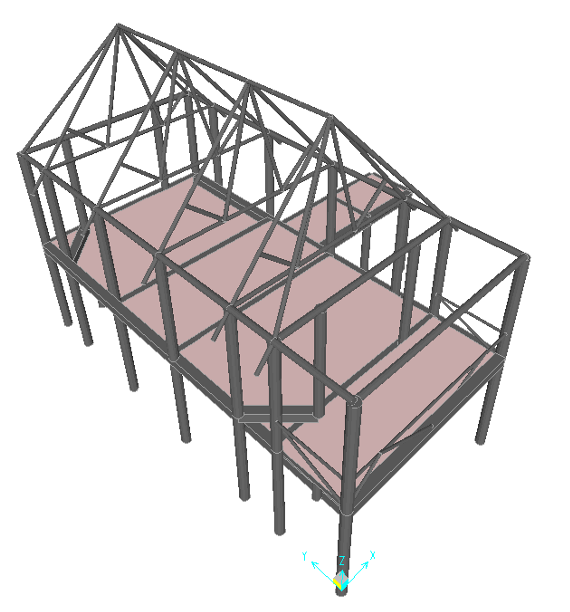
\includegraphics{texto-img/texto-img007.png}  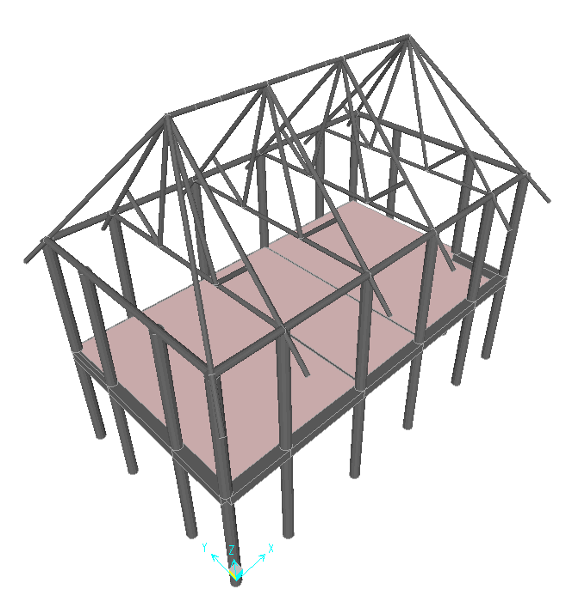
\includegraphics{texto-img/texto-img008.png}  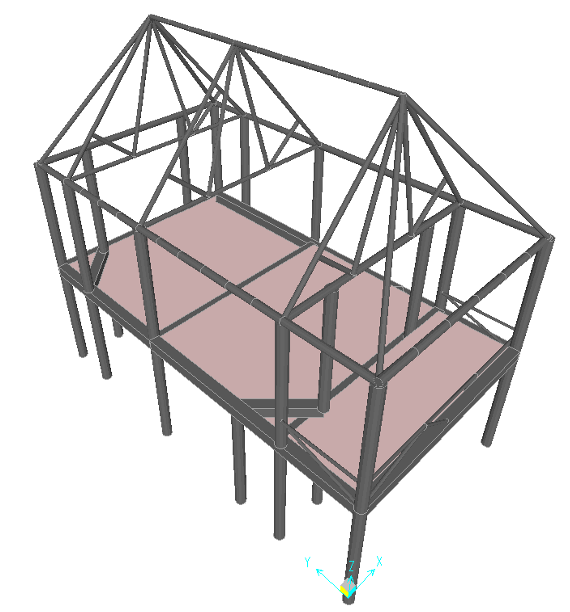
\includegraphics{texto-img/texto-img009.png} 

Figura \stepcounter{Figura}{\theFigura}. Isométrico de la estructura de cada uno de los módulos.


\bigskip


\bigskip

La estructura de la edificación se conforma de un entrepiso de madera y una cubierta de tipo palapa apoyada en armaduras y ramadas. El sistema de pisos y techos está conformado por elementos estructurales de madera denominados vigas secundarias (T-P) apoyadas en vigas madrinas principales interiores (T-D’) y exteriores (T-D) para conformar un diagrama rígido. El piso será de madera y se instalará a una altura de 0.60 m para mantener el movimiento natural de la arena, que la vegetación pueda seguir desarrollándose y la fauna pueda tener libre paso. 


\bigskip

 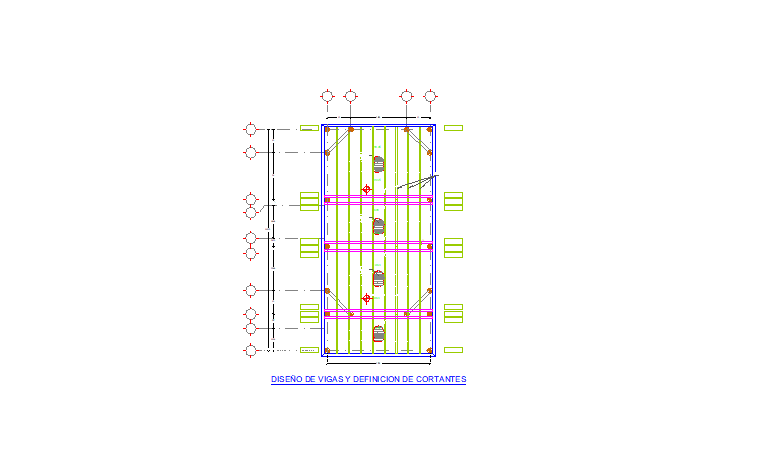
\includegraphics{texto-img/texto-img010.png} 

Figura \stepcounter{Figura}{\theFigura}. Distribución de vigas y definición de cortantes.


\bigskip


\bigskip

Estará constituido a base de duela de 1ª de 1”x3”x8 pies sujeta directamente a la estructura de vigas de madera. Dado el diseño de los palafitos, el entrepiso más pequeño pesa 4,963 kg. Se propone construir en 8 secciones o tableros sobre las vigas madrinas que forman parte del entrepiso (1,804 kg), quedando en secciones que no superen los 450 kg, donde sus conexiones se diseñaron con tornillos especificados en la norma NMX-H-47.


\bigskip

Bajo el piso de madera se instalarán de forma suspendida con ayuda de abrazaderas, los conductos que distribuirán al interior de la vivienda, las diferentes redes hidráulicas, sanitarias, eléctricas, de telecomunicaciones y de gas. 


\bigskip

De forma específica el suministro de gas será por medio de recipientes portátiles o cilindros de 30 Kg ubicados al exterior de cada unidad palafito. Por su forma, peso y dimensiones se pueden mover fácilmente para su reposición los cuales serán reemplazados cada mes en camionetas o vehículos repartidores de 3 t.


\bigskip

La localización de estos recipientes será en aquellos sitios con las mejores condiciones de ventilación natural y con un espacio suficiente (no menor a 9 m²) para realizar las maniobras de conexión e instalación sin riesgos. Sobre el cilindro y de forma accesible se tendrá la válvula de paso con operación manual, la cual regulará el cierre o apertura del suministro. Además, el cilindro contará con una válvula de seguridad, cuya función es proteger a los recipientes en caso de que presenten sobrepresiones interiores peligrosas. Estas válvulas están diseñadas de forma que no permiten que estén en contacto con el gas líquido y sólo con la zona de vapor, por lo que será obligatorio mantener los recipientes portátiles siempre en posición vertical.


\bigskip

A partir de este punto se instalará una línea de conducción empleando de tuberías y accesorios de cobre que quedarán fijadas de forma superficial en la edificación, esto para acceder fácilmente para una reparación en caso de fuga. Dichas tuberías conducirán hasta las llaves de paso o corte manual que se instalarán de forma individual en cada aparato o equipo que requiera el suministro, o bien para regular ciertas secciones de la instalación.


\bigskip

Las tuberías podrán ser de cobre rígido y flexible en aquellos puntos donde se requiera, generalmente a proximidad del cilindro o de los equipos que realizan el consumo; y se fijarán a los muros de forma estable y alineada, para lo cual se utilizarán dispositivos de fijación como abrazaderas o clips. 


\bigskip

Para el manejo e instalación de la tubería de cobre, se cortará el tubo de la dimensión que se requiera empleando un cortador especial y se lijarán los extremos para eliminar cualquier imperfección o rebaba. Se identificarán las piezas y conexiones a utilizar. Posteriormente se empleará una avellanador para formar la campana del tubo e insertar la pieza roscada que permitirá unir dos tubos mediante coples.


\bigskip

El trazo de las tuberías será el más corto y rectilíneo posible hasta los distintos puntos de utilización y en función de que la tubería no se exponga a choques. Los tramos de tubería que deban colocarse de forma subterránea (a una profundidad mínima de 60 cm) o que transcurran a través de muros, serán provistos de una funda de acero o insertos en una tubería tipo conduit. Sin embargo, la tubería de gas se mantendrá superficial en todo momento, permitiendo únicamente su empotramiento en muros como medio de transición entre las diversas áreas de la edificación y en distancias cortas. Las uniones de los tubos serán roscadas y acopladas por medio de herrajes y conectores. 


\bigskip

Bajo el piso, se tendrá cuidado en la distribución de las tuberías que irán suspendidas, en función de que exista un mínimo de 20 cm de separación constante entre las tuberías de gas y conductores eléctricos o fluidos de alta presión.


\bigskip

El cálculo estructural del palafito se basa en normas publicadas por el gobierno federal mexicano a través del INIFED. Una de las reglas del procedimiento constructivo para las conexiones es que los agujeros para alojar los pernos en la madera deberán taladrarse de manera que su diámetro no exceda al del perno en más de 2 mm, ni sea menor que el diámetro del perno más un milímetro. Se cumplirá con el espaciamiento entre pernos, sea entre pernos de una hilera y el espaciamiento entre hileras de pernos, así como se vigilará se cumpla la distancia a los extremos y a los bordes.


\bigskip


\bigskip

 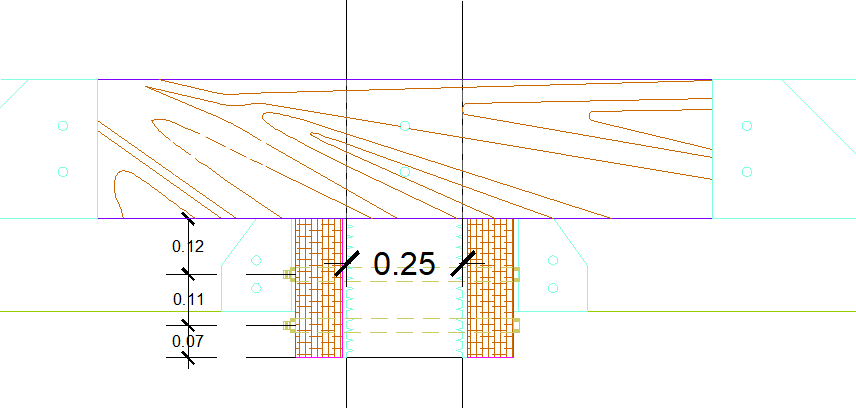
\includegraphics{texto-img/texto-img011.png} 

Figura \stepcounter{Figura}{\theFigura}. Conexión de rollizos verticales.


\bigskip


\bigskip

En las vigas madrinas exteriores deberán revisarse los defectos propios de la madera por elaboración, cuidados en el almacenamiento, protección en pie de obra y desinstalación, debido a que estos factores repercuten de manera directa en la resistencia o desempeño de las piezas en servicio. En lo que respecta a los mecanismos de conexión, se sustituyó en gran parte la tornillería auto-roscante por placas dentadas o pernos; en ambos casos (placas o pernos), el análisis de su utilización consideró las características físicas de la madera Chiché y si las cargas ahora aplicadas son paralelas o perpendiculares a las fibras.


\bigskip

 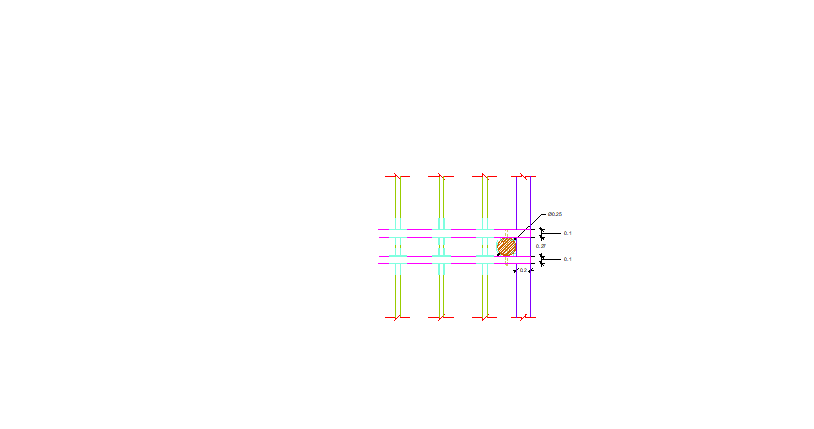
\includegraphics{texto-img/texto-img012.png} 

Figura \stepcounter{Figura}{\theFigura}. Conexión de rollizos a viga madrina.


\bigskip


\bigskip

El acomodo de las vigas permite usar placas dentadas y pernos, que se emplearán como sistema de unión entre los rollizos y las vigas para lograr una cara plana en lugar de circular, logrando que parte de la transferencia de carga se efectúe por medio de los dientes formados en las placas. Se tendrá especial cuidado en que la placa no se deforme durante su instalación, que los dientes sean perpendiculares a la superficie de la madera, que la madera bajo las placas no tenga defectos y que el grosor mínimo de los miembros unidos sea el doble de la penetración de los dientes.

Existen diferentes proveedores de conexiones metálicas para madera, razón por la cual para evitar que surjan problemas durante y después de la edificación de los palafitos, se demostrará experimentalmente que las uniones son adecuadas, mediante pruebas de prototipos de nodos donde se utilicen dichas uniones. Se realizarán los ajustes necesarios de las dimensiones de la pieza, del calibre, del fy del acero, incluso del galvanizado, de igual forma se harán las anotaciones pertinentes en la bitácora.


\bigskip

La utilización de los pernos consisten en piezas de bajo carbono especificadas en la norma NMX-H-47 “Tornillos con cabeza hexagonal” basadas en las Normas Técnicas Complementarias para Madera; mientras que en el caso de placas dentadas, las mismas Normas Técnicas señalan que las placas serán de lámina galvanizada con las propiedades mínimas indicadas en la norma NMX-B-009, con la denominación de “Láminas de acero al carbón galvanizadas por el proceso de inmersión en caliente“. Los prototipos antes mencionados deben cumplir con lo señalado en el inciso 6.4.2 sub-inciso a) de dichas normas, antes de su fabricación y montaje.


\bigskip

 \includegraphics{texto-img/texto-img013.png}   \includegraphics{texto-img/texto-img014.png} 

Figura \stepcounter{Figura}{\theFigura}. Tipos de conexiones para madera empleadas.


\bigskip


\bigskip

Los muros serán elementos rígidos conformados por forros exteriores de madera Chiche (Aspidosperma megalocarpon) de 2”x4”x8 pies, tendrán una altura total de 2.40 m. El despiece de las secciones de muros estarán regidos por el proyecto y por el peso, el primero lo determina el espacio entre los rollizos y entre los claros de puertas y en segundo punto se buscará que no rebase los 300 kg, el cual es diferente a los tableros de entrepiso que pueden llegar a pesar 450 kg, esto debido a que dichos muros contarán con vanos en el sitio donde se ubiquen las ventanas y puertas y su colocación será vertical. Los muros se clasificarán en exteriores, divisorios interiores secos y divisorios interiores húmedos, los cuales, corresponden a los que se colocarán en baños.


\bigskip

Los muros exteriores estarán conformados por tableros con el acabado en la cara exterior según el proyecto ejecutivo; tendrán un forro a base de tablas de 25 cm colocadas horizontalmente y sujetas a un bastidor de barrotes de madera colocados verticalmente a cada 61 cm o menos según el claro, por ejemplo: si la longitud es de 3.25 m, se inicia con un barrote colocado verticalmente a 0.61 m, el segundo a 1.22 m, el tercero a 1.83 m, el cuarto a 2.44 m, el quinto a 3.05 m y el sexto a 3.25 m. Donde se localicen ventanas de una hoja los barrotes serán de 0.04x0.10x1.20 m y en donde se encuentre una ventana de dos hojas los barrotes medirán 0.04x0.10x0.90.


\bigskip

 \includegraphics{texto-img/texto-img015.png} 


\bigskip

Figura \stepcounter{Figura}{\theFigura}. Disposición de muros exteriores.


\bigskip


\bigskip

Los muros divisorios interiores en su cara hacia el interior llevarán un forro de panel de madera, que en lo subsecuente se llamará panel OSB (Oriented Strand Board~=~tablero de virutas orientadas) de 1.22x2.44x0.19 m. Es un tablero que se fabrica con virutas de madera que son cortadas tangencialmente a partir de los troncos previamente descortezados, las virutas resultantes son posteriormente prensadas sometiéndolas a presiones y temperaturas determinadas. Las virutas que conforman el panel OSB van dispuestas en capas perfectamente diferenciadas y orientadas: las capas exteriores son orientadas generalmente en dirección longitudinal mientras que las virutas de las capas internas son orientadas en dirección perpendicular a la longitud del panel.


\bigskip

De acuerdo a normas que estandarizan desde su fabricación hasta su utilización, la norma EN 300 define cuatro tipos de panel OSB en función de sus propiedades mecánicas y resistencia a condiciones húmedas. Se emplearán dimensiones específicas para los muros de baños; por su parte los del palafito en general se utilizará un panel de 2,400mm x 1,200mm x 12mm que pesa aproximadamente 20 kg.


\bigskip

Los tableros se fijarán conforme a los siguientes pasos:


\bigskip

\begin{enumerate}
\item Se atornillarán orientando el lado largo de los tableros paralelos (en sentido vertical) a los postes del bastidor, o bien perpendiculares a ellos (en sentido horizontal).
\item Todas las juntas verticales coincidirán con los ejes de los postes.
\item La fijación de los tableros será con tornillos tipo S a no más de 30.5 cm de separación, comenzando del centro de los tableros hacia las orillas.
\item Para la colocación horizontal se fijarán primero los tableros superiores para no apoyarlos sobre los inferiores. Se alternarán las juntas entre tableros en cualquiera de las dos aplicaciones por ambos lados del muro. 
\end{enumerate}

\bigskip

Es conocido que el acabado de las hojas de virutas orientadas es irregular y que al ser fijadas con tornillo auto-roscante se generan juntas y pequeñas deformaciones. Asimismo, en el lugar donde se construirán los palafitos la humedad relativa supera el 80\%, razón por la que será forrado con sistema de malla y pasta plástica que será preparada en el taller donde se armen los paneles y aplicada con llana metálica. Para instalarlo se seguirán los siguientes pasos:


\bigskip

\begin{enumerate}
\item Una vez atornillado el panel OSB al bastidor, se aplicará con llana una primera capa de pasta plástica en todas las juntas e hilera de tornillos, se dejará secar 2 horas.
\item Seguido se aplicará una segunda capa de pasta plástica con espesor aproximado 2.5 mm, enseguida se colocará la malla de refuerzo en toda la superficie y se dejará secar otras 2 horas.
\item Por último se aplicará una tercera capa de pasta, buscando con la llana metálica dejar el acabado semi pulido.
\end{enumerate}

\bigskip

Para los muros interiores de baños y cocina se utilizará OSB/3 - Tableros estructurales para utilización en ambiente húmedo. Estos muros, además de seguir el mismo procedimiento que para los muros divisorios normales, se considerará la instalación de la tubería de agua potable y drenaje y se fijará con abrazaderas con neopreno de baja densidad o poliestireno de alta densidad entre los bastidores y la tubería, para evitar el golpe de ariete y daño durante la vida útil. En la fabricación de muros con el sistema antes descrito, se considera el uso de tornillos tipo pija, mismos que serán de acero de bajo carbono, especificados en la norma NMX-H-23 “Tornillos de acero para madera”.

 \includegraphics{texto-img/texto-img016.png} 


\bigskip

Figura \stepcounter{Figura}{\theFigura}. Detalle de muros interiores en baños y áreas húmedas.


\bigskip

Las zonas expuestas directamente al agua como regaderas, llevarán además del panel, un recubrimiento con malla de polipropileno, pasta tipo base Coat y un recubrimiento adicional de vitrificado que consiste en azulejo de barro esmaltado o cerámica cocida al horno en piezas de 0.20 m por lado. Tal como se observa en el detalle siguiente:

 \includegraphics{texto-img/texto-img017.png} 


\bigskip

Figura \stepcounter{Figura}{\theFigura}. Detalle de recubrimiento en áreas expuestas al agua.


\bigskip

Para alojar las pijas se cuidará satisfacer los siguientes aspectos: 


\bigskip

\begin{enumerate}
\item El taladro guía para la caña tendrá el mismo diámetro que la caña y su profundidad será igual a la longitud del tramo liso de ésta.
\item El taladro guía para el tramo con rosca tendrá un diámetro entre 40 a 70 por ciento del diámetro de la caña que corresponde para maderas del grupo III, que son Latifoliadas y que fue elegido en la memoria de cálculo considerando los resultados del laboratorio realizados por la Universidad Autónoma de Guadalajara, para probetas enviadas para ensayo de la madera Chiché.
\end{enumerate}

\bigskip

Los espaciamientos y las distancias a los bordes y los extremos para uniones con pijas se vigilarán que estén cerca del centro del barrote del bastidor, sea este vertical u horizontal, considerando que habrá junta de paneles OSB en un mismo barrote, al igual que la duela en el entrepiso.


\bigskip

 \includegraphics{texto-img/texto-img018.png} 

Figura \stepcounter{Figura}{\theFigura}. Apariencia del muro interior armado sobre bastidores.


\bigskip

En lo que refiere a la cubierta, consistirá en un techo inclinado a dos o más aguas, conformado por armaduras de madera que se apoyarán directamente en la estructura de corona conformada por los rollizos hincados (ahora columnas en la edificación). La palapa se calculó con armaduras que trabajan bajando su carga directamente a las columnas de rollizos, estos elementos se unirán con conectores de sujeción y tornillería.

 \includegraphics{texto-img/texto-img019.png} 

Figura \stepcounter{Figura}{\theFigura}. Conexión estructural de muro y cubierta.


\bigskip

La cubierta de la edificación tendrá una cumbrera de 3 m al centro en el sentido longitudinal, dando un total al centro de 5.40 m, estará formado por armaduras de madera que soportarán los bastidores redondos de madera, que conformarán las superficies inclinadas. Se recurrirá a la palma utilizada en la región de la Costa Norte de Jalisco, la denominada Palma Real (Sabal~Mexicana) la cual se encuentra disponible en la región y se suministrará a través de proveedores debidamente registrados ante la SEMARNAT, utilizando para el bastidor o estructura de fijación madera Chiche o Guayabillo. La palapa tejida a base de hojas de “Palma Real” tendrá un espesor de 10 a 14 cm y se llevará a cabo principalmente por artesanos de la región. Para la elaboración de un metro cuadrado de palapa se requiere un promedio de 100 hojas de palma de un metro de largo por 0.5 cm de grosor, dichas hojas serán previamente tratadas en talleres especializados fuera del proyecto.


\bigskip

 \includegraphics{texto-img/texto-img020.jpg} 

Figura \stepcounter{Figura}{\theFigura}. Corte esquemático “tipo” del sistema constructivo palafitos.


\bigskip

 \includegraphics{texto-img/texto-img021.png} 

Figura \stepcounter{Figura}{\theFigura}. Componentes de la cubierta de palapa.


\bigskip

Las puertas y ventanas incluyendo marco, jamba y otras molduras necesarias para su correcto funcionamiento, serán fabricadas con madera de Parota o huanacaxtle (Enterolobium cyclocarpum). La selección en la madera a emplear reside en que otro tipo de maderas requieren gran cantidad de químicos para resistir la termita o polilla y deben ser recubiertas con tintas para dar un color uniforme, en el caso de la Parota o huanacaxtle no es necesario. El proyecto contará con tres tipos de puertas: abatibles de exterior, de interior y puertas para baños. 


\bigskip

Las puertas estarán conformadas por un bastidor que recibirá las planchas de madera (llamadas tableros), en una hendidura central. El bastidor estará formado por dos largueros (elementos verticales), y travesaños (elementos horizontales), que fijan los tableros. En el larguero opuesto es donde se colocan las bisagras y batientes. El cabezal es el travesaño superior y el peinazo el travesaño de mayor ancho, generalmente ubicado en la parte inferior y en algunos casos, a la altura de la cerradura. El bastidor tiene un espesor de 45 mm, el ancho de largueros y travesaños es de 90 mm y el ancho del peinazo es de 190 mm.


\bigskip

 \includegraphics{texto-img/texto-img022.jpg} 

Figura \stepcounter{Figura}{\theFigura}. Componentes de las puertas del proyecto.


\bigskip

Los elementos del bastidor estarán unidos a través de un ensamble de caja y espiga, a menudo con una clavija de madera como refuerzo. No se utilizarán adhesivos, para permitir los cambios volumétricos por las variaciones de la humedad ambiente. Todos los herrajes y tornillería serán galvanizados dadas las condiciones climáticas del sitio. Los tableros estarán formados por la unión de varias tablas para obtener el ancho deseado, el que conviene reforzar con tarugos. Sus bordes, de menor espesor y caras inclinadas, se insertan en la ranura de los largueros y travesaños, sin colocar adhesivos por la razón antes mencionada.

 \includegraphics{texto-img/texto-img023.jpg}  \includegraphics{texto-img/texto-img024.jpg} 


\bigskip

Figura \stepcounter{Figura}{\theFigura}. Elementos y uniones del bastidor.


\bigskip

Previo a la instalación, es importante revisar que las dimensiones cumplan con el proyecto y no rebasen las tolerancias antes señaladas y preparar en el lugar de la obra donde se almacenarán temporalmente con las condiciones óptimas para su estiba, asegurándose además de mantenerlas en posición vertical sobre una superficie seca, nivelada y en su embalaje original, conservando los elementos transitorios que se usaron en el transporte, protegidas del clima, polvo y daños. 


\bigskip

Una adecuada colocación de las puertas asegurará una mayor durabilidad, facilidad de operación y mantenimiento. Se verificará que se cuente con las herramientas apropiadas para su instalación y para controlar la geometría de vanos, puertas y ventanas. Para ello se verificará la horizontalidad del dintel y la verticalidad de las jambas, con ayuda del nivel carpintero y plomada mecánica.

 \includegraphics{texto-img/texto-img025.jpg}   \includegraphics{texto-img/texto-img026.jpg} 

Figura \stepcounter{Figura}{\theFigura}. Verificación del dintel y jambas con nivel.


\bigskip

Para la colocación de cuñas entre el marco y las jambas del tabique, es importante que el marco quede bien ajustado en el vano, evitando espacios excesivos que permitan el paso del aire de un lado a otro, una holgura no mayor de 5 mm, que será rellenada desde ambos paramentos. Para cubrir la junta entre puerta o ventana y jamba, es necesaria la colocación de una moldura. Dependiendo de cómo cierren las puertas en los baños y en las recamaras, se elijará el tipo de bisagra y un pasador removible para su desinstalación en caso de ser requerida.


\bigskip

En las ventanas es importante considerar que, en la zona donde se proyectan los palafitos, la presión de viento en los meses de junio a octubre presenta velocidades altas, razón por la que se construirán con travesaños y largueros, lo que divide el claro y aporta mayor resistencia. Cada bastidor o conjunto de elementos que conforman una hoja de ventana está constituido por largueros (elementos verticales), travesaños (elementos horizontales intermedios), cabezal y peinazo (elemento horizontal inferior). El larguero es el elemento vertical que recibe las bisagras mientras que el elemento vertical opuesto se denomina batiente.


\bigskip

El marco correspondiente a la estructura que rodea la ventana y que se fija al vano, estará constituido por dos piezas verticales denominadas jambas, y dos horizontales llamadas cabios, la superior denominada dintel y la inferior peana. El marco se dividirá por piezas verticales intermedias, llamadas montantes o por una pieza horizontal que se conoce como imposta. Las diferentes piezas o perfiles de madera que conformarán las ventanas tendrán un espesor de 45 mm, salvo en el caso de las ventanas de los baños, las cuales tendrán un espesor de 32 mm.


\bigskip

 \includegraphics{texto-img/texto-img027.jpg}  \includegraphics{texto-img/texto-img028.jpg}  \includegraphics{texto-img/texto-img029.png}  \includegraphics{texto-img/texto-img030.png} \newline


Figura \stepcounter{Figura}{\theFigura}. Características y composición de las ventanas.


\bigskip

Se colocarán barandales de madera en las terrazas de los módulos uno y tres. De acuerdo a la variedad de claros a proteger, los tramos de barandal se subdividieron en módulos, quedando con dimensiones entre 0.79 y 0.82 cm de longitud. Se analizó una figura geométrica que permita dar seguridad para un nivel 80-5 (personas de 80 años o más y niños de 5 años), y como segundo punto el que pueda ser desarmable. Siguiendo la temática ecológica propuesta, el barandal se construirá de madera y sus diferentes tramos tendrán dimensiones a construir en taller y posteriormente ser trasladados como una sola pieza al sitio de la obra.


\bigskip

 \includegraphics{texto-img/texto-img031.png} 

Figura \stepcounter{Figura}{\theFigura}. Alzado de un tramo del barandal existente en el módulo 1.


\bigskip

 \includegraphics{texto-img/texto-img032.jpg} 

Figura \stepcounter{Figura}{\theFigura}. Acabados exteriores de un palafito.


\bigskip


\bigskip

Sistema constructivo de edificaciones convencionales


\bigskip

En esta sección se describe el proceso constructivo de aquellas edificaciones que se construirán empleando sistemas convencionales, por lo que las actividades de preparación son las comunes en cualquier obra, mismas que consisten en la colocación de señalización preventiva y restrictiva así como barreras físicas para impedir el impacto visual y generar un ingreso controlado al sitio de la obra; se colocarán tambos de 200 L rotulados, como contenedores para residuos en el sitio previamente autorizado. Posteriormente, se realizará la limpieza del sitio, trazo del terreno con equipo topográfico de precisión satelital, apertura de brecha y desmonte, incluyendo desenraice y remoción o poda de ejemplares arbóreos dentro del área a construir. Posteriormente se realizará el despalme con maquinaria de manera exclusiva en las áreas de aprovechamiento (a excepción de las áreas que serán destinadas para jardines) y por último el acarreo por medios mecánicos de material resultante hasta el sitio autorizado para su alojamiento en las obras temporales del componente. Se nivelará el terreno en aquellas áreas que, por proyecto, sea necesario.


\bigskip

El sistema constructivo de este componente incluirá cimentación y elementos estructurales (dalas medianeras, y de cerramiento, castillos, columnas) a base de concreto armado. Se realizarán las excavaciones necesarias para la cimentación de acuerdo a lo indicado en los planos del proyecto y se procederá a la colocación de una plantilla de concreto pobre de f’c~=~100 kg/cm² con un espesor de 5 cm con la finalidad de colocar el acero de refuerzo de la zapata y evitar que este se contamine cuando se realice el vaciado del concreto protegiéndolo del contacto con el terreno natural. Como parte integral de esta etapa del proceso estará el habilitado y armado de acero de refuerzo en elementos de cimentación y estructurales con un límite de fluencia Fy~=~4200 kg/cm2 actividad realizada de acuerdo a las Normas Mexicanas NMX-B-294-1986 y NMX-C-407-ONNCCE-2001, en diferentes diámetros de acuerdo a lo indicado en el proyecto estructural. Esta actividad se realizará en los talleres establecidos para tal fin en las obras provisionales temporales, a manera de evitar contaminación en el sitio de trabajo por los desperdicios y generar menos presión al sitio de obra.


\bigskip

Se procederá al habilitado de cimbra para la cimentación y elementos estructurales de concreto. Se utilizará madera de segunda y/o contrachapada (tipo triplay), aglomerados, polines y largueros. En algunos casos se utilizarán elementos metálicos. Toda la cimbra cumplirá con las especificaciones técnicas y diseño señaladas en el proyecto. El habilitado y preparación de cimbra se realizará en talleres ubicados en las obras provisionales temporales. Una vez que se tengan los elementos de acuerdo a los requerimientos del proyecto se trasladarán a donde se requieran; el empleo de la cimbra se hará de forma adecuada a fin de potencializar su vida útil para su reutilización. El 100\% de la cimbra de madera está sujeta a reutilizarse siempre y cuando se manipule correctamente. Las piezas que conforman la cimbra de contacto, (la que está directamente en contacto con el concreto: tablas, tableros de triplay) tienen una vida útil de cinco a siete usos. Por su parte la cimbra complementaria, también llamada obra falsa (madrinas, cargadores, puntales, arrastres y otros) tiene una vida útil de ocho a 10 usos (ver Medidas de prevención, mitigación y compensación de impactos ambientales: generales).

Para el colado de elementos estructurales se empleará concreto premezclado bombeable suministrado por empresas de la región; en los casos donde se requiera de concreto elaborado en el sitio se procederá a construir una plataforma de madera tipo artesa, para evitar contaminar el concreto y de la misma forma evitar la contaminación del área de trabajo. La resistencia del concreto (f`c) variará de acuerdo a lo especificado en el proyecto. Previo al vaciado se humedecerá la cimbra para evitar que esta absorba la humedad del concreto. El vibrado de concreto se realizará por medios mecánicos; dicha actividad es importante para evitar burbujas de aire y la segregación de agregados. Posteriormente se procederá al curado del mismo mediante el riego, para evitar la pérdida rápida de humedad, empleando aguas claras, o mediante la aplicación de alguna membrana de curado, al menos durante un periodo de tres días. 


\bigskip

El descimbrado de los elementos estructurales, se realizará hasta que el concreto alcance la resistencia necesaria para que soporte su peso propio y las cargas de construcción o según la duración que especifique el proyecto de acuerdo al concreto empleado. Una vez terminadas las actividades de descimbrado, la madera que aún pueda ser reutilizada será almacenada en el taller de obra temporal del componente.


\bigskip

La edificación se conformará por muros de block (tabique o tabicón), confinados por castillos y cadenas de concreto armado; habrá también muros de piedra braza de la región. La elaboración del mortero será mediante una revolvedora mecánica y se almacenará en una artesa de madera para evitar que se contamine el área de trabajo y el mortero propio, los agregados serán suministrados de bancos de material en la región debidamente autorizados por la autoridad competente. 


\bigskip

Los acabados en muros serán aplanados de cemento cal y arena en diferente terminado (bruñido, manoseado, apalillado, esponja, etc.) y con pintura vinílica; muros recubiertos con materiales pétreos, mosaicos de pasta o cerámica en diferentes colores lisos o con dibujos estampados; se emplearán muros bajos de piedra acomodada sin mortero tipo tecorral o muros de mampostería de piedra.


\bigskip

El sistema de losas y cubiertas será variado, incluirá cubiertas planas compuestas de ladrillo de medio pliego y una capa de compresión de concreto, apoyados sobre vigas de madera; cubiertas aligeradas con casetón de poliestireno apoyadas sobre vigas de madera y ladrillo de medio pliego, cubiertas a base de losa llena de concreto reforzado con acero, cubiertas inclinadas con estructura de madera y teja, cubiertas de vigueta y bovedilla; techumbres a dos aguas soportadas por armaduras de acero o madera y cubiertas con teja de barro recocido. Para el desalojo del agua pluvial, las cubiertas planas serán dotadas de bajantes que conducirán el agua de lluvia a andadores y jardines para su reabsorción al suelo. Más allá de la cubierta, los muros se extenderán para integrarse a un pretil de 1.80 m de alto, rematado por una moldura de concreto que funciona como dala de coronación. 


\bigskip

Se usarán varios sistemas de impermeabilización, esto de acuerdo a los elementos a impermeabilizar. En todo momento se verificará que los productos a emplear sean adquiridos en puntos de distribución certificados. En los tanques y cisternas de almacenamiento, se utilizará impermeabilizante integral en el concreto, con colado monolítico o con el menor número de juntas. Los muros de contención en contacto con la humedad del subsuelo, se impermeabilizarán por la cara interior. En las losas de concreto, se hará de acuerdo al sistema indicado en el proyecto.


\bigskip

Los acabados en pisos de terrazas, andadores, circulaciones interiores y exteriores podrán ser mosaicos de pasta en colores sólidos o estampados, pisos de concreto acabado pulido, arcilla prensada o compactada, piedra laja o cantera, empedrados de piedra bola asentadas sobre arena, etc. Debido a que existe una gran variedad de opciones a emplear, para efectos del cálculo de materiales y mano de obra, a fin de tener una imagen homogénea se tomaron en cuenta aquellos acabados empleados en el componente Hacienda-Xala, en el que predominan mosaicos de pasta, empedrados, piedra laja y cantera.


\bigskip

La carpintería de piezas como pérgolas, puertas, closets, ventanas y demás elementos señalados en el proyecto a ejecutarse de este material, será de madera certificada proveniente de establecimientos debidamente autorizados (a excepción de la cimbra, la cual será de madera de segunda obtenida en los establecimientos autorizados en el área de Tomatlán). Los herrajes serán comerciales de uso común con tratamiento galvanizado para ampliar su vida útil dada las características climatológicas del sitio del proyecto; la vidriería será translúcida o con ornamentación según proyecto; los muebles y accesorios de baños tendrán dispositivos ahorradores de agua. Los materiales y procedimientos de suministro y colocación cumplirán con las especificaciones generales del proyecto ejecutivo así como la normatividad vigente.


\bigskip

Para finalizar el proceso de construcción se realizarán las pruebas de funcionamiento, en esta etapa se verifica que todo haya sido realizado de acuerdo a las Normas Oficiales Mexicanas y Normas Técnicas vigentes así como a las especificaciones generales del proyecto ejecutivo. Se probará el correcto funcionamiento de todas y cada una de las partes que la integran, como son: instalación eléctrica, instalación sanitaria, hidráulica, instalaciones especiales, aire acondicionado, voz y datos, tableros, controles, accesorios, por último el arranque de los equipos.


\bigskip

Para el suministro de gas en edificaciones convencionales se instalarán tanques de almacenamiento estacionario de 120 L, 300 L o 500 L (o la capacidad que el uso que vaya a darse a la edificación requiera) los cuales se ubicarán generalmente en la azotea o en áreas al exterior de la edificación que cuenten con buen flujo de ventilación natural. Se instalará una toma en un sitio accesible al frente de la vivienda, misma que contará con una válvula de servicio con maneral fijo, indicador de máximo llenado y tubo de profundidad con deflector y medidor de nivel de líquido. En dicha toma se realizará el suministro por medio de carros pipa. 

 \includegraphics{texto-img/texto-img033.png} 

Figura \stepcounter{Figura}{\theFigura}. Diagrama básico de instalación de un tanque estacionario. \newline
Tomado de: Enríquez Harper, El ABC de las instalaciones de gas, hidráulicas y sanitarias, página 42 capítulo 1.


\bigskip


\bigskip

A partir de este punto se instalará una línea de conducción empleando de tuberías y accesorios de cobre que quedarán fijadas de forma superficial en la edificación, esto para acceder fácilmente para una reparación en caso de fuga. Dichas tuberías conducirán hasta las llaves de paso o corte manual que se instalarán de forma individual en cada aparato o equipo que requiera el suministro, o bien para regular ciertas secciones de la instalación.


\bigskip

Las tuberías podrán ser de cobre rígido y flexible en aquellos puntos donde se requiera, generalmente a proximidad de los equipos que realizarán el consumo; y se fijarán a los muros de forma estable y alineada, para lo cual se utilizarán dispositivos de fijación como abrazaderas o clips. 


\bigskip

Para el manejo e instalación de la tubería de cobre, se cortará el tubo de la dimensión que se requiera empleando un cortador especial y se lijarán los extremos para eliminar cualquier imperfección o rebaba. Se identificarán las piezas y conexiones a utilizar. Posteriormente se empleará una avellanador para formar la campana del tubo e insertar la pieza roscada que permitirá unir dos tubos mediante coples.


\bigskip

El trazo de las tuberías será el más corto y rectilíneo posible hasta los distintos puntos de utilización y en función de que la tubería no se exponga a choques. Los tramos de tubería que deban colocarse de forma subterránea (a una profundidad mínima de 60 cm) o que transcurran a través de muros, serán provistos de una funda de acero o insertos en una tubería tipo conduit. Sin embargo, la tubería de gas se mantendrá superficial en todo momento, permitiendo únicamente su empotramiento en muros como medio de transición entre las diversas áreas de la edificación y en distancias cortas. Las uniones de los tubos serán roscadas y acopladas por medio de herrajes y conectores. 


\bigskip


\bigskip

Sistema constructivo de vialidades secundarias y estacionamientos de empedrado en arena


\bigskip

Se optó por emplear una superficie de rodamiento rústica a base de empedrado asentado en arena, misma que armoniza con la imagen urbana que se pretende dar del contexto. Lo anterior corresponde a una vialidad de bajo a mediano impacto ya que permite la correcta absorción del agua pluvial al subsuelo, no alterando los flujos hídricos naturales de los que depende la integridad funcional de las Áreas Prioritarias para la Conservación. 


\bigskip

La construcción de este tipo de vialidades conlleva las actividades preliminares comunes a cualquier obra: señalizaciones, colocación de elementos de protección, trazo de superficie aprovechable con equipo topográfico de precisión, limpieza, apertura de brecha y desmonte y finalmente despalme de capa vegetal. El material de despalme obtenido en el proceso se reservará en un sitio específico en las obras temporales y será confinado con sacos de arena u otro material para protegerlo de los efectos erosivos eólicos e hídricos para su posterior uso en actividades de jardinería.


\bigskip

Se realizará la excavación por medios mecánicos hasta una profundidad de 0.40 m para efectos del mejoramiento del suelo de desplante. Una vez alcanzado el nivel establecido para el proyecto, se nivelará y compactará la superficie y se realizará la aportación de material de banco o del sitio para la conformación de la capa subrasante. Nuevamente se nivelará y compactará por medios mecánicos y posteriormente se colocará la capa de base, empleando material hidráulico controlado de 20 cm de espesor.


\bigskip

Las vialidades de empedrado serán a base de piedra bola de río de canto rodado con un espesor promedio de 15 cm. Previo a su colocación se escarificarán hasta 2 cm de espesor de la capa de arena para facilitar el hincado de la piedra, esto empleando picos y rastrillos. Una vez disgregada la capa de arena, la piedra será colocada a mano, empleando un martillo o mazo de 2 kg, que servirá para el hincado. Se colocarán las piedras maestras o cordones maestros con la piedra de mayor tamaño en los ejes, bordes o límites de carriles. Adicionalmente deben colocarse maestras longitudinales intermedias entre el eje y el borde del camino. La distancia entre maestras no será mayor a 1.50 metros. 


\bigskip

Conformadas las maestras, se completará el rodamiento con la colocación de piedra de menor tamaño (8 a 12 cm), de tal manera que se logre un confinamiento adecuado entre las piedras, procurando disminuir al máximo los espacios intersticiales que se formen. Inmediatamente se esparcirá material de relleno en los espacios entre las piedras para aumentar la adherencia entre éstas y disminuir la filtración excesiva de agua pluvial que pueda ocasionar un deslizamiento. Este material será de las mismas características de la capa de base y cubrirá por completo las piedras. A este proceso se lo conoce como emporado. Una vez concluido, se compactará la piedra mediante el paso sin vibración de un rodillo liso de 4 a 8 toneladas, iniciando el trabajo en los costados y desplazándose hacia el centro. 


\bigskip

En función de los sitios donde se construyan cunetas, la vialidad tendrá pendientes del 2\% en el sentido de la ubicación de la cuneta o en ambos sentidos a partir del eje de la misma para encauzar el agua pluvial hacia el terreno natural. 


\bigskip

La construcción de cunetas inicia con el trazo de los límites de la misma de acuerdo a la sección específica del proyecto, la cual es de 0.60 m de ancho. El proceso continúa con la excavación de 0.40 m de profundidad para la conformación de la base de la cuneta. El material producto de la excavación será retirado para confinarse en las obras temporales del componente.


\bigskip

 \includegraphics{texto-img/texto-img034.png} 

Figura \stepcounter{Figura}{\theFigura}. Detalle constructivo de cuneta.


\bigskip

Se humedecerá la superficie de base de la cuneta, se conformarán taludes según la pendiente especificada en el proyecto ejecutivo, empleando material producto de la excavación; se afinará y compactará mediante pisón metálico de mano de al menos 15 kg, garantizando una compactación del 90\% como mínimo. Seguido, se colocarán la cimbra metálica, dejando una junta fría de 1 cm de espesor a intervalos no mayores a tres metros.


\bigskip

Se colocará la malla electrosoldada o el acero de refuerzo que especifique el proyecto, y se verterá el concreto, comenzando por el extremo inferior de la cuneta y avanzando en el sentido ascendente de la misma, verificando en todo momento que su espesor sea de 10 cm. A la superficie de concreto se le aplicará una membrana de curado para concreto sin diluir. La cimbra permanecerá en su sitio al menos durante un lapso de 48 horas.


\bigskip

Para concluir el proceso, se perfilará la superficie de la cuneta y se corregirán las irregularidades superficiales mediante la aplicación de mortero. Una vez curado el concreto y retirada la cimbra, se limpiarán las juntas y de colocará un sellador. El material de escombro será recolectado y enviado al sitio previamente asignado en las obras temporales del componente. Se realizará una limpieza general y los contenedores de basura serán retirados.

Las áreas de estacionamiento de vehículos se construirán empleando el sistema constructivo descrito anteriormente. Dichas superficies contarán con pendientes en función de conducir el agua pluvial hacia trampas de grasas donde puedan captarse eventuales derrames de combustible o cualquier tipo de grasa que pueda contaminar de manera irreversible el agua. Se procurará que a partir del estacionamiento, únicamente circulen vehículos de menor peso relacionados con la vigilancia, la protección civil, investigación científica y conservación biológica, en cuyo caso se utilizarán vehículos tipo carritos de golf, cuatrimotos o similares.


\bigskip

Concluida la construcción de la superficie de rodamiento, se colocarán los indicadores de alineamiento, las cuales consistirán en señales bajas utilizadas para delinear la orilla del carril de circulación e indicar cambios en el alineamiento horizontal, estrechamiento de la corona y los extremos de muros de puentes y pasos pluviales. Estos dispositivos de señalamiento se conocen comúnmente como “fantasmas” y consisten en postes prefabricados a base de concreto, de color blanco y de un metro de altura, dotados de una franja reflejante en la parte superior, colocado de manera que refleje hacia el flujo de circulación de los vehículos y a la altura de la luz que incide de los faros.


\bigskip

Las actividades de obra concluirán cuando la superficie se encuentre lista para la circulación, y se remplacen los elementos de protección y señalización provisionales por los elementos de información y señalización vial de acuerdo a las normas de SCT; así como la recolección y acarreo de residuos hasta el sitio autorizado así como las labores de limpieza del sitio.


\bigskip

Dado el procedimiento constructivo a emplear, la generación de residuos de manejo especial (RME) consistirá en la merma de residuos de obras asociadas a la vialidad, como hilo, pedaceria de madera proveniente de la señalización, restos de piedra, empaques y embalajes varios, etc.; así como los residuos provenientes de los aglutinantes empleados.


\bigskip


\bigskip

Sistema constructivo de albercas convencionales


\bigskip

La construcción de albercas se realizará con el sistema convencional hecha en obra que consiste en una fosa integrada por muros y losa de concreto armado con acero. Su ejecución implica la preparación del sitio mediante la colocación de la señalización preventiva y restrictiva necesaria. Se ubicarán los contenedores de residuos y se realizará la limpieza y desmonte del terreno, seguida del trazo de la fosa de las dimensiones que indique el proyecto, empleando para ello un equipo topográfico de precisión. 


\bigskip

Se realizará la excavación de la fosa por medios mecánicos en cualquier material hasta la profundidad de acuerdo al proyecto, efectuando el afine de la misma y la compactación del suelo al 90\% de su prueba proctor estándar una vez alcanzado el nivel de desplante. El material resultante de la excavación será acarreado en camión hasta el sitio autorizado para su emplazamiento en las obras temporales.


\bigskip

Posteriormente se forjarán firmes y muros de concreto premezclado con una resistencia mínima de f’c~=~250 kg/cm² armado con acero de refuerzo fy~=~4,200 kg/cm² y con otras características adicionales que especifique el desarrollador. Para tal efecto se empleará cimbra de madera proveniente de establecimientos autorizados o cimbra metálica. Los muros tendrán una altura estándar de 1.50 m.


\bigskip

Las escaleras de ingreso serán parte del diseño establecido por el desarrollador, pudiendo ser prefabricadas o parte integral de la alberca, forjadas con block de jalcreto asentado con mortero cemento- arena, acabados según proyecto. El diseño de los acabados de recubrimiento se establecerá en el proyecto ejecutivo, para tal efecto se emplearán materiales vidriados tales como el mosaico veneciano en diversos tamaños y colores; pudiendo sustituirse por otros acabados según especifique el proyecto. 


\bigskip

Finalmente, se construirá a proximidad un cuarto de máquinas empleando sistemas constructivos convencionales antes descritos; se instalará el equipo electromecánico necesario para garantizar el correcto funcionamiento de la alberca, empleando sistemas de limpieza y desinfección que a su vez permitan el ahorro de agua.


\bigskip


\bigskip

Sistema constructivo de cuerpo de agua artificial


\bigskip

Para complementar las obras de paisajismo se habilitará un cuerpo de agua artificial con una profundidad aproximada de 1.20 m. Dicho cuerpo de agua se ubicará en la parte Este del Pueblo, cercano al consultorio, estacionamiento y plaza de espectáculos públicos. Como se mencionó al inicio del documento, además de tener una función ornamental, este elemento fungirá como receptor del agua tratada proveniente de la PTAR del componente, en aquellas temporadas de lluvia donde eventualmente se pueda presentar un excedente en el volumen de agua tratada disponible, ya que la demanda de agua para riego se podrá ver disminuida. 


\bigskip

Para la construcción del cuerpo de agua artificial se colocará la señalización preventiva y restrictiva y se realizará la excavación de la fosa por medios mecánicos. Posteriormente se conformarán los taludes con material producto de la excavación, se nivelarán y compactarán al 90\% prueba proctor y se recubrirán con una capa de 20 cm de espesor de arena de granulometría controlada para la conformación de la base de desplante del cuerpo de agua. El material resultante de la excavación será acarreado en camión hasta el sitio autorizado para su emplazamiento temporal.


\bigskip

Se habilitarán tubos de respiración de 4” de diámetro recubiertos con malla geotextil tipo pavitex 200 o similar. Se colocará el refuerzo a base de liner de triple capa conformado por dos capas exteriores de Geomembrana de caucho sintético tipo EPDM 1.02 mm o similar y una capa central de geotextil 200 gr/m² tipo pavitex 200 o similar. Se realizará el recubrimiento de taludes con material pétreo en capas de 5 cm de espesor sin juntear ni asentar; se colocará el resto del equipo de recirculación del agua, iluminación y accesorios.


\bigskip


\bigskip

Sistema constructivo de áreas verdes ornamentales


\bigskip

Estos espacios se reforestarán conforme a la naturaleza de su ecosistema, empleando en todos los estratos vegetación endémica y vegetación adaptada a la región que no represente riesgo de desplazamiento de las especies locales. En seguimiento a lo anterior, en el componente Pueblo se empleará la vegetación primaria existente, aprovechando áreas de vegetación impactada o de menor calidad ambiental y generando una gran área de vegetación al concentrar el palmar existente hacia el noroeste del predio. Además, este macizo vegetal evitará la emisión de luz artificial o resplandor proveniente de las edificaciones hacia la playa de anidación de tortugas. Además, dicha intervención se ubicará alrededor de las edificaciones del Pueblo, esto con el fin de crear un confinamiento del mismo por medio de una barrera de palmeras y evitar así su crecimiento descontrolado.


\bigskip

Se prevé el trasplante de 491 palmeras (Cocos nucifera) existentes en el polígono del PDV, de las cuales 295 serán palmas chicas con una altura de 2 a 4 m y las 196 palmas restantes serán medianas; contarán con una altura aproximada de 4 a 6 m. 


\bigskip

Los trabajos preliminares consistirán en verificar que previo a su traslado, cada palmera cuente con la marca de su orientación magnética y el ángulo de inclinación con respecto a la horizontal, las cuales se respetarán durante todo el proceso de trasplante. Esto se marcará con pintura que no dañe la palmera.


\bigskip

 \includegraphics{texto-img/texto-img035.jpg} 

Figura \stepcounter{Figura}{\theFigura}. Palmar existente.


\bigskip

El envasado consistirá en humedecer el suelo correspondiente al área de goteo de la palmera para facilitar la remoción de tierra y formación del cepellón. Es muy importante señalar que, en época de lluvias, se evaluará en el sitio y en el momento de los trabajos, la consistencia del suelo y cantidad de agua que exista en la tierra del área de goteo. El cepellón se protegerá con costales de yute u otro material fácilmente degradable que garantice la forma del cepellón, atándolo con materiales de la misma característica que podrán dejarse enterrados al ser plantada la palmera. Por ningún motivo se utilizarán plásticos. 


\bigskip

 \includegraphics{texto-img/texto-img036.jpg} 

Figura \stepcounter{Figura}{\theFigura}. Tratamiento al cepellón de palmera.


\bigskip

Para el traslado de las especies se hará uso de las brechas existentes o aquellas áreas que serán destinadas a las vialidades del componente, a fin de que el suministro de palmeras, la circulación de vehículos y personal se efectúe por estos caminos, reduciendo así los impactos a otras coberturas. El transporte de las palmeras se realizará en un camión de plataforma o Torton de cama baja. Se empleará de forma auxiliar un vehículo dotado de brazo grúa para transportar las piezas a aquellas áreas de cobertura vegetal sensible y reducir aún más el rodamiento de vehículos en dichas coberturas.


\bigskip

En la maniobra de reubicación, se protegerá el tronco en la zona de izaje con yute u otro material que evite el degüello o lastime la corteza de la palmera. En la colocación se cuidará que el cepellón quede centrado en la cepa y se le dará a la palmera la inclinación y orientación original, hasta que el nivel superior del cepellón quede a nivel de terreno natural.


\bigskip


\bigskip

 \includegraphics{texto-img/texto-img037.jpg}   \includegraphics{texto-img/texto-img038.jpg} 

Figura \stepcounter{Figura}{\theFigura}. Transporte y colocación de palmeras (para efectos de ilustrar el procedimiento).


\bigskip


\bigskip

En el sitio del proyecto, se realizará la ubicación y el trazo de los sitios donde se plantarán los ejemplares empleando para ello equipo topográfico de precisión satelital. Se limpiará y desmontará el área de plantación y se procederá a realizar la excavación de la cepa con la holgura suficiente que permita maniobrar al interior de la misma para la colocación adecuada del cepellón; las dimensiones de la cepa serán de 2.40 m por lado y 0.90 m de profundidad. Posteriormente, se realizará el acarreo de tierra vegetal proveniente de las actividades de despalme, previamente separada y almacenada en las obras temporales del componente para el mejoramiento de la tierra donde se plantará la palmera. 


\bigskip

Se rellenará la cepa con tierra vegetal hasta el nivel del terreno natural circundante y se compactará el suelo empleando equipo manual para el auto sustento de la palmera y finalmente se dejará un pequeño borde con el diámetro del área de goteo para la retención del agua de riego o lluvia. Terminados los trabajos, se retirarán los residuos que pudieran generarse así como el material producto de la excavación para confinarlo en las obras temporales del componente para posteriormente emplearlo en otros sitios que se requiera.


\bigskip


\bigskip

Sistema constructivo de terrazas, patios y explanadas


\bigskip

A fin de minimizar el impacto a la conectividad de la vegetación natural y a las áreas de movilización de fauna silvestre, las vialidades de circulación peatonal o de vehículos ligeros consistirán en suelo natural sin ningún tipo de recubrimiento, su principal función será la intercomunicación de todas las áreas y de aquellas que por su cercanía a la playa fungen únicamente como accesos al mar y donde la circulación será únicamente peatonal. 


\bigskip

Las terrazas, patios y explanadas serán áreas abiertas para estar y circular, no presentarán ningún tipo de recubrimiento, cuyo proceso constructivo implica la preparación del terreno mediante la colocación de elementos de protección y el trazo de la superficie con equipo topográfico de precisión. 

Posteriormente se realizará la limpieza del terreno y la apertura de brecha. El desmonte y despalme de la capa vegetal del suelo se realizará de manera gradual tal como se mencionó anteriormente en las medidas de mitigación, cuyas superficies se especifican en la tabla siguiente: 


\bigskip

\begin{flushleft}
\tablefirsthead{}
\tablehead{}
\tabletail{}
\tablelasttail{}
\begin{supertabular}{m{0.767cm}|m{1.8179998cm}m{2.112cm}|m{1.98cm}|m{3.442cm}|}
\hhline{--~~~}
\multicolumn{2}{|m{2.7849998cm}|}{\centering Desmonte promedio diario en coberturas frágiles} &
\\\hline
\multicolumn{3}{|m{5.097cm}|}{\centering Desmonte promedio por cobertura} &
\centering Vegetación forestal &
\centering\arraybslash Duna terciaria - Vegetación forestal\\\hline
\multicolumn{1}{|m{0.767cm}|}{\centering Fase 1} &
\multicolumn{2}{m{4.13cm}|}{Superficie de desmonte total (m2)} &
\raggedleft 32,036 &
\raggedleft\arraybslash 25,466\\\hline
 &
\multicolumn{2}{m{4.13cm}|}{Horas máquina para concluir la actividad} &
\raggedleft 1,584 &
\raggedleft\arraybslash 1,340\\\hhline{~----}
 &
\multicolumn{2}{m{4.13cm}|}{Jornales para concluir la actividad} &
\raggedleft 198 &
\raggedleft\arraybslash 167\\\hhline{~----}
 &
\multicolumn{2}{m{4.13cm}|}{Desmonte promedio por jornal (m2)} &
\raggedleft 162 &
\raggedleft\arraybslash 153\\\hhline{~----}
\end{supertabular}
\end{flushleft}

\bigskip

El material vegetal producto del desmonte y despalme será removido y acarreado por medios mecánicos hasta el sitio designado para su acopio en las obras temporales del componente y se incluirá como parte de los residuos al que se indicará el manejo y destino final a través del Programa de Manejo de Residuos especifico. 

Una vez concluidas las obras, se realizará una compactación o apisonamiento manual para disminuir la propagación de polvo. Este tipo de vialidad garantiza que los materiales de construcción armonicen con el entorno y el paisaje, en observancia al Criterio particular del sector infraestructura If5 del POEL. 

El proyecto de alumbrado de las áreas de estar y circulación se realizará tomando en cuenta las medidas de protección a las áreas de anidación (ver Medidas de prevención, mitigación y compensación de impactos ambientales: conservación de las playas de anidación de la tortuga marina).


\bigskip


\bigskip

Sistema constructivo de la instalación hidrosanitaria secundaria


\bigskip

La red de abastecimiento y distribución de agua potable al interior de este componente (denominada secundaria) inicia desde el punto de conexión o acometida proveniente de la red primaria y la distribución hacia todas las salidas hidráulicas del proyecto. La red hidráulica estará conformada por tuberías rígidas o flexibles que serán de Policloruro de~Vinilo (PVC), Policloruro de Vinilo Clorado C-PVC o cobre, unidas entre sí por diferentes accesorios de conexión tales como codos, coples, niples, válvulas, etc. Las válvulas y conexiones intermedias se colocarán en contenedores registrables; las tuberías y conexiones serán herméticas, las juntas roscadas irán selladas adecuadamente y cumplirán con las Normas Técnicas aplicables, estos trabajos estarán regidos según las especificaciones y el diseño integrado al proyecto. 


\bigskip

Tanto las edificaciones convencionales como los palafitos de este componente estarán dotado de diversos contenedores prefabricados tipo cisterna, cada uno con capacidad de 5,000 L. Se colocarán tantos sean necesarios para abastecer y garantizar el suministro continuo de agua potable a todos los residentes temporales y permanentes hasta por tres días (véase cálculos de requerimientos de agua en la etapa de operación). Estos contenedores se alojarán de forma subterránea bajo el desplante de la misma edificación y serán abastecidas por la red de agua potable general del PDV.


\bigskip

Para su construcción se realizará la excavación del volumen requerido, empleando medios mecánicos; se construirá una plantilla de concreto pobre f´c 150 de 5 cm de espesor y un muro de concreto reforzado para resistir los esfuerzos de compresión del terreno y contener adecuadamente la cisterna, aun estando vacía. En el caso de la cisterna hecha en obra, se construirá una losa para tapar el contenedor. Una vez colocada la cisterna prefabricada, o en su caso llenado de agua potable hasta su máxima capacidad, se realizarán las conexiones hidráulicas pertinentes, se tapará y se rellenará la cepa con material producto de la excavación. Se compactará con equipo manual y se construirá un firme y tapa de concreto.


\bigskip

Debido a la presión del agua de la red de agua potable, se instalarán atraques; estos son refuerzos que se colocarán en los cambios de dirección horizontal y vertical de la tubería con el fin de absorber el empuje generado por el agua transitando dentro de ella, evitando el movimiento y desgaste de los componentes de la red. Las piezas especiales se alinearán y nivelarán antes de colocar los atraques, los cuales quedarán perfectamente apoyados al fondo y pared de la cepa. El atraque se colocará en todos los casos antes de hacer la prueba hidrostática de las tuberías, empleándose exclusivamente para aquellas que estén alojadas en la cepa. 


\bigskip

La red de drenaje sanitario se compone de tuberías de PVC sanitario Serie 25, diámetros según proyecto. Los accesorios y conexiones de la instalación hidrosanitaria estarán unidos con adhesivos para PVC con sellos herméticos en las juntas, registros prefabricados o pozos de visita y demás especificaciones de acuerdo al proyecto elaborado y a ejecutar según las Normas Oficiales Mexicanas y Normas Técnicas vigentes. Las descargas de la red de drenaje serán enviadas a la Planta de Tratamiento de Aguas Residuales correspondiente (ver componente Plantas de Tratamiento de aguas residuales y manejo de aguas residuales).


\bigskip

En el caso de la red de drenaje sanitario, para realizar cualquier cambio de dirección o altura dentro de la red de drenaje sanitario se colocarán pozos de visita o registros prefabricados de concreto, los cuales evitaran el taponamiento de la red por gravedad, permitiendo tanto el libre flujo del agua de drenaje, así como facilitando puntos de sondeo de la red sanitaria para facilitar su mantenimiento. Los pozos de visita serán hechos en obra y tendrán un diámetro de 1.1 m y profundidad 2.5 m, cimiento de piedra braza de 20 cm de espesor, muro a soga de ladrillo macizo asentado con mortero cemento-arena proporción 1:6 y aplanado interior terminado fino.


\bigskip

Como parte de las actividades de preparación se realizará el trazo de la trayectoria mediante la utilización de aparatos topográficos de precisión, marcando los puntos de referencia por medio de estacas de acuerdo a los planos del proyecto. Antes de iniciar los trabajos de excavación, el área de construcción contará con la señalización y protecciones necesarias a través cintas y banderines con avisos de PRECAUCIÓN, para proteger las áreas de trabajo, principalmente en pasos vehiculares, procurando no entorpecer la circulación, para esto se instalarán tarimas y placas de acero respectivamente sobre las zanjas. Además, durante la noche se contará con señalización luminosa de acuerdo con lo dispuesto en la Norma Oficial Mexicana NOM-162-SEMARNAT-2012, así como con barreras de madera y cinta indicadora de precaución.


\bigskip

La tubería de conducción hidrosanitaria se alojará bajo las vialidades del componente, en una cepa de 0.70 m por 1.00 m de profundidad o la que el proyecto ejecutivo señale, y se realizará por medios manuales y mecánicos. Para prevenir accidentes se evitará en lo posible cruzamiento e interferencias con las líneas de otras instalaciones como redes de energía eléctrica, telefonía, etc. Una vez realizada la zanja, se colocará una plantilla de arena de 0.10 m de espesor al fondo para asentar la tubería de la red sanitaria e hidráulica, según sea el caso. 


\bigskip

Todas las edificaciones contarán además una red subterránea de captación y desalojo de agua pluvial, separada a una distancia mínima de un metro de cualquier instalación sanitaria. La red de drenaje pluvial se conectará a los bajantes provenientes de la azotea (en el caso de losas planas) o a las canaletas que se instalarán en las cubiertas inclinadas. La instalación de drenaje pluvial se integrará de tuberías de PVC, diámetros según proyecto. Los accesorios y conexiones de la instalación estarán unidos con adhesivos para PVC con sellos herméticos en las juntas y estará provista de contenedores registrables de acuerdo al proyecto elaborado y a ejecutar según las Normas Oficiales Mexicanas y Normas Técnicas vigentes. Las descargas de la red de drenaje pluvial serán conducidas a través de una trampa de sólidos y grasas hasta las áreas exteriores o áreas verdes ornamentales para su reabsorción al subsuelo.


\bigskip

Al finalizar la construcción del proyecto hidro-sanitario se efectuarán las pruebas de hermeticidad correspondientes. Las pruebas hidrostáticas de tuberías y equipos se realizarán por medio de inyección de agua a presión en las tuberías terminadas con válvulas y conectadas a los equipos o en todo caso taponeadas y selladas, colocando manómetros para seccionar y así poder verificar si se mantiene la presión, dicha presión y el periodo de prueba será de acuerdo a la normatividad vigente, las tuberías no se cubrirán o sellarán antes de realizar estas pruebas, el control de estas pruebas se registrará en una bitácora de control interno a cargo de la supervisión del proyecto. 


\bigskip

Una vez realizadas las pruebas de funcionamiento de la tubería, se hará el acostillado con tierra limpia producto de la excavación en capas de 0.15 m hasta una altura de 0.30 m sobre el nivel del tubo. El relleno se realizará igualmente con material producto de la excavación en capas de 20 cm y será compactado por medios mecánicos con equipo especializado al 90\% de la prueba proctor estándar.


\bigskip


\bigskip

Sistema constructivo de la instalación eléctrica aérea secundaria


\bigskip

El Sistema de Distribución Aéreo será de media tensión, circuito primario de 23/13.37 kV y de configuración radial 3F-4H en sistema trifásico para acometidas a transformadores de uso particular.


\bigskip

El proyecto de infraestructura aérea se compone de todos aquellos elementos, accesorios y equipos necesarios para el suministro del servicio, tales como cables conductores semi-aislados, estructuras con aisladores, postes de concreto norma CFE, crucetas de madera o metálicas tipo canal PR250 /PT 250, sistema de tierras, apartarrayos , sistema de retenidas, transformadores, medidores y acometidas. Para las fases, se empleará cable de aluminio semi-aislado tipo ACSR en calibre 336.4 para las fases y en calibre 3/0 para el neutro.


\bigskip

La red eléctrica aérea del componente Pueblo, debido a que se encuentra en Vegetación Forestal y en cobertura vegetal de matorral, la cual es considerada una cobertura de fragilidad, incluirá 3 postes de concreto norma CFE tipo 7-500 de 7 m de longitud. Los postes del tendido aéreo en general, se colocarán a una distancia interpostal de 65 m en promedio, en los sitios marcados en los planos del proyecto, cumpliendo con las normas de CFE establecidas.


\bigskip

La red contempla estructuras TS3N, TD3N, RD3N y AD3N según sea el caso, con aisladores y apartarrayos de protección en 25kV; el sistema de tierra será tipo K, retenidas en general tipo RDA (Retenida doble ancla). En la acometida se dejará un corta fusible o desconectador de fusible como preparación para las subestaciones eléctricas (sin porta fusible ni listo).


\bigskip

Las actividades de preparación para la obra consisten en la colocación de señalización preventiva y restrictiva así como barreras físicas para impedir el impacto visual y generar un ingreso controlado al sitio de la obra; se colocarán los contenedores para residuos en el sitio previamente autorizado. Las actividades de obra continuarán con el trazo de la trayectoria y la localización de los puntos de colocación de estructuras y postes, empleando para ello equipo topográfico de precisión satelital, marcando los puntos de referencia (mojoneras) y delimitando la superficie que se destinará al derecho de vía con elementos de señalización como cintas, estacas, banderines, anuncios preventivos, etc.


\bigskip

Posteriormente, se realizará la limpieza del sitio, la apertura de brecha mediante el desmonte, desenraice y remoción o poda de ejemplares arbóreos dentro del derecho de vía, el cual consistirá en una franja de seis metros a cada lado del eje de la línea eléctrica. Este espacio se empleará para el traslado de insumos, personal y la circulación de vehículos para actividades de construcción y mantenimiento.


\bigskip

Las actividades de desmonte y apertura de brecha se realizarán de manera selectiva; derribando únicamente aquellos árboles que por su altura interfieran con la construcción y posterior operación de la línea de distribución eléctrica. Los árboles que se derriben mantendrán un tocón mínimo de 0.20 m, mientras que las capas herbáceas y arbustivas menores de 2 m de altura no deberán afectarse. Para evitar riesgos, se eliminarán todos los árboles en terreno flojo; durante estas actividades y todas las actividades de poda en general, se tomarán las precauciones necesarias para satisfacer los requerimientos de seguridad.


\bigskip

De forma complementaria a la apertura de brecha, se realizará el desrame (ver técnicas de poda y desrame en el componente Infraestructura eléctrica y telecomunicaciones). Una vez realizada la limpieza y desmonte, la conformación del derecho de vía se construirá en la forma de terracería a “pelo de tierra”, la cual se obtiene al unir los puntos en una línea imaginaria entre una curva de nivel y otra, adaptándose a la pendiente natural del terreno. Esta actividad se realizará por medios mecánicos.


\bigskip

Finalizadas las actividades de apertura de brecha, se procederá a la ejecución de los trabajos de perforación para hincado de postes mediante equipos y maquinaria especializada. Antes de iniciar los trabajos, el área de construcción contará con la señalización y protecciones necesarias a través de avisos de precaución, para proteger las áreas de trabajo para evitar accidentes.


\bigskip

Antes de que el poste se hinque en la cepa, se instalará el bajante a tierra física. Estará compuesta por un conductor de cobre conectado a uno o varios electrodos para tierra y equipos de la estructura. Se colocará el alambre de cobre de una sola pieza, sin empalmes, y con longitud suficiente para la conexión superior y para el electrodo de tierra. El orificio del ducto para la bajante a tierra en el poste se ubica a 1.80 m del extremo superior y otro a 1.50 m de la base. Para el hincado de postes de concreto tipo PCR 7-500 se realizará una perforación de 0.50 m de diámetro (0.20 m² de superficie por poste) por 1.80 m de profundidad, con un volumen de excavación de 0.36 m³. Se colocarán los postes de concreto en la cepa y posteriormente se rellenará con tierra producto de la excavación. 


\bigskip

Posteriormente se colocarán las estructuras, crucetas, puentes, conexiones, retenidas tipo RDA (doble ancla) y accesorios aislantes y de amarre; estas actividades se realizarán empleando una grúa con canastilla, montada en camión plataforma y bajo la normatividad de la CFE. El tipo de estructura a utilizar, así como la ubicación y características de cada uno de sus componentes se especificarán en el proyecto ejecutivo (ver componente Infraestructura eléctrica y telecomunicaciones para consultar la especificación y diagrama de las estructuras a emplear en el tendido eléctrico aéreo, así como las actividades a realizar en el tendido y tensado de conductores que se mencionan a continuación).


\bigskip

Posteriormente se continuará con las actividades de tendido y tensado de conductores, previa instalación de avisos de precaución para alertar a otros trabajadores. Una vez tensionado, se cortará el excedente dejando suficiente punta para los puentes de las conexiones, mismos que irán en una sola pieza sin conectadores, sujetados con grapas de remate para continuar con el tendido de la línea. En los extremos de la línea aérea se tendrán cuchillas monopolares como método de desconexión para efectuar las transiciones al sistema eléctrico subterráneo. 


\bigskip

Toda la línea eléctrica aérea en general, estará provista de dispositivos desviadores de vuelo de aves, el cual evitará su colisión contra cables o alambres aéreos. El desviador consiste en un dispositivo que incluye un sistema de sujeción a los cables aéreos, del cual se suspende un cuerpo central. Dicho sistema de sujeción permite el ensamble manual sobre cables de diversos diámetros. Todo el dispositivo está fabricado en material polimérico, eléctricamente aislante y que no promueve la corrosión de los cables o alambres. Para incrementar su visibilidad, el dispositivo tiene movilidad y sus piezas pueden ser de diferentes colores. Adicionalmente, sus componentes poseen perforaciones para que tenga baja resistencia al viento.


\bigskip

De manera particular, en esta fase, además de la introducción del cableado para la red eléctrica, se construirá una transición aérea-subterránea para continuar con el suministro eléctrico en Pueblo en esta modalidad.


\bigskip


\bigskip

Sistema constructivo de transición aéreo-subterránea


\bigskip

Una transición es el punto de la línea de transmisión en donde ocurre el cambio de un sistema aéreo (conductor semiaislado) a uno subterráneo (cable de potencia) o viceversa (ver componente Infraestructura eléctrica y telecomunicaciones para consultar los diagramas ilustrativos de las partes que conforman la transición). 


\bigskip

Las terminales serán tipo contráctil en frío con cuerpo de hule y silicona hidrofóbica para cables de energía 25 kV calibre 500 KCM (253,35 mm²). Además se compondrán de cuchillas mono polares seccionadoras de operación con pértiga tipo Load-Buster clase 25 kV en 600 amperes; apartarrayos clase intermedia, de óxido de zinc, clase 25 kV con envolvente polimérico o de porcelana, resistencias a descargas de hasta 10, 000 amperes.


\bigskip

A la bajante a tierra se conectarán las terminales para tierra de los apartarrayos mediante un conectador, así como las pantallas metálicas de cables aislados. La bajada de las transiciones del poste al registro, se realizará con un ducto tipo PAD (polietileno de alta densidad) liso tipo RD 13.5 en color negro resistente a los rayos UV, según las especificaciones de la Norma CFE DF100-23, con un diámetro nominal de 150 mm (6”). Los cables de energía quedarán sujetos al tubo con soporte polimérico o yugo de madera. Se emplearán sellos termo-contráctiles para evitar la entrada de agua y polvo al interior de los ductos, proporcionando además soporte mecánico para el cableado.


\bigskip

Se utilizarán herrajes galvanizados por inmersión en caliente, según señalen las Normas de CFE para el tipo de estructura, se utilizará, donde sea necesario, aisladores tipo poste 12PD con voltaje nominal de 25kV y flejes de acero inoxidable. La conexión a los cortacircuitos, fusibles, cuchillas monopolares y apartarrayos se derivará de la línea aérea de aluminio con un estribo de cobre a compresión y utilizando conectores tipo perico y alambre de cobre desnudo cal. 4 A.W.G. La conexión a tierra de la pantalla del cable de potencia será a través de un adaptador de puesta a tierra para calibre 500 kCM (253,35 mm²) de la marca Elastimold o similar. 


\bigskip

Sistema constructivo de la instalación eléctrica subterránea secundaria


\bigskip

El sistema eléctrico de distribución subterránea, estará alojado en una cepa de 50 cm, la cual representa el ancho de afectación total a lo largo de toda la trayectoria de la red, misma que queda integrada a la superficie aprovechable bajo las vialidades y áreas exteriores. La instalación eléctrica comprende canalizaciones a través de bancos de ductos, conductores eléctricos, tableros de control y equipos. Las tuberías a emplearse serán rígidas o flexibles (PVC, conduit), utilizando las conexiones correspondientes mismas que cumplirán con las Normas vigentes e indicadas en proyecto.; los tableros de fuerza, de control y los equipos se instalarán en los cuartos preparados especialmente para ello, de igual forma cumplirán con las Normas Oficiales Mexicanas y Normas Técnicas vigentes. 


\bigskip

Previo a iniciar los trabajos de excavación, el área de construcción contará con la señalización y protecciones necesarias para salvaguardar las áreas de trabajo y evitar accidentes. La excavación se realizará conforme al trazo señalado en los planos de proyecto. Las dimensiones de la cepa para alojar la tubería de la red eléctrica será de 0.50 m de base por 1.00 m de profundidad, y se realizará por medios mecánicos mediante equipo y maquinaria especializada. Para prevenir accidentes se evitará en la medida de lo posible el cruzamiento e interferencias con instalaciones de telecomunicaciones.


\bigskip

Todas las cepas de instalación contarán con cinta señalizadora de advertencia de 300 mm con la leyenda “Peligro, Líneas de Alta Tensión”. Dicha señalización es estándar en base a normas vigentes y se utilizará para prevenir de la cercanía de los ductos sin distinción del tipo de tensión que manejen para evitar que sean dañados por eventuales obras de excavación posteriores.


\bigskip

El Sistema de Distribución está conformado por cable conductores de diversos calibres, tipo AWG o similar; el hilo neutro será de cobre desnudo, el cual será directamente enterrado o instalado junto con una fase dentro de un ducto sujeto con flejes de plástico lisos y aterrizados en cada registro de media tensión con una varilla Copperweld 5/8” conectado por medio de soldadura fundente CADWELD 90.


\bigskip

El proyecto contará con un transformador tipo pedestal trifásico que constituye una subestación completa, certificación ANCE de 500 kVa operación radial o anillo y conexión en alta tensión Delta o Estrella conforme a la especificación requerida, con tanque de acero inoxidable norma J; la relación de transformación es de 13,200-220/127.5 volts, con boquillas en media tensión tipo perno. Este se instalarán sobre una base de concreto hecha en obra y contarán con un registro de media tensión de concreto prefabricado norma CFE-TN-BT3FRMTB4 de 1.76 x 1.76 x 1.50 m. con marco y tapa redonda polimérica de acuerdo a norma CFE-RMTB4TC.La unidad de medición donde se ubique la acometida de cada componente será tipo pedestal 15kV en registro con ventana, y contará con una base de concreto de 50 cm de alto.


\bigskip

La canalización se realizará por medio de un banco de 4 ductos de PVC que cumplirá con la norma P3B, incluirá accesorios de conexión tales como codos, niples y coples del mismo material. En caso de que se requiera que el banco de ductos combine media y alta tensión, la media tensión se ubicara en los niveles inferiores del banco y los registros a emplear serán independientes. Los cables serán de una sola pieza, de punto a punto, sin utilizar empalmes, además en el registro donde exista un equipo se dejara un excedente de cable, equivalente a una vuelta de cable en el registro. 


\bigskip

A partir del transformador, al interior del componente se emplearán canalizaciones de baja tensión hasta los diferentes centros de carga al interior de la edificación. Se ubicarán registros tipo RMTB-3de 1.16x1.16x1.16 a base de concreto prefabricado a cada 40 metros. En cada registro se instalará un conjunto de soportería de fibra de vidrio formado por corredera y ménsula, con acabado liso (resistente a la corrosión en zonas de alta contaminación) y tacones de neopreno; conforme a las especificaciones “NRF-023, Herrajes y Accesorios” emitidas por la CFE. 


\bigskip

A partir del centro de carga, la red de distribución al interior de las edificaciones consistirá en ductos de polietileno de baja o alta densidad, diámetros y especificaciones según el proyecto lo requiera; en el cual se alojará el cableado de conducción y el neutro hasta las salidas a luminarias, apagadores, contactos y equipos que lo requieran. Los ductos irán empotrados en muros y/o elementos de concreto o subterráneos, manteniéndose ocultos a la vista desde el exterior, los conductores eléctricos serán de cobre o aluminio, con forro y sin forro según sea el uso, y cumpliendo con las normas vigentes y según proyecto.


\bigskip

Concluidas las actividades de canalización y cableado, la tubería se acostillará con material granular fino hasta una altura de 30 cm por arriba del lomo de la tubería y posteriormente se rellenará lo restante con tierra producto de la excavación. La compactación de las zanjas que alojarán la red de ductos eléctricos se realizarán capas de 15 cm por medios mecánicos al 90\% de la prueba proctor estándar. 


\bigskip


\bigskip

Sistema constructivo de la instalación para la red de telecomunicaciones secundaria


\bigskip

La red de telecomunicaciones será de distribución subterránea y se alojará bajo las vialidades y áreas exteriores del componente mediante canalizaciones de PVC, registros de concreto y fibra óptica. Como parte de las actividades de preparación se realizará el trazo de la trayectoria mediante la utilización de aparatos topográficos de precisión, marcando la trayectoria y ubicación de registros por medio de estacas de acuerdo a los planos del proyecto.


\bigskip

Antes de iniciar los trabajos de excavación se colocarán elementos de señalización y protecciones mediante avisos de precaución para proteger las áreas de trabajo; principalmente en zonas peatonales y pasos vehiculares, procurando no entorpecer la circulación de la obra e instalando tarimas y placas de acero respectivamente sobre las zanjas. Durante la noche se contará con señalización luminosa así como con barreras de madera y cinta indicadora de PELIGRO, limitando la zona de trabajo en áreas peatonales. 


\bigskip

La excavación de la cepa estará dada en función de las especificaciones del proyecto ejecutivo siendo, en todo caso, de un mínimo de 0.40 m de ancho por 0.50 m de profundidad; evitando en la medida de lo posible las interferencias con otras instalaciones como agua, drenaje, electricidad, etc. La trayectoria tendrá una pendiente mínima de 0.25\%, dependiendo de la distancia entre registros, condiciones del terreno y llevará cinta indicadora, tal como lo indica su norma correspondiente.


\bigskip

Se compactará el fondo de la cepa y se colocará una cama de arena de 10 cm de espesor donde serán colocados los ductos de canalización. Las canalizaciones se construirán mediante tubos semirrígidos de poli cloruro de vinilo no plastificado (PVC) de conformidad con el proyecto ejecutivo y las normas de calidad vigentes. Se emplearán accesorios como separadores, codos y coples del mismo material; tapones de polietileno y cinta plástica. Los ductos no tendrán grietas ni estarán deformados; se engomarán y ajustarán a medida que avancen los trabajos; y sus extremos serán cuidadosamente limpiados por medio de un decapante líquido. El dimensionamiento de las canalizaciones está determinado en función a las necesidades de cableado, de acuerdo a la cantidad y tipo de servicios a conectar a corto y largo plazo. Salvo indicación contraria en el proyecto se mantendrán 0.40 m entre la superficie de terreno y nivel superior de canalización (distancia de carga).


\bigskip

Se colocarán los registros de concreto prefabricado sobre la trayectoria del banco de ductos, así como las transiciones, cambios de dirección y cruce de calles. En cada registro se instalará un conjunto de soportería resistente a la corrosión; la obra se realizará de acuerdo a las especificaciones de los planos de proyecto y las normas en vigor. 

Una vez terminados los trabajos y realizadas las pruebas de funcionamiento respectivas, se acostillará la tubería mediante una capa de arena de 30 cm por encima del lomo del ducto. Se ubicará una cinta de advertencia de la proximidad de la instalación por encima de la capa de arena. Posteriormente se rellenará el resto de la cepa con tierra producto de la excavación y se compactará por medios mecánicos al 90\% de la prueba Proctor estándar.


\bigskip


\bigskip

Demolición de las instalaciones del actual Campamento Tortuguero


\bigskip

La infraestructura existente correspondiente al Campamento Tortuguero Chalacatepec que actualmente administra la CONANP será retirada, previo acuerdo con dicha autoridad, para la construcción de las instalaciones propuestas para el mismo fin (ver componente Campamento Tortuguero) como parte de las actividades asociadas a este componente.


\bigskip

Antes de iniciar la demolición se contará con los permisos municipales y de las autoridades correspondientes, además de certificar la libre disponibilidad de las aéreas aledañas y de las edificaciones a demoler. Se verificará que estas actividades se realicen fuera de la temporada de anidación de acuerdo a lo dispuesto en la Norma Oficial Mexicana NOM-162-SEMARNART-2012. 


\bigskip

Posteriormente se cercará y delimitarán las áreas a demoler, empleando postes y cintas plásticas con enunciados de “NO PASE” y “PRECAUCIÓN” en los colores que señala la normatividad aplicable. Se colocarán tapiales de madera o malla sombra para evitar la dispersión de los materiales producto de la demolición en las áreas aledañas, además del impacto visual que este genera. 


\bigskip

Las edificaciones a demoler tienen cimentaciones de mampostería y estructuras de concreto armado, muros de tabique confinados con cadenas y castillos de concreto con acabado aplanado, losas de concreto y techumbres de palapa, cancelerías e instalaciones características de una edificación convencional.


\bigskip

Se ubicarán las instalaciones de los servicios disponibles, tales como agua potable, electricidad y drenaje y se anulará permanentemente. Se realizará un desmantelamiento de equipos, acabados, mobiliario, puertas, ventanas y cubiertas laminadas que pudieran estar sujetos a reutilizarse. Posteriormente se procederá a la demolición por medios mecánicos de muros, estructura y cimientos de las diferentes edificaciones así como de existir, se retirarán fosas sépticas.

La parte final de estos trabajos consiste en el relleno de las zanjas resultantes de los trabajos de demoliciones y nivelación general con material producto de las excavaciones de otros componentes y que esté previamente autorizado según la mecánica de suelos, esto con la finalidad de que las áreas que no serán empleadas como parte del aprovechamiento del presente componente sean reforestadas con vegetación nativa proveniente del vivero previsto al interior del PDV. 


\bigskip

El material producto de las demoliciones será trasladado en camión hasta las obras temporales del componente donde será confinado, previa separación y clasificación, en los patios dispuestos para tal fin, para posteriormente disponer de ellos según lo que indique el Plan de Manejo de Residuos correspondiente. El volumen aproximado de material residual que se generará de esta actividad asciende a 2,800 m³. Los materiales residuales se cubrirán con una lona para evitar la dispersión de polvos fugitivos por la acción de lluvia y viento.


\bigskip


\bigskip

Sistema constructivo de obras provisionales temporales


\bigskip

Las actividades para la construcción de las obras temporales inician con la preparación del sitio, apertura de brecha, limpieza de elementos extraños y retiro de residuos, trazo y ubicación de áreas de desplante de instalaciones con equipo topográfico de precisión satelital. Se retirará la capa de material vegetal del terreno y se acarreará y confinará dicho material para ser utilizado posteriormente en las actividades de remediación de suelos en el momento del abandono y desmantelamiento del sitio o para la conformación de áreas verdes. 


\bigskip

Seguido, se colocará la señalización preventiva y restrictiva, se colocará la malla ciclónica para generar una barrera física que impida el impacto visual y genere un ingreso controlado al sitio de la obra, dicha malla tendrá una altura mínima de 2 m o la que indique el proyecto. Se delimitarán de forma separada los accesos peatonales y vehiculares mediante banderolas y balizas de color fácilmente apreciable. Para los visitantes en general serán colocados letreros alusivos al desarrollo en construcción con las leyendas: “se prohíbe el paso a personas extrañas solo a personal autorizado de la empresa”, “precaución máquinas trabajando” y “no tirar basura”. También existirán recipientes para residuos debidamente identificados y rotulados en las áreas de obra, almacén, caseta y otras instalaciones donde se requiera.


\bigskip

Se construirá el firme de concreto reforzado con acero donde se asentará la infraestructura para el taller de maquinaria y se instalarán las trampas de grasas correspondientes. Posteriormente, se suministrarán e instalarán en sitio los módulos prefabricados de acuerdo al proyecto, cuyo sistema constructivo estará compuesto por: estructura metálica mediante perfiles conformados en frío; cerramiento de lámina nervada y galvanizada con terminación de pintura pre-lacada; techumbre de lámina metálica galvanizada ondulada reforzada con perfil de acero; aislamiento interior con lana de vidrio combinada con poliestireno expandido; suelo de aglomerado revestido con PVC continuo de 2 mm y poliestireno de 50 mm con apoyo en base de la lámina galvanizada y revestimiento de tablero melaminado en paredes.


\bigskip

Se colocarán ventanas de aluminio y puertas de lámina galvanizada de 1 mm con cerraduras. Se habilitarán el suministro provisional de agua potable y la descarga de aguas residuales. Se colocará el mobiliario necesario en oficinas, vestidores y campamentos, así como los muebles sanitarios y accesorios.


\bigskip

Una vez concluida la obra, se procederá a su desmantelamiento, mediante el retiro del mobiliario, la desconexión de fuentes de agua y recolección de aguas residuales, demolición del firme de concreto así como el desmantelamiento y retiro de techos y estructuras prefabricadas en general. El área utilizada quedará totalmente libre de residuos; se sellarán instalaciones de tratamiento de aguas negras. Finalmente se realizará una escarificación del suelo y de ser factible, se incorporará vegetación nativa ornamental.


\bigskip
\end{document}
